\documentclass[a4paper,12pt]{article}
\usepackage{amsmath,amssymb}
\usepackage{graphicx}
\usepackage{scaladefs}
\usepackage{scalit}
\usepackage{fancyhdr}
\pagestyle{fancy}
\lhead{\today}
\rhead{markup/markup.nw}
\begin{document}
\section{The noweb markup format}
While the final goal of the literate programming tools is to extract the
source and documentation from a \texttt{noweb} file, we will not work with the
raw input source, but with an intermediary format called \texttt{markup}, where
the function of each line is explicitly noted. The following classes will
convert a \texttt{noweb} file into a marked up file.

After we have converted the input from this format (or after we have
directly read the intermediate format), another stage will convert our
stream of lines in a stream of blocks. Only this format will then be used
for \texttt{tangle} which generates the code and \texttt{weave} which generates
the documentation.

The next graphic illustrates the stages that we will go through:

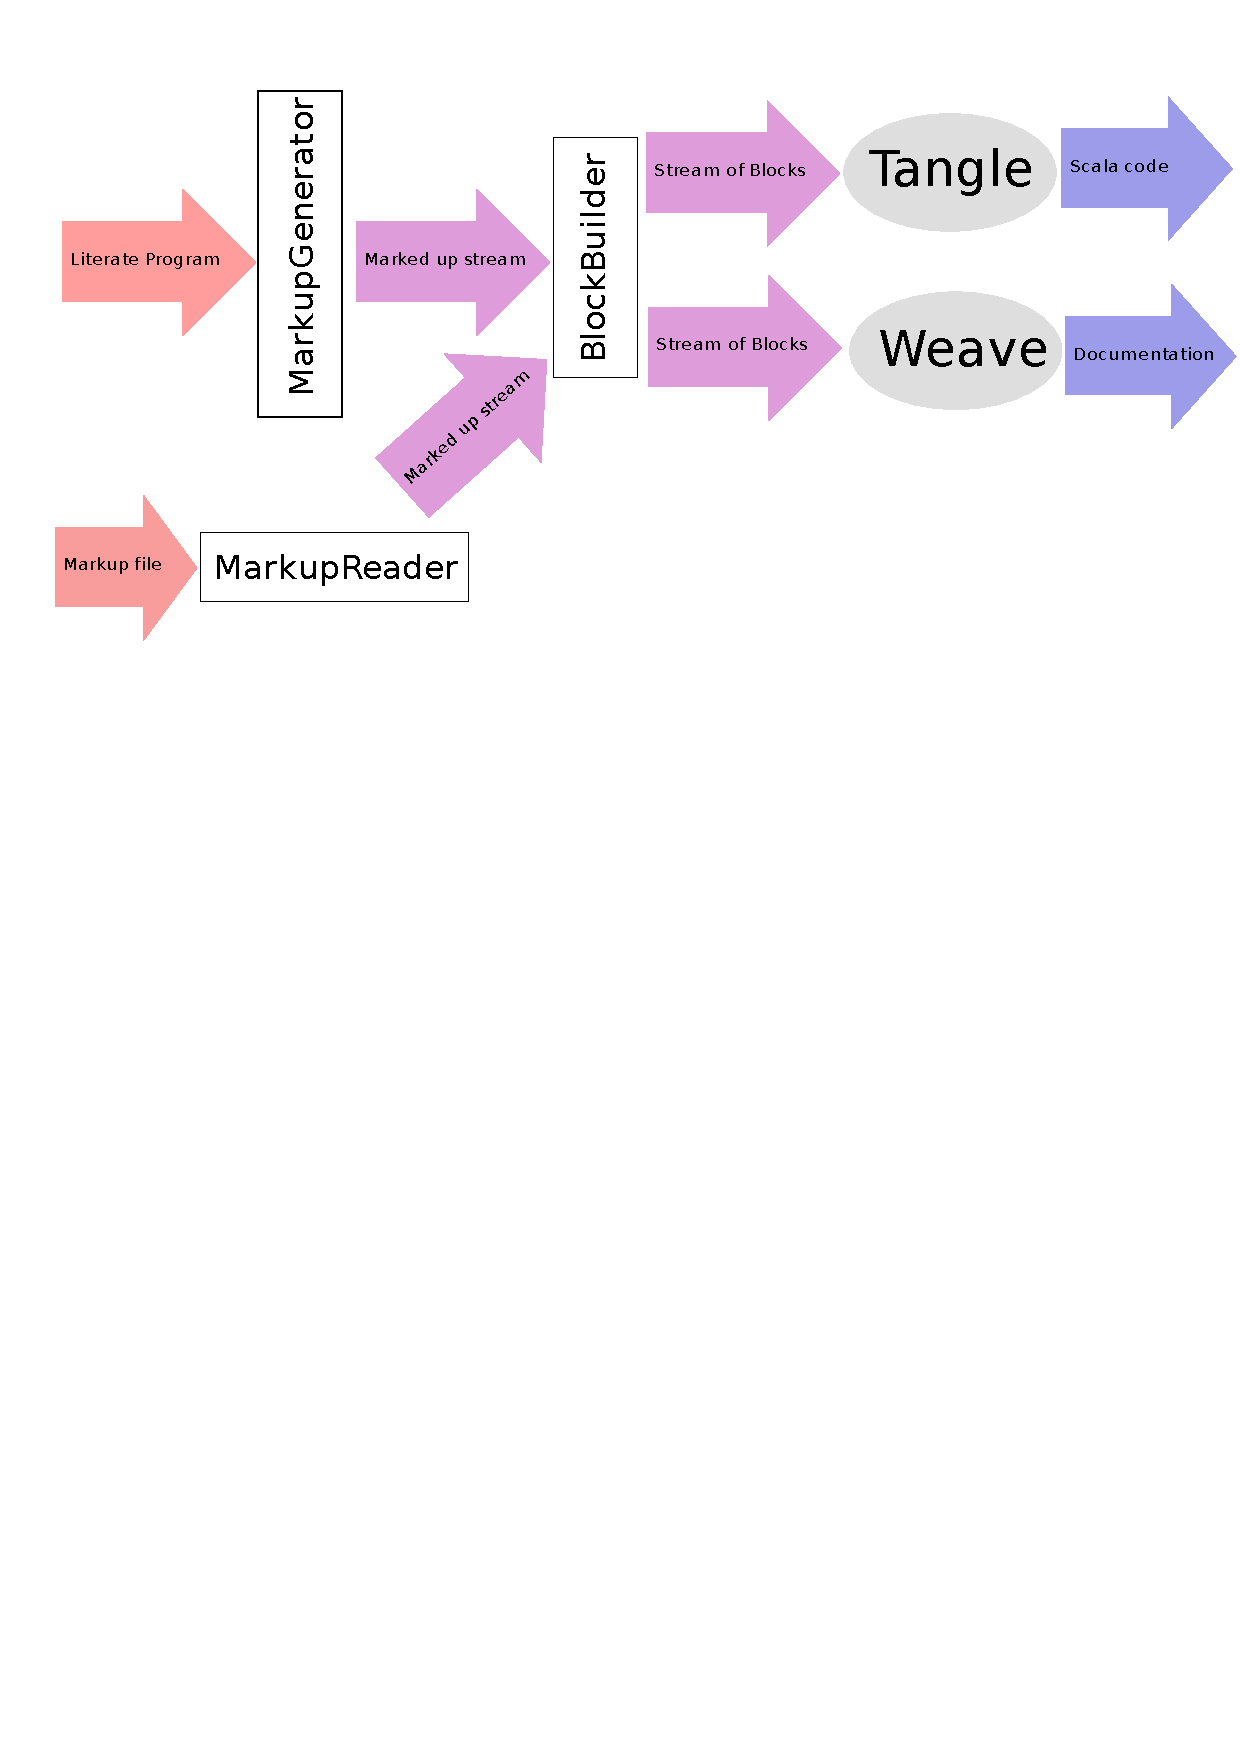
\includegraphics[width=16cm,viewport=0 550 800 800]{images/overview}

\subsection{Outline}
The Noweb markup that we will use is very light and only consists of
very few different cases, however, they all interact, so the conversion
part is still quite difficult. A noweb file will contain:

\begin{itemize}
\item source chunks (whose beginning is indicated by an @ sign)
\item quoted text (indicated by \texttt{[[} and \texttt{]]})
\item code chunks between \texttt{$\langle$$\langle$} and \texttt{$\rangle$$\rangle$=}
\item use directives (also between \texttt{$\langle$$\langle$} and \texttt{$\rangle$$\rangle$}, but without an =
afterwards
\end{itemize}

More details of the format can be found in the file \texttt{markup.nw} in the
noweb distribution\footnote{Noweb home page: http://www.eecs.harvard.edu/nr/noweb/}

This will then be converted in the intermediary format. To get a rough feeling for
the intermediary format, we will first treat this format and write the conversion
classes to this intermediary format afterwards:

$\left<\mbox{\emph{*}}\right>\equiv$
\begin{program}{\vem package}~scalit.markup
\\[0.5em]$<$line~types$>$
\\[0.5em]$<$read~in~the~intermediary~format$>$
\\[0.5em]$<$markup~reader$>$
\\[0.5em]$<$conversion~from~noweb~to~markup$>$
\\[0.5em]$<$markup~generator$>$
\\[0.5em]\end{program}
\subsection{The line types of the intermediary format}
There are about a dozen different line types. Let us first define these
line types and then consider how to read in a file in this format.

$\left<\mbox{\emph{line types}}\right>\equiv$
\begin{program}{\vem abstract}~{\vem class}~Line
\\[0.5em]\end{program}
Now for the subclasses

\begin{description}
\item[A line of text] Might occur inside documentation chunks but also
inside code chunks.

$\left<\mbox{\emph{line types}}\right>+\equiv$
\begin{program}{\vem case}~{\vem class}~TextLine$($content\,{\rm :}~String$)$~{\vem extends}~Line~{\small\{}
\\~~~~{\vem override}~{\vem def}~toString~=~"@text~"~$+$~content
\\{\small\}}
\\[0.5em]\end{program}
\item[A new line] Because we will be splitting up one line in different lines
describing the structure of the file, we will have to indicate when a newline
character occured in the source file. This is done with the following class:

$\left<\mbox{\emph{line types}}\right>+\equiv$
\begin{program}{\vem case}~{\vem object}~NewLine~{\vem extends}~Line~{\small\{}
\\~~~~{\vem override}~{\vem def}~toString~=~"@nl"
\\{\small\}}
\\[0.5em]\end{program}
\item[Quotes] Section of the text will be quoted and will appear verbatim
in the documentation. They are situated betwen beginning and end quote tokens:

$\left<\mbox{\emph{line types}}\right>+\equiv$
\begin{program}{\vem case}~{\vem object}~Quote~{\vem extends}~Line~{\small\{}
\\~~~~{\vem override}~{\vem def}~toString~=~"@quote"
\\{\small\}}
\\{\vem case}~{\vem object}~EndQuote~{\vem extends}~Line~{\small\{}
\\~~~~{\vem override}~{\vem def}~toString~=~"@endquote"
\\{\small\}}
\\[0.5em]\end{program}
\item[Code chunks] Like quotes, we will designate code chunks by their
beginning and end. Another important information will be the \emph{number} of
this chunk: Code and documentation chunks are numbered consecutively.

$\left<\mbox{\emph{line types}}\right>+\equiv$
\begin{program}{\vem case}~{\vem class}~Code$($number\,{\rm :}~Int$)$~{\vem extends}~Line~{\small\{}
\\~~~~{\vem override}~{\vem def}~toString~=~"@begin~code~"~$+$~number
\\{\small\}}
\\{\vem case}~{\vem class}~EndCode$($number\,{\rm :}~Int$)$~{\vem extends}~Line~{\small\{}
\\~~~~{\vem override}~{\vem def}~toString~=~"@end~code~"~$+$~number
\\{\small\}}
\\[0.5em]\end{program}
As already mentioned, code chunks will be given names so that they
can be used as part of other code chunks. This information will be the
first line inside a code section:

$\left<\mbox{\emph{line types}}\right>+\equiv$
\begin{program}{\vem case}~{\vem class}~Definition$($chunkname\,{\rm :}~String$)$~{\vem extends}~Line~{\small\{}
\\~~~~{\vem override}~{\vem def}~toString~=~"@defn~"~$+$~chunkname
\\{\small\}}
\\[0.5em]\end{program}
Now that we have a line indicating which code chunk is defined, we can
also envisage to use it in other code chunks:

$\left<\mbox{\emph{line types}}\right>+\equiv$
\begin{program}{\vem case}~{\vem class}~Use$($chunkname\,{\rm :}~String$)$~{\vem extends}~Line~{\small\{}
\\~~~~{\vem override}~{\vem def}~toString~=~"@use~"~$+$~chunkname
\\{\small\}}
\\[0.5em]\end{program}
\item[Documentation] Like code chunks, documentation chunks will be given
a number. Otherwise, they behave the same:

$\left<\mbox{\emph{line types}}\right>+\equiv$
\begin{program}{\vem case}~{\vem class}~Doc$($number\,{\rm :}~Int$)$~{\vem extends}~Line~{\small\{}
\\~~~~{\vem override}~{\vem def}~toString~=~"@begin~docs~"~$+$~number
\\{\small\}}
\\{\vem case}~{\vem class}~EndDoc$($number\,{\rm :}~Int$)$~{\vem extends}~Line~{\small\{}
\\~~~~{\vem override}~{\vem def}~toString~=~"@end~docs~"~$+$~number
\\{\small\}}
\\[0.5em]\end{program}
\item[Special indicators] We will have two special indicators: One telling us
which file we are reading and one to indicate the end of our input.

$\left<\mbox{\emph{line types}}\right>+\equiv$
\begin{program}{\vem case}~{\vem class}~File$($filename\,{\rm :}~String$)$~{\vem extends}~Line~{\small\{}
\\~~~~{\vem override}~{\vem def}~toString~=~"@file~"~$+$~filename
\\{\small\}}
\\{\vem case}~{\vem object}~LastLine~{\vem extends}~Line
\\[0.5em]\end{program}
\end{description}

To test whether the intermediary format was completely described, we
will build a small parser for it in the next section.

\subsection{Reading in the intermediary format}

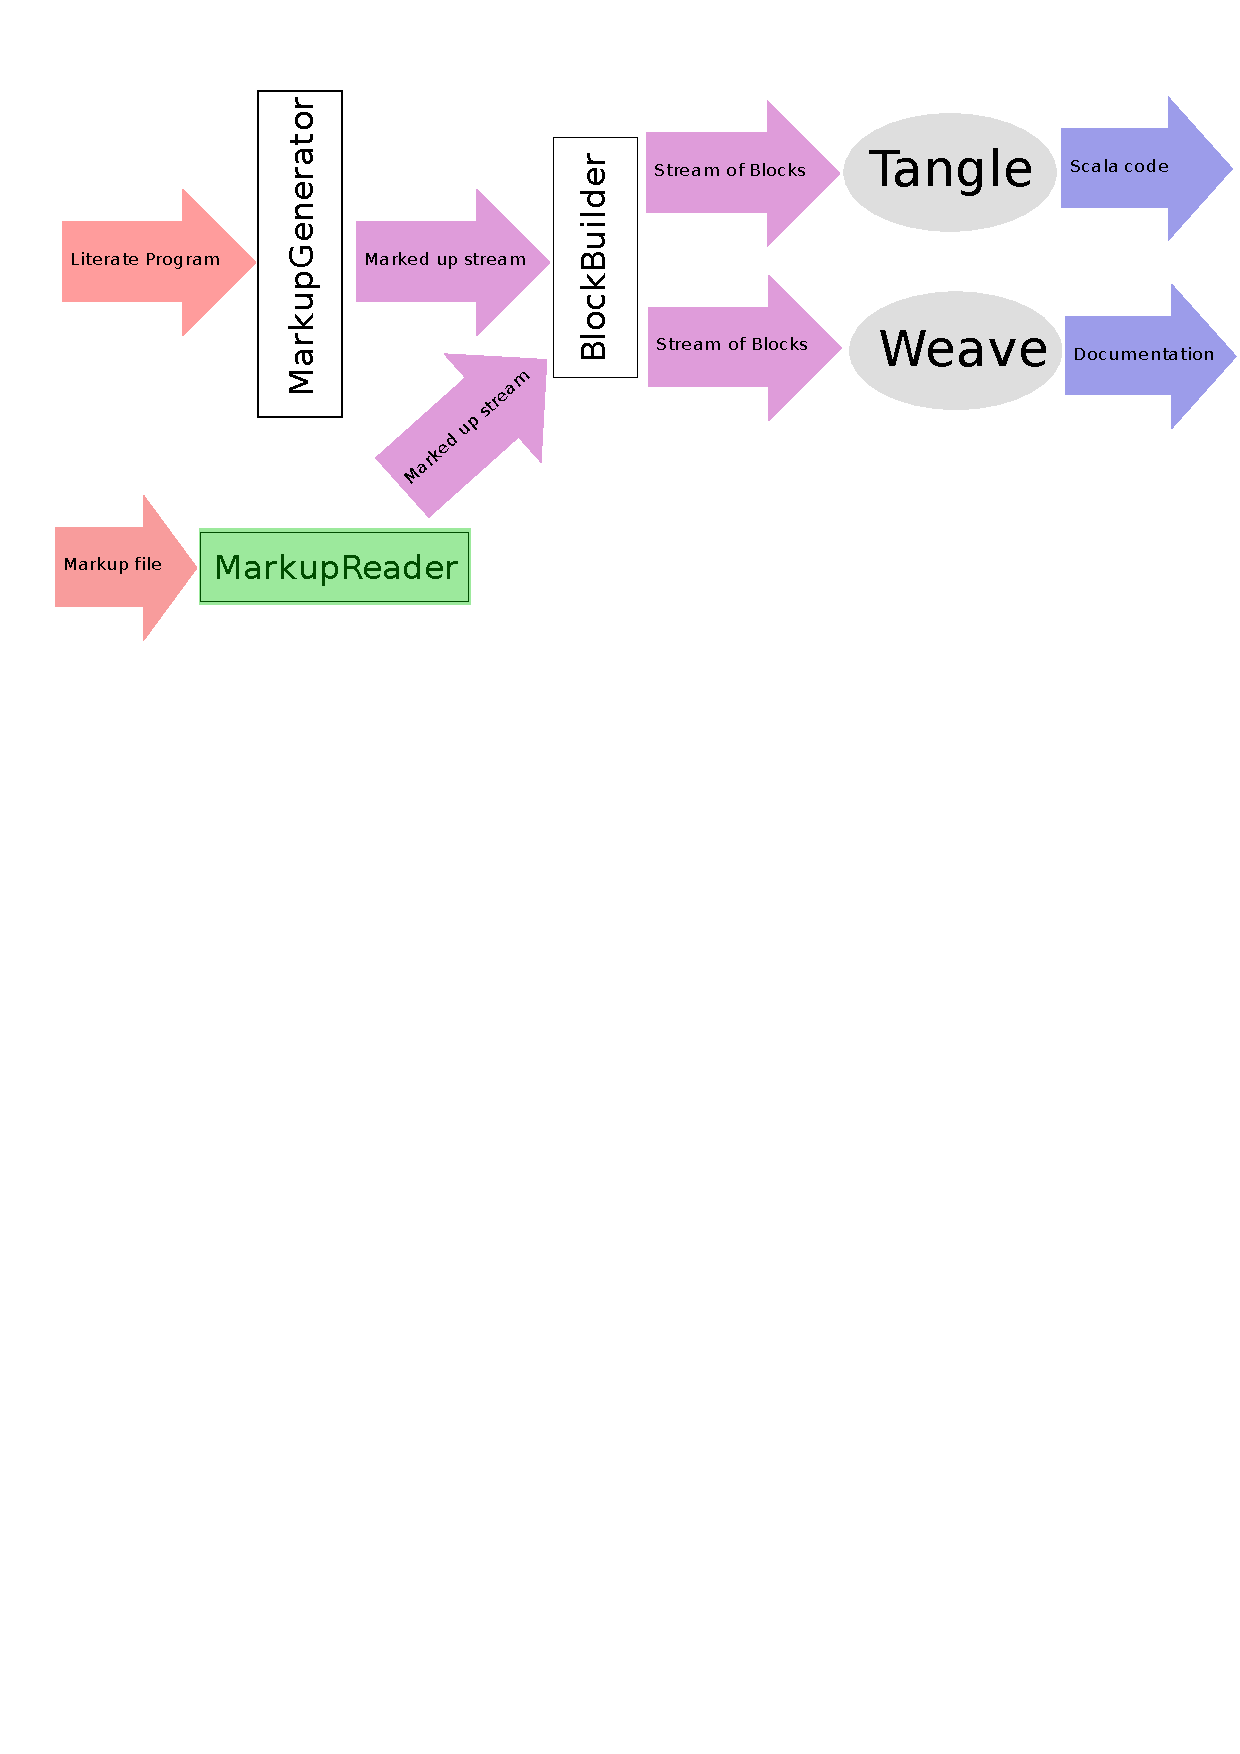
\includegraphics[viewport=0 500 264 800,clip,height=7cm]{images/markupReader.pdf}

A parser for the intermediary format will be much simpler than the one
we will have to build for the noweb source format: It suffices to parse
the beginning of a line to get the function. This simple parser will
consist of two methods, one that gets the next token and one that
represents all the tokens of a file as a stream.

$\left<\mbox{\emph{read in the intermediary format}}\right>\equiv$
\begin{program}{\vem import}~scala.util.parsing.input.StreamReader
\\{\vem class}~MarkupParser$($in\,{\rm :}~StreamReader$)$~{\small\{}
\\~~~~$<$get~next~token~of~markup~file$>$
\\~~~~$<$token~stream~of~markup~file$>$
\\{\small\}}
\\[0.5em]\end{program}
Note that the MarkupParser takes a stream reader representation of
the input file as constructor argument. With a StreamReader, we have
the possibility to record our position in the file while reading.

Let us first look at the stream representation: We know we have read the
last token when we see \texttt{LastLine}

$\left<\mbox{\emph{token stream of markup file}}\right>\equiv$
\begin{program}{\vem def}~lines\,{\rm :}~Stream$[$Line$]$~=~{\small\{}
\\~~~~{\vem def}~lines0$($input\,{\rm :}~StreamReader$)${\rm :}~Stream$[$Line$]$~=
\\~~~~nextToken$($input$)$~{\vem match}~{\small\{}
\\~~~~~~~~{\vem case}~$($LastLine,rest$)$~$\Rightarrow$~Stream.empty
\\~~~~~~~~{\vem case}~$($line,rest$)$~$\Rightarrow$~Stream.cons$($line,~lines0$($rest$)$$)$
\\~~~~{\small\}}
\\~~~~lines0$($in$)$
\\{\small\}}
\\[0.5em]\end{program}
After we have read the token, we will have advanced in the stream, therefore
we will read in the next token from the returned position.

This stream representation will be quite useful when we are processing
the input with tangle and weave. But let us move on to the method that
actually gives us the token:

$\left<\mbox{\emph{get next token of markup file}}\right>\equiv$
\begin{program}{\vem def}~nextToken$($input\,{\rm :}~StreamReader$)${\rm :}~$($Line,StreamReader$)$~=~{\small\{}
\\~~~~{\vem def}~readLine$($inreader\,{\rm :}~StreamReader,
\\~~~~~~~~~~~~~~~~~~~~~~acc\,{\rm :}~List$[$Char$]$$)${\rm :}~$($List$[$Char$]$,StreamReader$)$~=
\\~~~~~~~~{\vem if}$($~inreader.atEnd~$\,|$$\,|$~inreader.first~$==$~'$\backslash$n'~$)$
\\~~~~~~~~~~~~$($inreader.first~{\rm :}{\rm :}~acc.reverse,~inreader.rest~$)$
\\~~~~~~~~{\vem else}~readLine$($inreader.rest,~inreader.first~{\rm :}{\rm :}~acc~$)$
\\[0.5em]\end{program}
This little function reads in the whole line and returns the position
afterwards.

$\left<\mbox{\emph{get next token of markup file}}\right>+\equiv$
\begin{program}~~~~in.first~{\vem match}~{\small\{}
\\~~~~~~~~{\vem case}~'@'~$\Rightarrow$~{\small\{}
\\~~~~~~~~~~~~{\vem val}~$($line,rest$)$~=~readLine$($input.rest,Nil$)$
\\~~~~~~~~~~~~{\vem val}~directive~=~$<${\vem match}~on~the~directive~to~produce~the~line$>$
\\~~~~~~~~~~~~$($directive,rest$)$
\\~~~~~~~~{\small\}}
\\~~~~~~~~{\vem case}~\_~$\Rightarrow$
\\~~~~~~~~~~~~System.err.println$($"Found~a~line~not~beginning"~$+$
\\~~~~~~~~~~~~~~~~~~~~~~~~~~~~~~~~~~"~{\vem with}~@,~but~{\vem with}~"~$+$
\\~~~~~~~~~~~~~~~~~~~~~~~~~~~~~~~~~~input.first$)$
\\~~~~~~~~~~~~exit$($1$)$
\\~~~~{\small\}}
\\{\small\}}
\\[0.5em]\end{program}
When having read a line, we take the directive which is everything before
the first space character. So we split along the spaces. However, strangely
enough the readLine function (and therefore StreamReader) seems to insert
a strange character at the beginning (this might as well be a bug), so we will
have to continue after that.

$\left<\mbox{\emph{match on the directive to produce the line}}\right>\equiv$
\begin{program}$($line.tail~mkString~""~split~'~'$)$.toList~{\vem match}~{\small\{}
\\~~~~{\vem case}~"file"~{\rm :}{\rm :}~sth~$\Rightarrow$~File$($sth~mkString~"~"$)$
\\[0.5em]\end{program}
The file line has one more argument: The filename. We thus simply reconstruct
it from the argument list.

After the file token, we will usually find a beginning of either a code or
a documentation chunk. The only argument this takes is the chunk number.

$\left<\mbox{\emph{match on the directive to produce the line}}\right>+\equiv$
\begin{program}~~~~{\vem case}~"begin"~{\rm :}{\rm :}~"docs"~{\rm :}{\rm :}~number~{\rm :}{\rm :}~Nil~$\Rightarrow$
\\~~~~~~~~Doc$($Integer.parseInt$($number$)$$)$
\\~~~~{\vem case}~"begin"~{\rm :}{\rm :}~"code"~{\rm :}{\rm :}~number~{\rm :}{\rm :}~Nil~$\Rightarrow$
\\~~~~~~~~Code$($Integer.parseInt$($number$)$$)$
\\[0.5em]\end{program}
The beginning directive will be matched by the same end directive:

$\left<\mbox{\emph{match on the directive to produce the line}}\right>+\equiv$
\begin{program}~~~~{\vem case}~"end"~{\rm :}{\rm :}~"docs"~{\rm :}{\rm :}~number~{\rm :}{\rm :}~Nil~$\Rightarrow$
\\~~~~~~~~EndDoc$($Integer.parseInt$($number$)$$)$
\\~~~~{\vem case}~"end"~{\rm :}{\rm :}~"code"~{\rm :}{\rm :}~number~{\rm :}{\rm :}~Nil~$\Rightarrow$
\\~~~~~~~~EndCode$($Integer.parseInt$($number$)$$)$
\\[0.5em]\end{program}
Inside this documentation block, we may find text parts and newlines, primarily,
which we will match in the same way. A quick note on the text: This is whitespace
sensitive (the line will quite likely end in whitespace), therefore we do pass
it the line and not the split.

$\left<\mbox{\emph{match on the directive to produce the line}}\right>+\equiv$
\begin{program}~~~~{\vem case}~"text"~{\rm :}{\rm :}~content~$\Rightarrow$
\\~~~~~~~~TextLine$($line~drop~6~mkString~""$)$
\\~~~~{\vem case}~"nl"~{\rm :}{\rm :}~Nil~$\Rightarrow$
\\~~~~~~~~NewLine
\\[0.5em]\end{program}
Inside code chunks, we will also find indications on how the chunk is called:

$\left<\mbox{\emph{match on the directive to produce the line}}\right>+\equiv$
\begin{program}~~~~{\vem case}~"defn"~{\rm :}{\rm :}~chunkname~$\Rightarrow$~Definition$($chunkname~mkString~"~"$)$
\\[0.5em]\end{program}
Use directives work the same way:

$\left<\mbox{\emph{match on the directive to produce the line}}\right>+\equiv$
\begin{program}~~~~{\vem case}~"use"~{\rm :}{\rm :}~chunkname~$\Rightarrow$~Use$($chunkname~mkString~"~"$)$
\\[0.5em]\end{program}
Quote and EndQuote do not take any parameters:

$\left<\mbox{\emph{match on the directive to produce the line}}\right>+\equiv$
\begin{program}~~~~{\vem case}~"quote"~{\rm :}{\rm :}~Nil~$\Rightarrow$~Quote
\\~~~~{\vem case}~"endquote"~{\rm :}{\rm :}~Nil~$\Rightarrow$~EndQuote
\\[0.5em]\end{program}
If we see an empty string, then we will have arrived at the last line.
Otherwise, do mark the token as unrecognized.

$\left<\mbox{\emph{match on the directive to produce the line}}\right>+\equiv$
\begin{program}~~~~{\vem case}~""~{\rm :}{\rm :}~Nil~$\Rightarrow$~LastLine
\\~~~~{\vem case}~unrecognized~$\Rightarrow$~{\small\{}
\\~~~~~~~~System.err.println$($"Unrecognized~directive\,{\rm :}~"~$+$
\\~~~~~~~~~~~~~~~~~~~~~~~~~~~~~~~~~~unrecognized.head.size$)$
\\~~~~~~~~println$($input.pos$)$
\\~~~~~~~~LastLine
\\~~~~{\small\}}
\\{\small\}}
\\[0.5em]\end{program}
\subsubsection{Testing the markup format}
Like the Markup generator, we also want to test the markup reader.
We will output what we have read in to compare it to the original
file: If we get the same result, then we are fine.

$\left<\mbox{\emph{markup reader}}\right>\equiv$
\begin{program}{\vem object}~MarkupReader~{\small\{}
\\~~~~{\vem import}~java.io.{\small\{}FileReader,BufferedReader,Reader{\small\}}
\\~~~~{\vem import}~java.io.InputStreamReader
\\[0.5em]~~~~{\vem def}~usage~=
\\~~~~~~~~println$($"Usage\,{\rm :}~scala~markup.MarkupReader~$[$infile$]$"$)$
\\[0.5em]~~~~{\vem def}~main$($args\,{\rm :}~Array$[$String$]$$)$~=~{\small\{}
\\~~~~~~~~{\vem val}~input\,{\rm :}~Reader~=~args.length~{\vem match}~{\small\{}
\\~~~~~~~~~~~~{\vem case}~0~$\Rightarrow$~{\vem new}~InputStreamReader$($System.in$)$
\\~~~~~~~~~~~~{\vem case}~1~$\Rightarrow$~{\vem new}~BufferedReader$(${\vem new}~FileReader$($args$($0$)$$)$$)$
\\~~~~~~~~~~~~{\vem case}~\_~$\Rightarrow$~usage;~exit
\\~~~~~~~~{\small\}}
\\~~~~~~~~{\vem val}~markupReader~=~{\vem new}~MarkupParser$($StreamReader$($input$)$$)$
\\~~~~~~~~markupReader.lines~foreach~{\small\{}
\\~~~~~~~~~~~~line~$\Rightarrow$~println$($line$)$
\\~~~~~~~~{\small\}}
\\~~~~{\small\}}
\\{\small\}}
\\[0.5em]\end{program}
Very basic: We either get a file name as argument or we treat standard input. For
this test, we will just print the lines stream.


\subsection{Converting from the input}

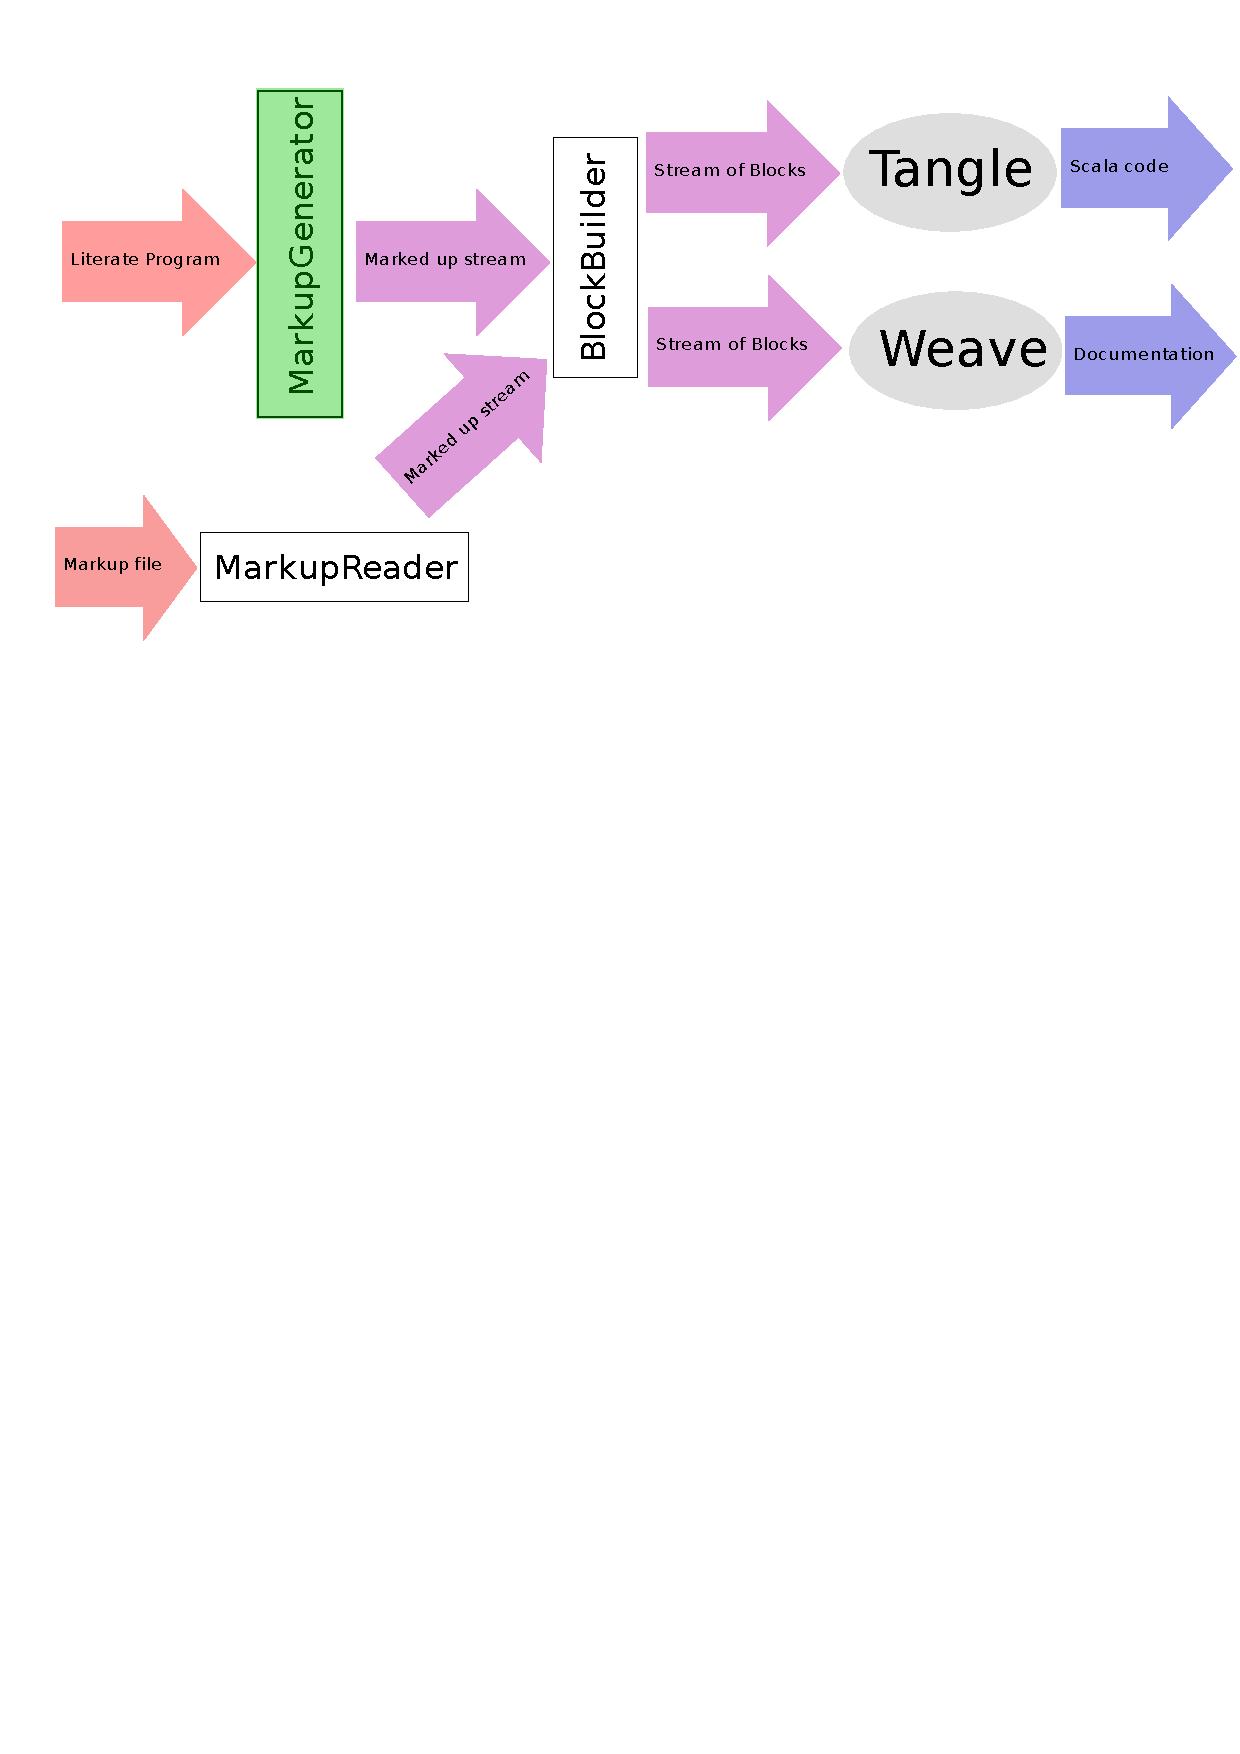
\includegraphics[viewport=0 500 264 800,clip,height=7cm]{images/markupGenerator.pdf}
Now that we know enough about the intermediary format, we are ready to
treat the conversion. The final product will be a stream of markup lines
(like we used them above). The first token will be the filename:

$\left<\mbox{\emph{conversion from noweb to markup}}\right>\equiv$
\begin{program}{\vem class}~MarkupGenerator$($in\,{\rm :}~StreamReader,~filename\,{\rm :}~String$)$~{\small\{}
\\~~~~{\vem def}~lines\,{\rm :}~Stream$[$Line$]$~=
\\~~~~~~~~Stream.cons$($File$($filename$)$,
\\~~~~~~~~Stream.cons$($Doc$($0$)$,documentation$($in,0$)$$)$$)$
\\~~~~$<$in~documentation~mode$>$
\\~~~~$<$in~quote~mode$>$
\\~~~~$<$in~code~mode$>$
\\[0.5em]~~~~$<$read~chunk~name$>$
\\~~~~$<$read~use~name$>$
\\[0.5em]~~~~$<$tab~handling$>$
\\{\small\}}
\\[0.5em]\end{program}
The second token is also already given: The start of the first documentation
block. A noweb file will always start with a block like this. The next section
defines how the documentation mode works.

\subsubsection{The documentation mode}
The documentation mode will accumulate TextLines and NewLines as long as we
do not see a combination that would terminate this documentation chunk:

\begin{itemize}
\item Another documentation chunk (at sign on a new line)
\item A quoted section
\item Beginning of a code block
\end{itemize}

To memorize the line content, we will use an accumulator.

$\left<\mbox{\emph{in documentation mode}}\right>\equiv$
\begin{program}~~~~~~{\vem def}~documentation$($inp\,{\rm :}~StreamReader,
\\~~~~~~~~~~~~~~~~~~~~~~~~~~~~~~~~docnumber\,{\rm :}~Int$)${\rm :}~Stream$[$Line$]$~=~{\small\{}
\\~~~~~~~~~~{\vem def}~docAcc$($input\,{\rm :}~StreamReader,
\\~~~~~~~~~~~~~~~~~~~~~~~~~~acc\,{\rm :}~List$[$Char$]$$)${\rm :}~Stream$[$Line$]$~=
\\~~~~~~~~~~~~~~$<$accumulate~in~doc~mode$>$
\\[0.5em]~~~~~~~~~~docAcc$($inp,Nil$)$
\\~~~~~~{\small\}}
\\[0.5em]\end{program}
Now let us look at how to produce some lines:

$\left<\mbox{\emph{accumulate in doc mode}}\right>\equiv$
\begin{program}~~input.first~{\vem match}~{\small\{}
\\~~~~~~{\vem case}~'$[$'~$\Rightarrow$~input.rest.first~{\vem match}~{\small\{}
\\~~~~~~~~~~{\vem case}~'$[$'~$\Rightarrow$
\\~~~~~~~~~~~~~~{\vem val}~$($content,continue$)$~=~quote$($input.rest.rest$)$
\\~~~~~~~~~~~~~~acc~{\vem match}~{\small\{}
\\~~~~~~~~~~~~~~~~~~{\vem case}~Nil~$\Rightarrow$
\\~~~~~~~~~~~~~~~~~~~~~~Stream.concat$($
\\~~~~~~~~~~~~~~~~~~~~~~~~~~Stream.cons$($Quote,content$)$,
\\~~~~~~~~~~~~~~~~~~~~~~~~~~Stream.cons$($EndQuote,
\\~~~~~~~~~~~~~~~~~~~~~~~~~~~~~~~~~~~~~~~~~~~~~~docAcc$($continue,Nil$)$$)$$)$
\\~~~~~~~~~~~~~~~~~~{\vem case}~\_~~~$\Rightarrow$
\\~~~~~~~~~~~~~~~~~~~~~~Stream.concat$($
\\~~~~~~~~~~~~~~~~~~~~~~~~~~Stream.cons$($TextLine$($acc.reverse~mkString~""$)$,
\\~~~~~~~~~~~~~~~~~~~~~~~~~~Stream.cons$($Quote,
\\~~~~~~~~~~~~~~~~~~~~~~~~~~~~~~~~~~~~~~~~~~~~content$)$$)$,
\\~~~~~~~~~~~~~~~~~~~~~~~~~~Stream.cons$($EndQuote,
\\~~~~~~~~~~~~~~~~~~~~~~~~~~~~~~~~~~~~~~~~~~~~docAcc$($continue,Nil$)$$)$$)$
\\~~~~~~~~~~~~~~{\small\}}
\\~~~~{\vem case}~\_~$\Rightarrow$~docAcc$($input.rest,~input.first~{\rm :}{\rm :}~acc$)$
\\{\small\}}
\\[0.5em]\end{program}
If we encounter the beginning of a quoted section, then we will call
the quote mode just to continue parsing afterwards. If we encounter the
at sign at the beginning of a line, we will start a new documentation chunk:

$\left<\mbox{\emph{accumulate in doc mode}}\right>+\equiv$
\begin{program}~~{\vem case}~'@'~$\Rightarrow$~acc~{\vem match}~{\small\{}
\\~~~~~~{\vem case}~Nil~$\Rightarrow$
\\~~~~~~~~~~{\vem if}$($~input.rest.first~$==$~'$\backslash$n'~$\,|$$\,|$
\\~~~~~~~~~~~~~~~~~~~~~~~~~~~~~~~~input.rest.first~$==$~'~'~$)$
\\~~~~~~~~~~~~~~Stream.cons$($EndDoc$($docnumber$)$,
\\~~~~~~~~~~~~~~Stream.cons$($Doc$($docnumber~$+$~1$)$,
\\~~~~~~~~~~~~~~~~~~~~~~~~~~~~~~~~documentation$($input.rest.rest,docnumber~$+$~1$)$$)$$)$
\\~~~~~~~~~~{\vem else}
\\~~~~~~~~~~~~~~docAcc$($input.rest,~List$($'@'$)$$)$
\\~~~~~~{\vem case}~\_~$\Rightarrow$~docAcc$($input.rest,~'@'~{\rm :}{\rm :}~acc$)$
\\~~{\small\}}
\\[0.5em]\end{program}
A documentation section can also be terminated by the beginning of a
code chunk. This chunk will be between \texttt{$\langle$$\langle$} and \texttt{$\rangle$$\rangle$=}. If a code
chunk seems to be opened but a newline follows before it was closed,
we have to report this error:

$\left<\mbox{\emph{accumulate in doc mode}}\right>+\equiv$
\begin{program}~~{\vem case}~'$<$'~$\Rightarrow$~input.rest.first~{\vem match}~{\small\{}
\\~~~~~~{\vem case}~'$<$'~$\Rightarrow$~acc~{\vem match}~{\small\{}
\\~~~~~~~~~~{\vem case}~x~{\rm :}{\rm :}~xs~$\Rightarrow$
\\~~~~~~~~~~~~~~~~~~~~~~~~~~~~~~error$($"Unescaped~$<\!$$<$~in~doc~mode"$)$
\\~~~~~~~~~~{\vem case}~Nil~$\Rightarrow$
\\~~~~~~~~~~~~~~~~~~{\vem val}~$($chunkName,continue$)$~=~chunkDef$($input.rest.rest$)$
\\~~~~~~~~~~~~~~~~~~Stream.cons$($EndDoc$($docnumber$)$,
\\~~~~~~~~~~~~~~~~~~Stream.cons$($Code$($docnumber~$+$~1$)$,
\\~~~~~~~~~~~~~~~~~~~~~~code$($continue,chunkName,docnumber$+$1$)$$)$$)$
\\~~~~~~{\small\}}
\\~~~~~~{\vem case}~\_~$\Rightarrow$~docAcc$($input.rest,~'$<$'~{\rm :}{\rm :}~acc$)$
\\~~{\small\}}
\\[0.5em]\end{program}
If we were able to read a chunk name, we will open a new code section
with this information.

$\left<\mbox{\emph{accumulate in doc mode}}\right>+\equiv$
\begin{program}~~{\vem case}~c~$\Rightarrow$
\\~~~~~~{\vem if}$($~c~$==$~'$\backslash$n'~$)$~{\small\{}
\\~~~~~~~~~~Stream.cons$($TextLine$($acc.reverse~mkString~""$)$,
\\~~~~~~~~~~Stream.cons$($NewLine,docAcc$($input.rest,Nil$)$$)$$)$
\\~~~~~~{\small\}}~{\vem else}~{\small\{}
\\~~~~~~~~~~{\vem if}$($~!input.atEnd~$)$~docAcc$($input.rest,input.first~{\rm :}{\rm :}~acc$)$
\\~~~~~~~~~~{\vem else}~acc~{\vem match}~{\small\{}
\\~~~~~~~~~~~~~~{\vem case}~Nil~$\Rightarrow$~Stream.cons$($EndDoc$($docnumber$)$,
\\~~~~~~~~~~~~~~~~~~~~~~~~~~~~~~~~~~~~~~~~~~~~~~~~~~~~~~~~~~Stream.empty$)$
\\~~~~~~~~~~~~~~{\vem case}~\_~$\Rightarrow$
\\~~~~~~~~~~~~~~~~~~Stream.cons$($TextLine$($acc.reverse~mkString~""$)$,
\\~~~~~~~~~~~~~~~~~~Stream.cons$($NewLine,
\\~~~~~~~~~~~~~~~~~~Stream.cons$($EndDoc$($docnumber$)$,Stream.empty$)$$)$$)$
\\~~~~~~~~~~{\small\}}
\\~~~~~~{\small\}}
\\~~{\small\}}
\\[0.5em]\end{program}
As a general rule, all markup files will have a newline at the end. If
no newline is there, then we will add one.

\subsubsection{The quote mode}
In quote mode, we will ignore all normal control characters up until the
point where we encounter the close quote \texttt{]]}. Note, however, that additional
\texttt{]}s have to be taken into account: The quote is only closed with the
last \texttt{]} in a row.

$\left<\mbox{\emph{in quote mode}}\right>\equiv$
\begin{program}{\vem def}~quote$($inp\,{\rm :}~StreamReader$)${\rm :}~$($Stream$[$Line$]$,~StreamReader$)$~=~{\small\{}
\\~~~~{\vem def}~quoteAcc$($input\,{\rm :}~StreamReader,~acc\,{\rm :}~List$[$Char$]$$)${\rm :}
\\~~~~~~~~~~$($Stream$[$Line$]$,~StreamReader$)$~=
\\~~input.first~{\vem match}~{\small\{}
\\~~~~~~{\vem case}~'$]$'~$\Rightarrow$~input.rest.first~{\vem match}~{\small\{}
\\~~~~~~~~~~{\vem case}~'$]$'~$\Rightarrow$~input.rest.rest.first~{\vem match}~{\small\{}
\\~~~~~~~~~~~~~~{\vem case}~'$]$'~$\Rightarrow$~quoteAcc$($input.rest,'$]$'~{\rm :}{\rm :}~acc$)$
\\~~~~~~~~~~~~~~{\vem case}~\_~$\Rightarrow$~acc~{\vem match}~{\small\{}
\\~~~~~~~~~~~~~~~~~~{\vem case}~Nil~$\Rightarrow$~$($Stream.empty,input.rest.rest$)$
\\~~~~~~~~~~~~~~~~~~{\vem case}~\_~$\Rightarrow$~$($Stream.cons$($TextLine$($acc.reverse~mkString~""$)$,
\\~~~~~~~~~~~~~~~~~~~~~~~~~~~~~~~~~~~~~~~~~~~~~~~~~~~~~~~~~~~~~~~~Stream.empty$)$,
\\~~~~~~~~~~~~~~~~~~~~~~~~~~~~~~~~~~~~~~~~input.rest.rest$)$
\\~~~~~~~~~~~~~~{\small\}}
\\~~~~~~~~~~{\small\}}
\\~~~~~~~~~~{\vem case}~\_~$\Rightarrow$~quoteAcc$($input.rest,'$]$'~{\rm :}{\rm :}~acc$)$
\\~~~~~~{\small\}}
\\~~~~~~{\vem case}~'$\backslash$n'~$\Rightarrow$~acc~{\vem match}~{\small\{}
\\~~~~~~~~~~{\vem case}~Nil~$\Rightarrow$~{\vem val}~$($more,contreader$)$~=~quoteAcc$($input.rest,Nil$)$
\\~~~~~~~~~~~~~~~~~~~~~~~~~~~~~~~~~~$($Stream.cons$($NewLine,more$)$,contreader$)$
\\~~~~~~~~~~{\vem case}~\_~$\Rightarrow$~{\vem val}~$($more,contreader$)$~=~quoteAcc$($input.rest,Nil$)$
\\~~~~~~~~~~~~~~~~~~~~~~~~~~~~~~$($Stream.cons$($TextLine$($acc.reverse~mkString~""$)$,
\\~~~~~~~~~~~~~~~~~~~~~~~~~~~~~~Stream.cons$($NewLine,~more$)$$)$,contreader$)$
\\~~~~~~{\small\}}
\\~~~~~~{\vem case}~c~$\Rightarrow$~quoteAcc$($input.rest,~c~{\rm :}{\rm :}~acc$)$
\\~~{\small\}}
\\~~~~~~~~~~~~~~quoteAcc$($inp,Nil$)$
\\{\small\}}
\\[0.5em]\end{program}
\subsubsection{The code mode}
Code chunks are a bit different from documentation chunks in the fact that
they are named. The following method reads the name of a documentation chunk
and returns it:

$\left<\mbox{\emph{read chunk name}}\right>\equiv$
\begin{program}{\vem def}~chunkDef$($inp\,{\rm :}~StreamReader$)${\rm :}~$($String,~StreamReader$)$~=~{\small\{}
\\~~~~{\vem def}~chunkAcc$($input\,{\rm :}~StreamReader,~acc\,{\rm :}~List$[$Char$]$$)${\rm :}
\\~~~~$($String,~StreamReader$)$~=
\\~~~~input.first~{\vem match}~{\small\{}
\\~~~~~~~~{\vem case}~'$>$'~$\Rightarrow$~input.rest.first~{\vem match}~{\small\{}
\\~~~~~~~~~~~~{\vem case}~'$>$'~$\Rightarrow$~input.rest.rest.first~{\vem match}~{\small\{}
\\~~~~~~~~~~~~{\vem case}~'='~$\Rightarrow$~$($$($acc.reverse~mkString~""$)$,input.rest.rest.rest$)$
\\~~~~~~~~~~~~{\vem case}~\_~$\Rightarrow$~System.err.println$($"Unescaped"$)$;~exit
\\~~~~~~~~{\small\}}
\\~~~~~~~~{\vem case}~\_~$\Rightarrow$~chunkAcc$($input.rest,~'$>$'~{\rm :}{\rm :}~acc$)$
\\~~~~{\small\}}
\\~~~~{\vem case}~c~$\Rightarrow$~chunkAcc$($input.rest,~c~{\rm :}{\rm :}~acc$)$
\\~~~~{\small\}}
\\[0.5em]~~~~chunkAcc$($inp,~Nil$)$
\\{\small\}}
\\[0.5em]\end{program}
Now that we know how we can read in the chunk name, let us look on how to
read code sections:

$\left<\mbox{\emph{in code mode}}\right>\equiv$
\begin{program}{\vem def}~code$($inp\,{\rm :}~StreamReader,~chunkname\,{\rm :}~String,~codenumber\,{\rm :}~Int$)${\rm :}
\\~~~~Stream$[$Line$]$~=~{\small\{}
\\~~~~~~$<$detect~{\vem new}~code~chunk$>$
\\~~~~~~$<$detect~{\vem new}~use~directive$>$
\\~~~~{\vem def}~codeAcc$($input\,{\rm :}~StreamReader,~acc\,{\rm :}~List$[$Char$]$$)${\rm :}
\\~~~~~~~~Stream$[$Line$]$~=~input.first~{\vem match}~{\small\{}
\\~~~~~~~~~~~~{\vem case}~'$<$'~$\Rightarrow$~input.rest.first~{\vem match}~{\small\{}
\\~~~~~~~~~~~~~~~~{\vem case}~'$<$'~$\Rightarrow$
\\~~~~~~~~~~~~~~~~~~~~acc~{\vem match}~{\small\{}
\\~~~~~~~~~~~~~~~~~~~~~~~~{\vem case}~Nil~$\Rightarrow$
\\~~~~~~~~~~~~~~~~~~~~~~~~{\vem if}$($~isNewCodeChunk$($input.rest.rest$)$~$)$~{\small\{}
\\~~~~~~~~~~~~~~~~~~~~~~~~~~~~{\vem val}~$($chunkName,continue$)$~=
\\~~~~~~~~~~~~~~~~~~~~~~~~~~~~~~~~chunkDef$($input.rest.rest$)$
\\~~~~~~~~~~~~~~~~~~~~~~~~~~~~Stream.cons$($EndCode$($codenumber$)$,
\\~~~~~~~~~~~~~~~~~~~~~~~~~~~~Stream.cons$($Code$($codenumber~$+$~1$)$,
\\~~~~~~~~~~~~~~~~~~~~~~~~~~~~~~~~code$($continue,
\\~~~~~~~~~~~~~~~~~~~~~~~~~~~~~~~~chunkName,
\\~~~~~~~~~~~~~~~~~~~~~~~~~~~~~~~~codenumber~$+$~1$)$$)$$)$
\\~~~~~~~~~~~~~~~~~~~~~~~~{\small\}}~{\vem else}~{\vem if}$($~isNewUseDirective$($input.rest$)$~$)$~{\small\{}
\\~~~~~~~~~~~~~~~~~~~~~~~~~~~~{\vem val}~$($usename,cont$)$~=~use$($input.rest.rest$)$
\\~~~~~~~~~~~~~~~~~~~~~~~~~~~~Stream.cons$($Use$($usename$)$,
\\~~~~~~~~~~~~~~~~~~~~~~~~~~~~~~~~~~~~codeAcc$($cont,Nil$)$$)$
\\~~~~~~~~~~~~~~~~~~~~~~~~{\small\}}~{\vem else}~{\small\{}
\\~~~~~~~~~~~~~~~~~~~~~~~~~~~~codeAcc$($input.rest,'$<$'~{\rm :}{\rm :}~acc$)$
\\~~~~~~~~~~~~~~~~~~~~~~~~{\small\}}
\end{program}
If we are not at the beginning of a line (\texttt{acc} is not empty), then
we don't have to worry about new code chunks, just use directives:

$\left<\mbox{\emph{in code mode}}\right>+\equiv$
\begin{program}~~~~~~~~~~~~~~~~~~~~~~~~{\vem case}~\_~$\Rightarrow$
\\~~~~~~~~~~~~~~~~~~~~~~~~{\vem if}$($~isNewUseDirective$($input.rest$)$~$)$~{\small\{}
\\~~~~~~~~~~~~~~~~~~~~~~~~~~~~{\vem val}~$($usename,cont$)$~=~use$($input.rest.rest$)$
\\~~~~~~~~~~~~~~~~~~~~~~~~~~~~Stream.cons$($TextLine$($acc.reverse~mkString~""$)$,
\\~~~~~~~~~~~~~~~~~~~~~~~~~~~~Stream.cons$($Use$($usename$)$,
\\~~~~~~~~~~~~~~~~~~~~~~~~~~~~~~~~codeAcc$($cont,~Nil$)$$)$$)$
\\~~~~~~~~~~~~~~~~~~~~~~~~{\small\}}~{\vem else}~{\small\{}
\\~~~~~~~~~~~~~~~~~~~~~~~~~~~~codeAcc$($input.rest,~'$<$'~{\rm :}{\rm :}~acc$)$
\\~~~~~~~~~~~~~~~~~~~~~~~~{\small\}}
\\~~~~~~~~~~~~~~~~~~~~{\small\}}
\\~~~~~~~~~~~~~~~~~~~~{\vem case}~\_~$\Rightarrow$~codeAcc$($input.rest,~'$<$'~{\rm :}{\rm :}~acc$)$
\\~~~~~~~~~~~~~~~~{\small\}}
\\[0.5em]\end{program}
In a code section, we might also encounter \texttt{$\langle$$\langle$}. But here, it might either
be the beginning of a new code section or a use directive: Unfortunately,
we can't know without scanning ahead, so we use our little utility
function \texttt{isNewCodeChunk}:

$\left<\mbox{\emph{detect new code chunk}}\right>\equiv$
\begin{program}~~~~~~~~~~{\vem def}~isNewCodeChunk$($input\,{\rm :}~StreamReader$)${\rm :}~Boolean~=
\\~~~~~~~~~~~~~~input.first~{\vem match}~{\small\{}
\\~~~~~~~~~~~~~~~~~~{\vem case}~'$>$'~$\Rightarrow$~input.rest.first~{\vem match}~{\small\{}
\\~~~~~~~~~~~~~~~~~~~~~~{\vem case}~'$>$'~$\Rightarrow$~input.rest.rest.first~{\vem match}~{\small\{}
\\~~~~~~~~~~~~~~~~~~~~~~~~~~{\vem case}~'='~$\Rightarrow$~{\vem true}
\\~~~~~~~~~~~~~~~~~~~~~~~~~~{\vem case}~\_~$\Rightarrow$~{\vem false}
\\~~~~~~~~~~~~~~~~~~~~~~{\small\}}
\\~~~~~~~~~~~~~~~~~~~~~~{\vem case}~\_~$\Rightarrow$~isNewCodeChunk$($input.rest$)$
\\~~~~~~~~~~~~~~~~~~{\small\}}
\\~~~~~~~~~~~~~~~~~~{\vem case}~c~$\Rightarrow$
\\~~~~~~~~~~~~~~~~~~~~~~{\vem if}$($~c~$==$~'$\backslash$n'~$)$
\\~~~~~~~~~~~~~~~~~~~~~~~~~~{\vem false}
\\~~~~~~~~~~~~~~~~~~~~~~{\vem else}~isNewCodeChunk$($input.rest$)$
\\~~~~~~~~~~{\small\}}
\\[0.5em]\end{program}
To detect whether we are treating a new use directive is very similiar:

$\left<\mbox{\emph{detect new use directive}}\right>\equiv$
\begin{program}~~~~~~~~~~{\vem def}~isNewUseDirective$($input\,{\rm :}~StreamReader$)${\rm :}~Boolean~=
\\~~~~~~~~~~input.first~{\vem match}~{\small\{}
\\~~~~~~~~~~~~~~{\vem case}~'$>$'~$\Rightarrow$~input.rest.first~{\vem match}~{\small\{}
\\~~~~~~~~~~~~~~~~~~{\vem case}~'$>$'~$\Rightarrow$~input.rest.rest.first~{\vem match}~{\small\{}
\\~~~~~~~~~~~~~~~~~~~~~~{\vem case}~'='~$\Rightarrow$~{\vem false}
\\~~~~~~~~~~~~~~~~~~~~~~{\vem case}~\_~~~$\Rightarrow$~{\vem true}
\\~~~~~~~~~~~~~~~~~~{\small\}}
\\~~~~~~~~~~~~~~~~~~{\vem case}~\_~$\Rightarrow$~isNewUseDirective$($input.rest$)$
\\~~~~~~~~~~~~~~{\small\}}
\\~~~~~~~~~~~~~~{\vem case}~c~$\Rightarrow$
\\~~~~~~~~~~~~~~~~~~{\vem if}$($~c~$==$~'$\backslash$n'~$)$~{\vem false}
\\~~~~~~~~~~~~~~~~~~{\vem else}~isNewUseDirective$($input.rest$)$
\\~~~~~~~~~~{\small\}}
\\[0.5em]\end{program}
This can tell us whether we really have a new code chunk before us,
but not whether we really have a use directive.

A code block is also finished upon seeing an at sign:

$\left<\mbox{\emph{in code mode}}\right>+\equiv$
\begin{program}{\vem case}~'@'~$\Rightarrow$
\\~~~~{\vem if}$($~input.rest.first~$==$~'~'~$\,|$$\,|$
\\~~~~~~~~~~input.rest.first~$==$~'$\backslash$n'~$)$
\\~~~~~~~~acc~{\vem match}~{\small\{}
\\~~~~~~~~~~~~{\vem case}~Nil~$\Rightarrow$~Stream.cons$($EndCode$($codenumber$)$,
\\~~~~~~~~~~~~~~~~~~~~~~~~~~~~~~~~~~~~Stream.cons$($Doc$($codenumber~$+$~1$)$,
\\~~~~~~~~~~~~~~~~~~~~~~~~~~~~~~~~~~~~documentation$($input.rest.rest,
\\~~~~~~~~~~~~~~~~~~~~~~~~~~~~~~~~~~~~~~~~~~~~~~~~~~~~~~~~~~~~~~~~codenumber~$+$~1$)$$)$$)$
\\~~~~~~~~~~~~{\vem case}~\_~$\Rightarrow$~codeAcc$($input.rest,~'@'~{\rm :}{\rm :}~acc$)$
\\~~~~~~~~{\small\}}
\\~~~~{\vem else}~codeAcc$($input.rest,~'@'~{\rm :}{\rm :}~acc$)$
\\[0.5em]\end{program}
If none of these special cases occurred, we can simply continue parsing
lines.

$\left<\mbox{\emph{in code mode}}\right>+\equiv$
\begin{program}{\vem case}~c~$\Rightarrow$
\\~~~~{\vem if}$($~c~$==$~'$\backslash$n'~$)$~{\small\{}
\\~~~~~~~~{\vem val}~tl~=~TextLine$($acc.reverse~mkString~""$)$
\\~~~~~~~~Stream.cons$($tl,
\\~~~~~~~~Stream.cons$($NewLine,codeAcc$($input.rest,Nil$)$$)$$)$
\\[0.5em]\end{program}
This newline thing is quite peculiar: If we encounter two newlines
without any text in between, we will still interleave an empty text node.

$\left<\mbox{\emph{in code mode}}\right>+\equiv$
\begin{program}~~~~{\small\}}~{\vem else}~{\small\{}
\\~~~~~~~~{\vem if}$($~input.atEnd~$)$
\\~~~~~~~~~~~~acc~{\vem match}~{\small\{}
\\~~~~~~~~~~~~~~~~{\vem case}~Nil~$\Rightarrow$~Stream.cons$($EndCode$($codenumber$)$,
\\~~~~~~~~~~~~~~~~~~~~~~~~~~~~~~~~~~~~~~~~~~~~~~~~~~~~~~~~~~~~~~~~Stream.empty$)$
\\~~~~~~~~~~~~~~~~{\vem case}~\_~$\Rightarrow$
\\~~~~~~~~~~~~~~~~~~~~Stream.cons$($TextLine$($acc.reverse~mkString~""$)$,
\\~~~~~~~~~~~~~~~~~~~~Stream.cons$($NewLine,
\\~~~~~~~~~~~~~~~~~~~~Stream.cons$($EndCode$($codenumber$)$,Stream.empty$)$$)$$)$
\\~~~~~~~~~~~~{\small\}}
\\~~~~~~~~{\vem else}~{\vem if}$($~c~$==$~'$\backslash$t'~$)$
\\~~~~~~~~~~~~codeAcc$($input.rest,tab~{\rm :}{\rm :}{\rm :}~acc~$)$
\\~~~~~~~~{\vem else}
\\~~~~~~~~~~~~codeAcc$($input.rest,c~{\rm :}{\rm :}~acc~$)$
\\~~~~{\small\}}
\\{\small\}}
\\~~~~~~~~
\\Stream.cons$($Definition$($chunkname$)$,
\\Stream.cons$($NewLine,
\\~~~~~~~~~~~~~~~~codeAcc$($inp.rest,Nil$)$$)$$)$
\\{\small\}}
\\[0.5em]\end{program}
A little strangeness comes from the tab character: markup expands this character
to eight spaces, so we'll do that too:

$\left<\mbox{\emph{tab handling}}\right>\equiv$
\begin{program}~~~~{\vem val}~tab~=~$($1~to~8~map~{\small\{}~x~$\Rightarrow$~'~'~{\small\}}$)$.toList
\\[0.5em]\end{program}
\subsubsection{Reading a use name}
There is still a small utility function missing: the one to read which
chunk to use:

$\left<\mbox{\emph{read use name}}\right>\equiv$
\begin{program}~~~~{\vem def}~use$($inp\,{\rm :}~StreamReader$)${\rm :}~$($String,~StreamReader$)$~=~{\small\{}
\\~~~~~~~~{\vem def}~useAcc$($input\,{\rm :}~StreamReader,~acc\,{\rm :}~List$[$Char$]$$)${\rm :}
\\~~~~~~~~~~~~~~~~~~~~$($String,StreamReader$)$~=~input.first~{\vem match}~{\small\{}
\\~~~~~~~~~~~~{\vem case}~'$>$'~$\Rightarrow$~input.rest.first~{\vem match}~{\small\{}
\\~~~~~~~~~~~~~~~~{\vem case}~'$>$'~$\Rightarrow$~$($acc.reverse~mkString~"",input.rest.rest$)$
\\~~~~~~~~~~~~~~~~{\vem case}~\_~$\Rightarrow$~useAcc$($input.rest,~'$>$'~{\rm :}{\rm :}~acc$)$
\\~~~~~~~~~~~~{\small\}}
\\~~~~~~~~~~~~{\vem case}~c~$\Rightarrow$~useAcc$($input.rest,~c~{\rm :}{\rm :}~acc$)$
\\~~~~~~~~{\small\}}
\\[0.5em]~~~~~~~~useAcc$($inp,Nil$)$
\\~~~~{\small\}}
\\[0.5em]
\end{program}
\subsection{The command line application}
As we have seen, the data structures produced during the markup step can
be directly used by further stages. To gain some compatibility with noweb
(and access to other filters provided by it), we can also output the
intermediary format. This will be done when we call the application
\texttt{Markup}. We use the literate settings defined in \texttt{util/commandline.nw}

$\left<\mbox{\emph{markup generator}}\right>\equiv$
\begin{program}{\vem object}~Markup~{\small\{}
\\[0.5em]~~~~{\vem def}~usage\,{\rm :}~Unit~=~{\small\{}
\\~~~~~~~~System.err.println$($"Usage\,{\rm :}~scala~markup.Markup~$[$infile$]$$\backslash$n"$)$
\\~~~~{\small\}}
\\[0.5em]~~~~{\vem def}~main$($args\,{\rm :}~Array$[$String$]$$)$~=~{\small\{}
\\~~~~~~~~{\vem import}~util.LiterateSettings
\\[0.5em]~~~~~~~~{\vem val}~settings~=~{\vem new}~LiterateSettings$($args$)$
\\[0.5em]~~~~~~~~{\vem val}~listlines\,{\rm :}~List$[$Stream$[$Line$]$$]$~=~settings.lines
\\~~~~~~~~listlines~foreach~{\small\{}
\\~~~~~~~~~~~~linestream~$\Rightarrow$~linestream~foreach~println
\\~~~~~~~~{\small\}}
\\~~~~{\small\}}
\\{\small\}}
\end{program}
\section{Extracting blocks from marked up files}
While the markup intermediary format\footnote{described in the file
\texttt{markup/markup.nw}} provides a base to write all sorts of filters,
both for tangle and weave we will be required to have a more high-level
view of a literate program. The following classes will provide this
view in form of blocks.

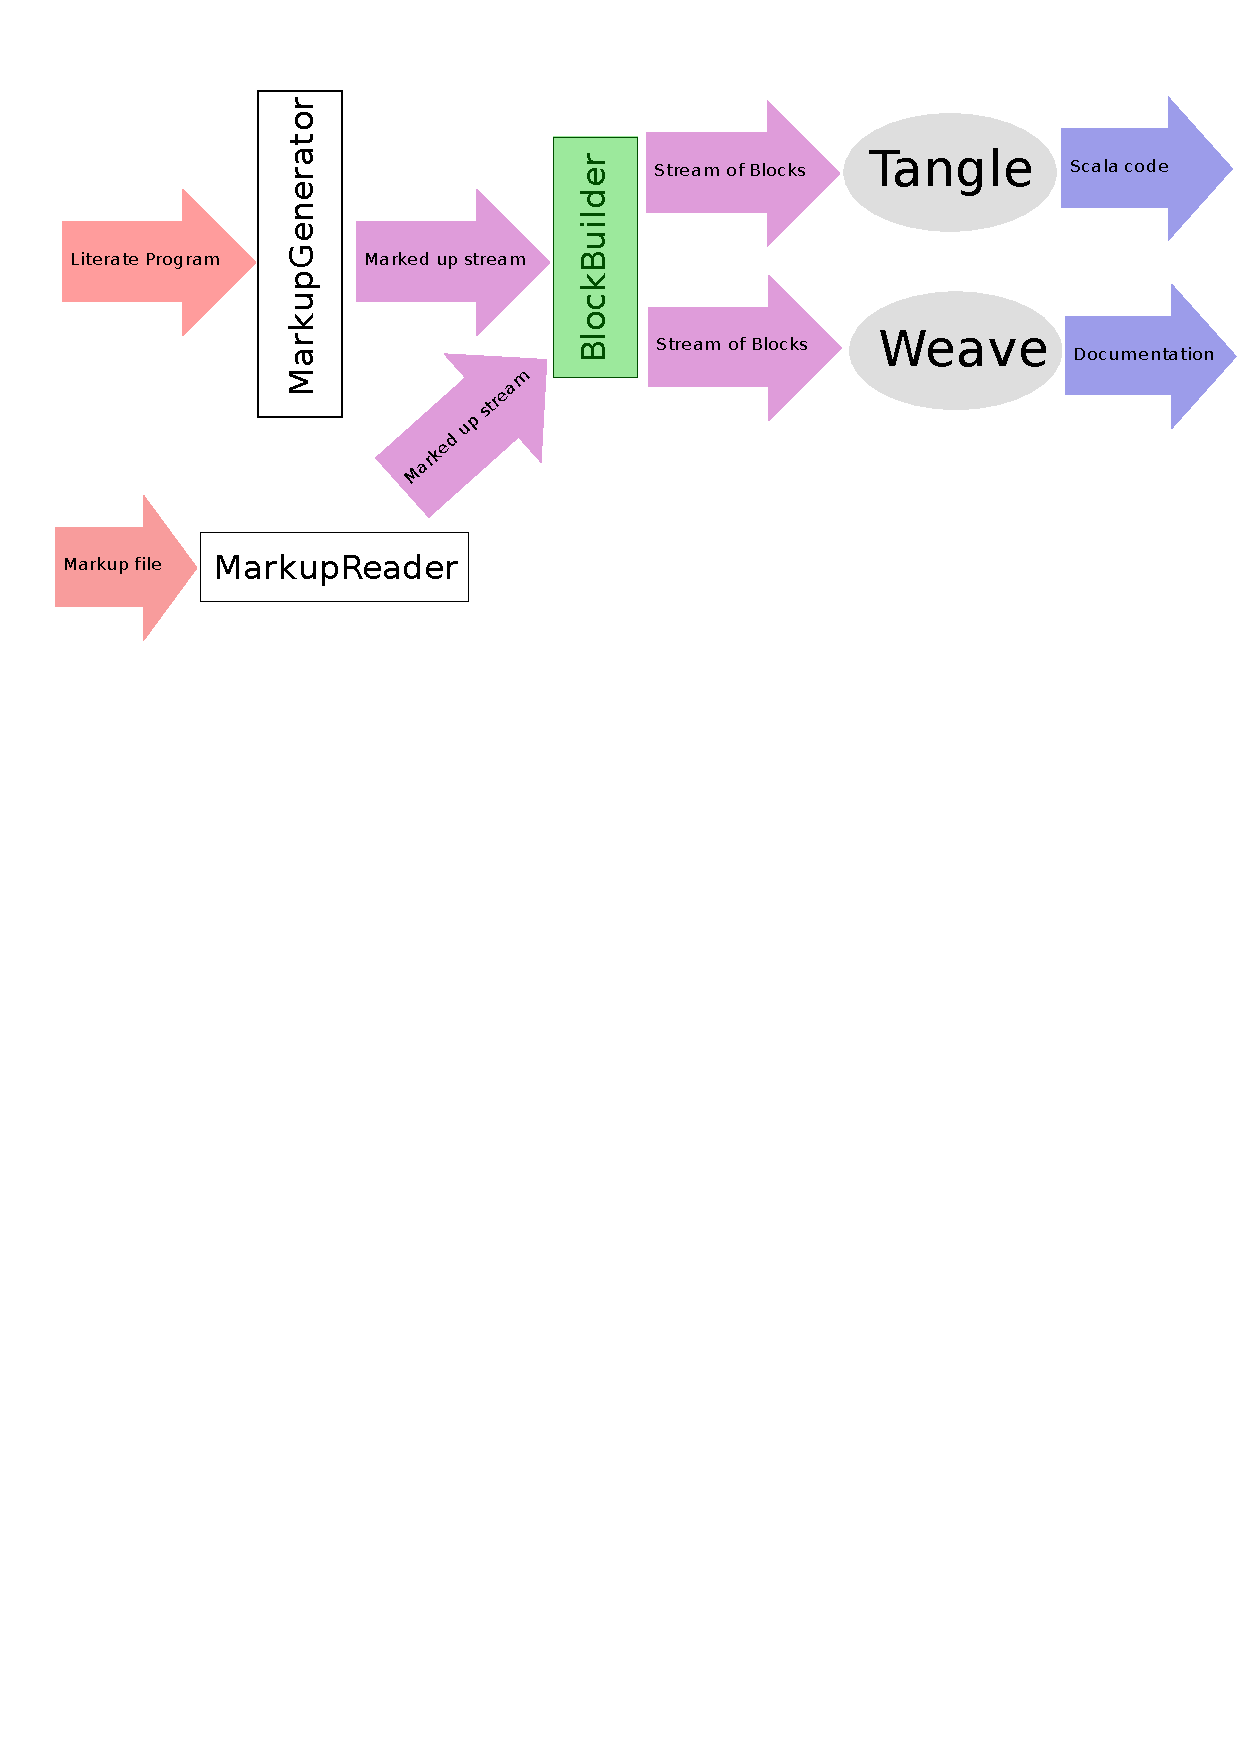
\includegraphics[width=10cm,viewport=167 590 508 800,clip]{images/blockBuilder}

$\left<\mbox{\emph{*}}\right>+\equiv$
\begin{program}{\vem package}~scalit.markup
\\[0.5em]$<$Combining~strings~and~references$>$
\\[0.5em]$<$The~block~format$>$
\\[0.5em]$<$Build~blocks$>$
\\[0.5em]$<$Test~the~block~format$>$
\\[0.5em]\end{program}
\subsection{The block format}
The aim of the block format is to store the information associated with a block
(their name, chunk number, line number) while providing easy access to the
string representation their content for weave. The only thing common between
code and documentation blocks are:

\begin{itemize}
\item Block number
\item Beginning line number
\end{itemize}

$\left<\mbox{\emph{The block format}}\right>\equiv$
\begin{program}{\vem sealed}~{\vem abstract}~{\vem class}~Block$($blocknumber\,{\rm :}~Int,~linenumber\,{\rm :}~Int,
\\~~~~~~~~~~~~~~~~~~~~~~~~~~~~~~~~~~~~~~~~~~~~~~~~~~~~~~~~content\,{\rm :}~Stream$[$Line$]$$)$~{\small\{}
\\~~~~~~$<$body~of~the~block~{\vem class}$>$
\\{\small\}}
\\[0.5em]\end{program}
For the string representation, we run into a problem: While during tangling
we want to extract references to other code blocks, this is not the case
when we want to create documentation: Here we only want to see the name.
Another problem arises with quoted strings (that occur in documentation blocks):
Their content will be output verbatim in the documentation and deserves another
treatment. The solution here is to have a stream that can contain either
strings, references to other blocks or quoted strings.

$\left<\mbox{\emph{Combining strings and references}}\right>\equiv$
\begin{program}{\vem object}~StringRefs~{\small\{}
\\~~~~{\vem sealed}~{\vem abstract}~{\vem class}~StringRef
\\~~~~{\vem case}~{\vem class}~RealString$($content\,{\rm :}~String,
\\~~~~~~~~~~~~~~~~~~~~~~~~~~~~~~~~~~~~from\,{\rm :}~Int,
\\~~~~~~~~~~~~~~~~~~~~~~~~~~~~~~~~~~~~to\,{\rm :}~Int$)$~{\vem extends}~StringRef
\\~~~~{\vem case}~{\vem class}~QuotedString$($content\,{\rm :}~String$)$~{\vem extends}~StringRef
\\~~~~{\vem case}~{\vem class}~BlockRef$($referenced\,{\rm :}~CodeBlock$)$~{\vem extends}~StringRef
\\[0.5em]~~~~{\vem implicit}~{\vem def}~realString2string$($rs\,{\rm :}~RealString$)$~=~rs.content
\\{\small\}}
\\[0.5em]\end{program}
With these three different contents, we are able to define a method
that, given a map of code blocks (for dereference) will give us a
stream of \texttt{StringRef}:

$\left<\mbox{\emph{body of the block class}}\right>\equiv$
\begin{program}{\vem import}~StringRefs.\_
\\[0.5em]{\vem def}~stringRefForm$($codeBlocks\,{\rm :}~Map$[$String,CodeBlock$]$$)${\rm :}~Stream$[$StringRef$]$
\\[0.5em]\end{program}
\subsubsection{Code blocks}
With this class, we can now represent the content of code blocks.
One special field is the reference to the next block: We will not
know this in the beginning, but when everything is read in, it
can be calculated.

Given a map of code blocks and their associated name, we can also
easily give back the stream of \texttt{StringRef}s:

$\left<\mbox{\emph{The block format}}\right>+\equiv$
\begin{program}{\vem case}~{\vem class}~CodeBlock$($blocknumber\,{\rm :}~Int,~linenumber\,{\rm :}~Int,
\\~~~~~~~~~~content\,{\rm :}~Stream$[$Line$]$,~blockname\,{\rm :}~String$)$
\\~~~~~~~~~~~~~~{\vem extends}~Block$($blocknumber,linenumber,content$)$~{\small\{}
\\~~~~{\vem import}~StringRefs.\_
\\~~~~{\vem override}~{\vem def}~stringRefForm$($
\\~~~~~~~~codeBlocks\,{\rm :}~Map$[$String,CodeBlock$]$$)${\rm :}~Stream$[$StringRef$]$~=~{\small\{}
\\[0.5em]\end{program}
This is done by accumulating the string as long as we do not have
a reference. When a reference occurs, we terminate the current string
part and intersperse a use name. In parallel, we'll have to store the
offset inside the code block as to know which lines the string reference
represents:

$\left<\mbox{\emph{The block format}}\right>+\equiv$
\begin{program}~~~~{\vem def}~cbAcc$($ls\,{\rm :}~Stream$[$Line$]$,~acc\,{\rm :}~String,
\\~~~~~~~~~~~~~~~~begin\,{\rm :}~Int,~off\,{\rm :}~Int$)${\rm :}~Stream$[$StringRef$]$~=
\\ls~{\vem match}~{\small\{}
\\~~~~{\vem case}~Stream.cons$($first,rest$)$~$\Rightarrow$~first~{\vem match}~{\small\{}
\\~~~~~~~~{\vem case}~NewLine~$\Rightarrow$~cbAcc$($rest,~acc~$+$~"$\backslash$n",~begin,~off~$+$~1$)$
\\~~~~~~~~{\vem case}~TextLine$($content$)$~$\Rightarrow$
\\~~~~~~~~~~~~cbAcc$($rest,~acc~$+$~content,~begin,~off$)$
\\~~~~~~~~{\vem case}~Use$($usename$)$~$\Rightarrow$~{\small\{}
\\~~~~~~~~~~~~{\vem val}~cb~=~codeBlocks~get~usename~{\vem match}~{\small\{}
\\~~~~~~~~~~~~~~~~{\vem case}~Some$($codeBlock$)$~$\Rightarrow$~codeBlock
\\~~~~~~~~~~~~~~~~{\vem case}~None~$\Rightarrow$
\\~~~~~~~~~~~~~~~~~~~~System.err.println$($"Did~not~find~block~"~$+$
\\~~~~~~~~~~~~~~~~~~~~~~~~~~~~~~~~~~~~~~~~~~~~~~~~~~usename$)$
\\~~~~~~~~~~~~~~~~~~~~exit$($1$)$
\\~~~~~~~~~~~~{\small\}}
\\~~~~~~~~~~~~Stream.cons$($RealString$($acc,begin,off$)$,
\\~~~~~~~~~~~~Stream.cons$($BlockRef$($cb$)$,cbAcc$($rest,"",off,off$)$$)$$)$
\\~~~~~~~~{\small\}}
\\~~~~~~~~{\vem case}~other~$\Rightarrow$~error$($"Unexpected~line\,{\rm :}~"~$+$~other$)$
\\~~~~{\small\}}
\\[0.5em]\end{program}
We will also have to handle the case where we are finished with reading.
Nothing special here.

$\left<\mbox{\emph{The block format}}\right>+\equiv$
\begin{program}~~~~{\vem case}~Stream.empty~$\Rightarrow$~acc~{\vem match}~{\small\{}
\\~~~~~~~~{\vem case}~""~$\Rightarrow$~Stream.empty
\\~~~~~~~~{\vem case}~s~~$\Rightarrow$~Stream.cons$($RealString$($s,begin,off$)$,Stream.empty$)$
\\~~~~{\small\}}
\\{\small\}}
\\~~~~~~~~~~~~
\\~~~~cbAcc$($content,"",linenumber,linenumber$)$
\\~~~~{\small\}}
\\{\small\}}
\\[0.5em]\end{program}
\subsubsection{Documentation blocks}
For documentation blocks, we do not have to take care of eventual references.
However, quoted blocks will need to be identified.

$\left<\mbox{\emph{The block format}}\right>+\equiv$
\begin{program}{\vem case}~{\vem class}~DocuBlock$($blocknumber\,{\rm :}~Int,~linenumber\,{\rm :}~Int,
\\content\,{\rm :}~Stream$[$Line$]$$)$~{\vem extends}
\\~~~~Block$($blocknumber,linenumber,content$)$~{\small\{}
\\~~~~{\vem import}~StringRefs.\_
\\~~~~{\vem override}~{\vem def}~stringRefForm$($codeBlocks\,{\rm :}~Map$[$String,CodeBlock$]$$)${\rm :}
\\~~~~~~~~Stream$[$StringRef$]$~=~{\small\{}
\\~~~~~~~~~~~~srContent
\\~~~~~~~~{\small\}}
\\~~~~$<$define~the~string~content~value$>$
\\{\small\}}
\\[0.5em]\end{program}
Because we do not really depend on the code Blocks, we will be able
to lazily initialize a value holding the whole Stream. At the moment,
we'll not even store the line numbers of documentation: What for?

$\left<\mbox{\emph{define the string content value}}\right>\equiv$
\begin{program}~~~~{\vem lazy}~{\vem val}~srContent\,{\rm :}~Stream$[$StringRef$]$~=~{\small\{}
\\~~~~~~~~{\vem def}~srcAcc$($ls\,{\rm :}~Stream$[$Line$]$,~acc\,{\rm :}~String$)${\rm :}~Stream$[$StringRef$]$~=
\\~~~~~~~~~~~~ls~{\vem match}~{\small\{}
\\~~~~~~~~~~~~~~~~{\vem case}~Stream.empty~$\Rightarrow$
\\~~~~~~~~~~~~~~~~~~~~Stream.cons$($RealString$($acc,$-$1,$-$1$)$,
\\~~~~~~~~~~~~~~~~~~~~Stream.empty$)$
\\~~~~~~~~~~~~~~~~{\vem case}~Stream.cons$($first,rest$)$~$\Rightarrow$~first~{\vem match}~{\small\{}
\\~~~~~~~~~~~~~~~~~~~~{\vem case}~NewLine~$\Rightarrow$~srcAcc$($rest,acc~$+$~"$\backslash$n"$)$
\\~~~~~~~~~~~~~~~~~~~~{\vem case}~TextLine$($content$)$~$\Rightarrow$~srcAcc$($rest,~acc~$+$~content$)$
\\[0.5em]\end{program}
Like in the code case, these two are relatively trivial. We will need
to invoke another function for quotes.

$\left<\mbox{\emph{define the string content value}}\right>+\equiv$
\begin{program}{\vem case}~Quote~$\Rightarrow$~{\small\{}
\\~~~~{\vem val}~$($quoted,continue$)$~=~quote$($rest,""$)$
\\~~~~Stream.cons$($RealString$($acc,$-$1,$-$1$)$,
\\~~~~Stream.cons$($quoted,srcAcc$($continue,""$)$$)$$)$
\\{\small\}}
\\{\vem case}~other~$\Rightarrow$~error$($"Unexpected~line~in~doc\,{\rm :}~"~$+$~other$)$
\\~~~~~~~~{\small\}}
\\~~~~{\small\}}
\\[0.5em]~~~~~~$<$quote~accumulation$>$
\\~~~~~~~~
\\~~~~~~srcAcc$($content,""$)$
\\{\small\}}
\\[0.5em]\end{program}
We still need the quote accumulation: Until the end of the quote, we
will just concatenate the string and then return where to continue and
the content:

$\left<\mbox{\emph{quote accumulation}}\right>\equiv$
\begin{program}{\vem def}~quote$($ls\,{\rm :}~Stream$[$Line$]$,
\\~~~~~~~~~~~~acc\,{\rm :}~String$)${\rm :}~$($QuotedString,Stream$[$Line$]$$)$~=
\\~~~~ls~{\vem match}~{\small\{}
\\~~~~~~~~{\vem case}~Stream.empty~$\Rightarrow$~$($QuotedString$($acc$)$,Stream.empty$)$
\\~~~~~~~~{\vem case}~Stream.cons$($first,rest$)$~$\Rightarrow$~first~{\vem match}~{\small\{}
\\~~~~~~~~~~~~{\vem case}~NewLine~$\Rightarrow$~quote$($rest,~acc~$+$~"$\backslash$n"$)$
\\~~~~~~~~~~~~{\vem case}~TextLine$($content$)$~$\Rightarrow$~quote$($rest,~acc~$+$~content$)$
\\~~~~~~~~~~~~{\vem case}~EndQuote~$\Rightarrow$~$($QuotedString$($acc$)$,rest$)$
\\~~~~~~~~~~~~{\vem case}~other~$\Rightarrow$~error$($"Unexpected~inside~quote\,{\rm :}~"~$+$~other$)$
\\~~~~~~~~{\small\}}
\\~~~~{\small\}}
\\[0.5em]\end{program}
\subsection{Building blocks}
The final document will consist of a number of blocks as defined above,
so the next step will be to parse these blocks. We will define a
block builder class like this:

$\left<\mbox{\emph{Build blocks}}\right>\equiv$
\begin{program}{\vem case}~{\vem class}~BlockBuilder$($lines\,{\rm :}~Stream$[$Line$]$$)$~{\small\{}
\\~~~~{\vem def}~blocks\,{\rm :}~Stream$[$Block$]$~=~lines~{\vem match}~{\small\{}
\\~~~~~~~~{\vem case}~Stream.cons$($\_,beg~@~Stream.cons$($Doc$($0$)$,\_$)$$)$~$\Rightarrow$~{\small\{}
\\~~~~~~~~~~~~selectNext$($beg,0$)$
\\~~~~~~~~{\small\}}
\\~~~~~~~~{\vem case}~\_~$\Rightarrow$~error$($"Unexpected~beginnig\,{\rm :}~"~$+$~lines.take$($2$)$.toList$)$
\\~~~~{\small\}}
\\[0.5em]\end{program}
The filename has to be extracted separately because it will not
be part of any block.

$\left<\mbox{\emph{Build blocks}}\right>+\equiv$
\begin{program}~~~~{\vem def}~filename\,{\rm :}~String~=~lines.head~{\vem match}~{\small\{}
\\~~~~~~~~{\vem case}~File$($fname$)$~$\Rightarrow$~fname
\\~~~~~~~~{\vem case}~other~$\Rightarrow$~error$($"Unexpected~first~line\,{\rm :}~"~$+$~other$)$
\\~~~~{\small\}}
\\[0.5em]~~~~$<$define~how~to~read~up~to~a~line~{\vem type}$>$
\\~~~~$<$define~documentation~and~code~splitting$>$
\\{\small\}}
\\[0.5em]\end{program}
Basicall, documentation and code splitting use one common part:
Read up to \texttt{EndCode} or \texttt{EndLine}, all while incrementing line
numbers. This functionality can be extracted:

$\left<\mbox{\emph{define how to read up to a line type}}\right>\equiv$
\begin{program}~~~~{\vem def}~readUpToTag$($ls\,{\rm :}~Stream$[$Line$]$,
\\~~~~~~~~~~~~~~~~~~~~~~~~~~~~~~~~~~~~acc\,{\rm :}~Stream$[$Line$]$,
\\~~~~~~~~~~~~~~~~~~~~~~~~~~~~~~~~~~~~linenumber\,{\rm :}~Int,
\\~~~~~~~~~~~~~~~~~~~~~~~~~~~~~~~~~~~~endTag\,{\rm :}~Line$)${\rm :}
\\~~~~~~~~$($Stream$[$Line$]$,Stream$[$Line$]$,Int$)$~=~ls~{\vem match}~{\small\{}
\\~~~~~~~~~~~~{\vem case}~Stream.empty~$\Rightarrow$
\\~~~~~~~~~~~~~~~~error$($"Expected~end~tag~but~found~end~of~stream"$)$
\\~~~~~~~~~~~~{\vem case}~Stream.cons$($first,rest$)$~$\Rightarrow$
\\~~~~~~~~~~~~~~~~{\vem if}$($~first~$==$~endTag~$)$
\\~~~~~~~~~~~~~~~~~~~~$($acc.reverse,rest,linenumber$)$
\\~~~~~~~~~~~~~~~~{\vem else}~first~{\vem match}~{\small\{}
\\~~~~~~~~~~~~~~~~~~~~{\vem case}~NewLine~$\Rightarrow$
\\~~~~~~~~~~~~~~~~~~~~~~~~readUpToTag$($rest,
\\~~~~~~~~~~~~~~~~~~~~~~~~~~~~Stream.cons$($first,acc$)$,
\\~~~~~~~~~~~~~~~~~~~~~~~~~~~~linenumber~$+$~1,endTag$)$
\\~~~~~~~~~~~~~~~~~~~~{\vem case}~other~$\Rightarrow$
\\~~~~~~~~~~~~~~~~~~~~~~~~readUpToTag$($rest,
\\~~~~~~~~~~~~~~~~~~~~~~~~~~~~Stream.cons$($first,acc$)$,
\\~~~~~~~~~~~~~~~~~~~~~~~~~~~~linenumber,endTag$)$
\\~~~~~~~~~~~~~~~~{\small\}}
\\~~~~{\small\}}
\\[0.5em]\end{program}
This would be quite a bit more flexible if we could just check for
a specific type, but somehow erasure prevents me from doing that.

The real work will be done with the two methods, documentation and
code (which will call one another via \texttt{selectNext}): They split the
content along the lines. First the function selectNext:

$\left<\mbox{\emph{define documentation and code splitting}}\right>\equiv$
\begin{program}~~~~{\vem def}~selectNext$($ls\,{\rm :}~Stream$[$Line$]$,
\\~~~~~~~~~~~~~~~~~~~~~~~~~~~~~~~~~~linenumber\,{\rm :}~Int$)${\rm :}~Stream$[$Block$]$~=
\\~~~~~~~~ls~{\vem match}~{\small\{}
\\~~~~~~~~~~~~{\vem case}~Stream.empty~$\Rightarrow$~Stream.empty
\\~~~~~~~~~~~~{\vem case}~Stream.cons$($first,rest$)$~$\Rightarrow$~first~{\vem match}~{\small\{}
\\~~~~~~~~~~~~~~~~{\vem case}~Doc$($n$)$~$\Rightarrow$~documentation$($rest,n,linenumber$)$
\\~~~~~~~~~~~~~~~~{\vem case}~Code$($n$)$~$\Rightarrow$~code$($rest,n,linenumber$)$
\\~~~~~~~~~~~~~~~~{\vem case}~other~$\Rightarrow$~error$($"Expected~begin~code~or~begin~doc"~$+$
\\~~~~~~~~~~~~~~~~~~~~~~~~~~~~~~~~~~~~~~~~~~~~~~~~~~~~~~~~"but~found~"~$+$~other$)$
\\~~~~~~~~~~~~{\small\}}
\\~~~~~~~~{\small\}}
\\[0.5em]\end{program}
Nothing too spectacular here. For documentation, we will pass everything
up to \texttt{EndDoc(n)} to \texttt{DocuBlock}.

$\left<\mbox{\emph{define documentation and code splitting}}\right>+\equiv$
\begin{program}~~~~{\vem def}~documentation$($ls\,{\rm :}~Stream$[$Line$]$,
\\~~~~~~~~~~~~~~~~~~~~~~~~~~~~~~~~~~~~~~~~blocknumber\,{\rm :}~Int,
\\~~~~~~~~~~~~~~~~~~~~~~~~~~~~~~~~~~~~~~~~linenumber\,{\rm :}~Int$)${\rm :}~Stream$[$Block$]$~=
\\~~~~~~~~{\small\{}
\\[0.5em]\end{program}
With the function readUpToTag, this becomes quite simple:

$\left<\mbox{\emph{define documentation and code splitting}}\right>+\equiv$
\begin{program}ls~{\vem match}~{\small\{}
\\~~~~{\vem case}~Stream.empty~$\Rightarrow$~error$($"Unexpected~empty~doc~block"$)$
\\~~~~{\vem case}~s~@~Stream.cons$($first,rest$)$~$\Rightarrow$~{\small\{}
\\~~~~~~~~{\vem val}~$($blockLines,cont,nextline$)$~=
\\~~~~~~~~readUpToTag$($s,Stream.empty,linenumber,EndDoc$($blocknumber$)$$)$
\\~~~~~~~~Stream.cons$($
\\~~~~~~~~DocuBlock$($blocknumber,
\\~~~~~~~~~~~~~~~~~~~~~~~~~~~~linenumber,
\\~~~~~~~~~~~~~~~~~~~~~~~~~~~~blockLines$)$,
\\~~~~~~~~~~selectNext$($cont,nextline$)$$)$
\\~~~~~~{\small\}}
\\~~{\small\}}
\\{\small\}}
\\[0.5em]\end{program}
The code splitting will work in exactly the same way, but we have to
take care of another element: The name of the code block.

$\left<\mbox{\emph{define documentation and code splitting}}\right>+\equiv$
\begin{program}~~~~{\vem def}~code$($ls\,{\rm :}~Stream$[$Line$]$,
\\~~~~~~~~~~~~~~~~~~~~~~blocknumber\,{\rm :}~Int,
\\~~~~~~~~~~~~~~~~~~~~~~linenumber\,{\rm :}~Int$)${\rm :}~Stream$[$Block$]$~=~{\small\{}
\\[0.5em]\end{program}
The format requires that the first element inside a code block is
the chunk name that is defined. Also, we eat the newline that comes
directly after that. Because we eat this, we'll also have to update
the information on from which line we actually have content.

$\left<\mbox{\emph{define documentation and code splitting}}\right>+\equiv$
\begin{program}~~~~~~~~~~~~{\vem val}~Stream.cons$($defline,Stream.cons$($nline,cont$)$$)$~=~ls
\\~~~~~~~~~~~~{\vem val}~chunkname~=~defline~{\vem match}~{\small\{}
\\~~~~~~~~~~~~~~~~{\vem case}~Definition$($name$)$~$\Rightarrow$~name
\\~~~~~~~~~~~~~~~~{\vem case}~other~$\Rightarrow$~error$($"Expected~definition~but~got~"~$+$~other$)$
\\~~~~~~~~~~~~{\small\}}
\\~~~~~~~~~~~~{\vem val}~cont2~=~nline~{\vem match}~{\small\{}
\\~~~~~~~~~~~~~~~~{\vem case}~NewLine~$\Rightarrow$~cont
\\~~~~~~~~~~~~~~~~{\vem case}~\_~$\Rightarrow$~Stream.cons$($nline,cont$)$
\\~~~~~~~~~~~~{\small\}}
\\~~~~~~~~~~~~{\vem val}~linenumber2~=~linenumber~$+$~1
\\[0.5em]\end{program}
 With this information, we can accumulate the content:

$\left<\mbox{\emph{define documentation and code splitting}}\right>+\equiv$
\begin{program}~~~~~~~~ls~{\vem match}~{\small\{}
\\~~~~~~~~~~~~{\vem case}~Stream.empty~$\Rightarrow$~error$($"Unexpected~empty~code~block"$)$
\\~~~~~~~~~~~~{\vem case}~Stream.cons$($first,rest$)$~$\Rightarrow$
\\~~~~~~~~~~~~~~~~{\vem val}~$($lines,continue,lnumber$)$~=
\\~~~~~~~~~~~~~~~~~~~~readUpToTag$($cont2,Stream.empty,
\\~~~~~~~~~~~~~~~~~~~~~~~~~~~~~~~~~~~~~~~~~~~~linenumber2,EndCode$($blocknumber$)$$)$
\\[0.5em]~~~~~~~~~~~~Stream.cons$($
\\~~~~~~~~~~~~~~~~CodeBlock$($blocknumber,
\\~~~~~~~~~~~~~~~~~~~~~~~~~~~~~~~~~~~~linenumber2,
\\~~~~~~~~~~~~~~~~~~~~~~~~~~~~~~~~~~~~lines,
\\~~~~~~~~~~~~~~~~~~~~~~~~~~~~~~~~~~~~chunkname$)$,selectNext$($continue,lnumber$)$$)$
\\~~~~~~~~{\small\}}
\\~~~~{\small\}}
\\[0.5em]\end{program}
\subsection{Testing the block format}
The following application will read in a literate program and output
each element of the stream of blocks.

$\left<\mbox{\emph{Test the block format}}\right>\equiv$
\begin{program}{\vem object}~Blocks~{\small\{}
\\~~~~{\vem def}~usage\,{\rm :}~Unit~=~{\small\{}
\\~~~~~~~~System.err.println$($"Usage\,{\rm :}~scala~markup.Blocks~$[$infile$]$$\backslash$n"$)$
\\~~~~{\small\}}
\\[0.5em]~~~~{\vem def}~main$($args\,{\rm :}~Array$[$String$]$$)$~=~{\small\{}
\\~~~~~~~~{\vem import}~util.conversions.\_
\\[0.5em]~~~~~~~~{\vem val}~blocks~=~args.length~{\vem match}~{\small\{}
\\~~~~~~~~~~~~{\vem case}~0~$\Rightarrow$~blocksFromLiterateInput$($System.in$)$
\\~~~~~~~~~~~~{\vem case}~1~$\Rightarrow$~blocksFromLiterateFile$($args$($0$)$$)$
\\~~~~~~~~~~~~{\vem case}~\_~$\Rightarrow$~usage;~exit
\\~~~~~~~~{\small\}}
\\[0.5em]~~~~~~~~blocks~foreach~{\small\{}
\\~~~~~~~~~~~~b~$\Rightarrow$~println$($b$)$
\\~~~~~~~~{\small\}}
\\~~~~{\small\}}
\\{\small\}}
\end{program}
\section{How to extract source code from a literate program}
\texttt{tangle} is the tool that extracts source code from a given literate
program. For this extraction, we base ourselves on the stream of blocks
generated in the file \texttt{markup/blocks.nw}

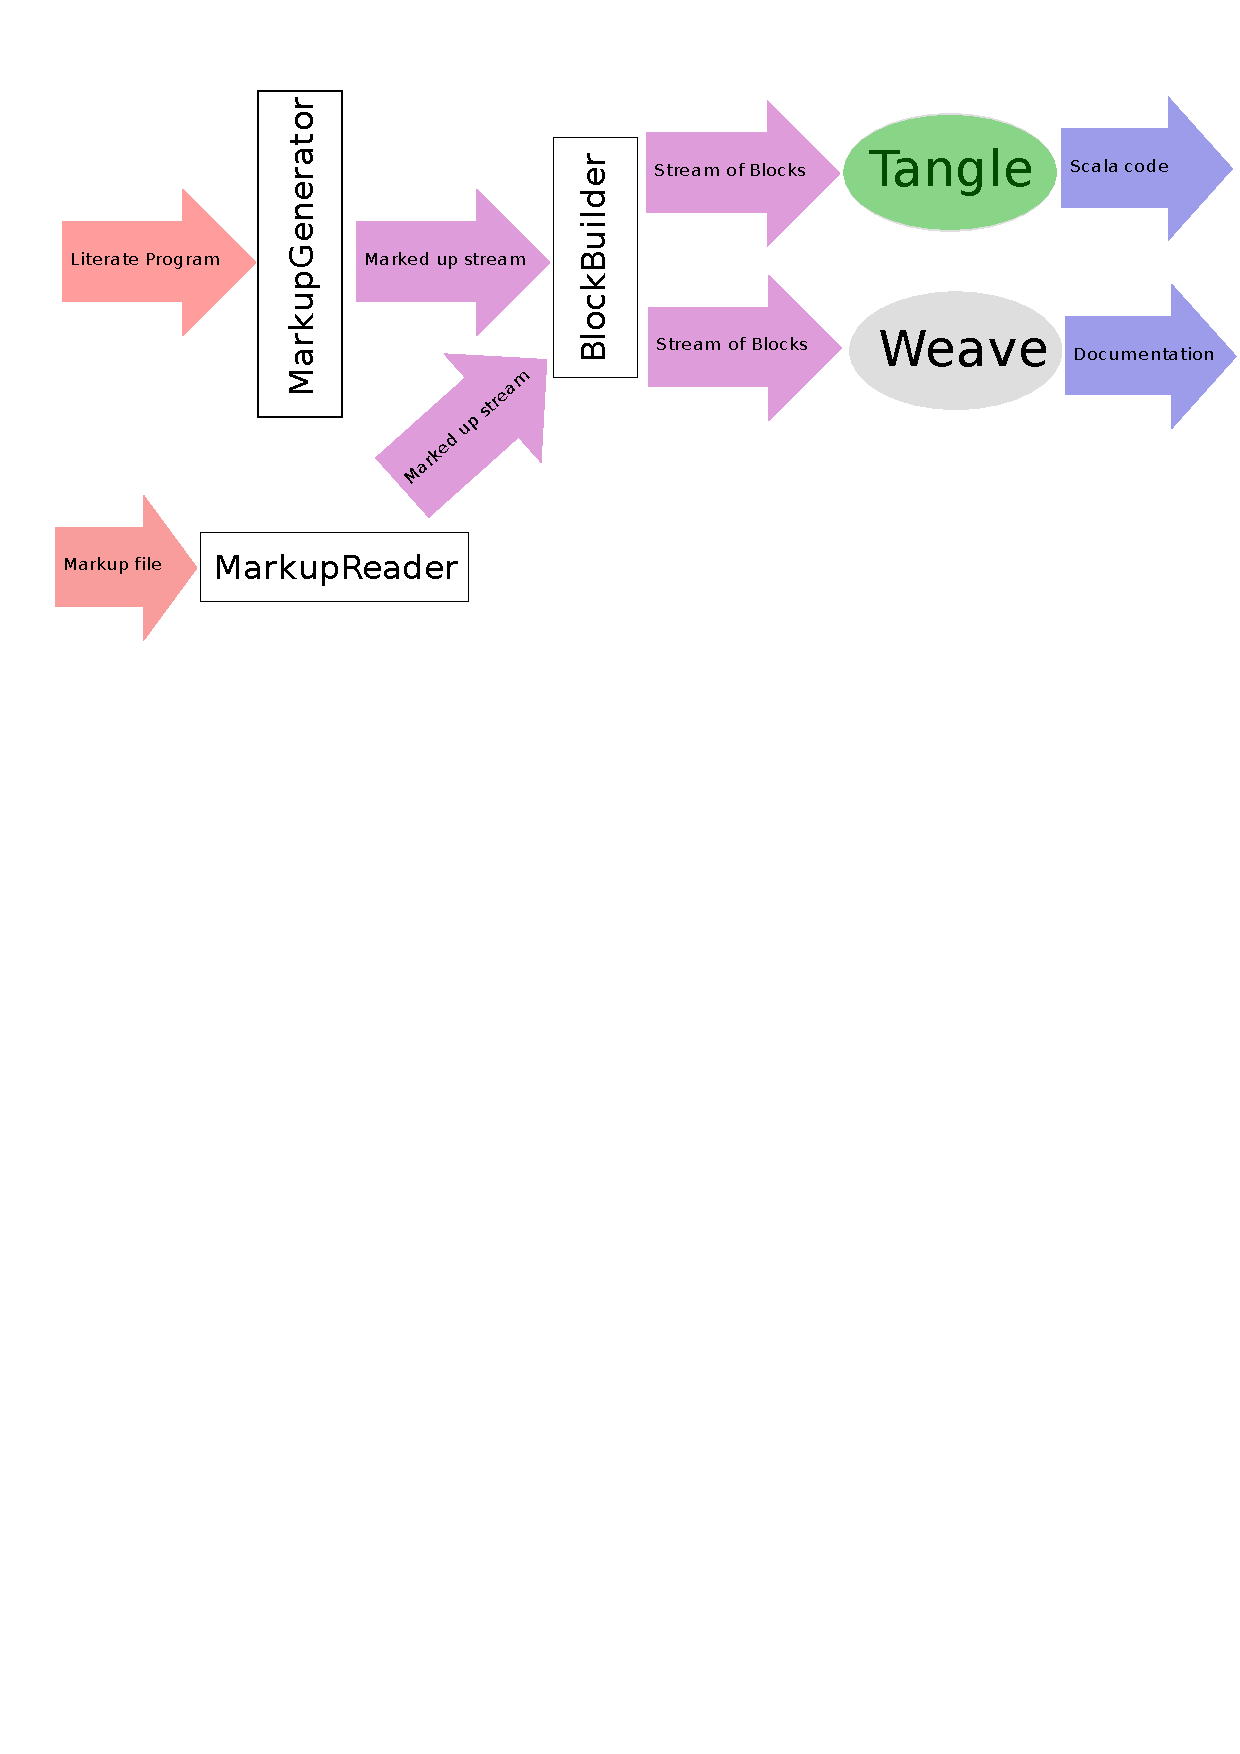
\includegraphics[width=10cm,viewport=310 710 600 800,clip]{images/tangle}

\subsection{Overview}
Tangle will first extract a map of code blocks, from which it will
output the sources in the right format the routines for output are
directly associated with the map and will be explained in section
\ref{puzzle}.

$\left<\mbox{\emph{*}}\right>+\equiv$
\begin{program}{\vem package}~scalit.tangle
\\{\vem import}~markup.\_
\\[0.5em]$<$code~chunks$>$
\\[0.5em]$<$puzzle~code~chunks~together$>$
\\[0.5em]$<$output~the~source$>$
\\[0.5em]\end{program}
\label{puzzle}\subsection{Puzzling code blocks together}
\subsubsection{Code chunks}
While the block generator already provides us with a stream of
blocks, several of these might be describing the same code chunk.
So a pointer to the next code block describing this chunk has to be
provided. We do this using an \texttt{Option}:

$\left<\mbox{\emph{code chunks}}\right>\equiv$
\begin{program}{\vem case}~{\vem class}~CodeChunk$($bn\,{\rm :}~Int,~ln\,{\rm :}~Int,
\\~~~~~~~~~~~~~~~~~~~~~~cont\,{\rm :}~Stream$[$Line$]$,bname\,{\rm :}~String,
\\~~~~~~~~~~~~~~~~~~~~~~next\,{\rm :}~Option$[$CodeChunk$]$$)$~{\vem extends}
\\CodeBlock$($bn,ln,cont,bname$)$~{\small\{}
\\~~~~
\\~~~~{\vem import}~StringRefs.\_
\\[0.5em]\end{program}
The append method will be useful when we will actually construct
the chunks.

$\left<\mbox{\emph{code chunks}}\right>+\equiv$
\begin{program}~~~~{\vem def}~append$($that\,{\rm :}~CodeBlock$)${\rm :}~CodeChunk~=~next~{\vem match}~{\small\{}
\\~~~~~~~~{\vem case}~None~$\Rightarrow$
\\~~~~~~~~~~~~CodeChunk$(${\vem this}.blocknumber,
\\~~~~~~~~~~~~~~~~~~~~~~~~~~~~~~~~{\vem this}.linenumber,
\\~~~~~~~~~~~~~~~~~~~~~~~~~~~~~~~~{\vem this}.content,
\\~~~~~~~~~~~~~~~~~~~~~~~~~~~~~~~~{\vem this}.blockname,
\\~~~~~~~~~~~~~~~~~~~~~~~~~~~~~~~~Some$($CodeChunk$($that.blocknumber,
\\~~~~~~~~~~~~~~~~~~~~~~~~~~~~~~~~~~~~~~~~that.linenumber,
\\~~~~~~~~~~~~~~~~~~~~~~~~~~~~~~~~~~~~~~~~that.content,
\\~~~~~~~~~~~~~~~~~~~~~~~~~~~~~~~~~~~~~~~~that.blockname,None$)$$)$$)$
\\~~~~~~~~{\vem case}~Some$($next$)$~$\Rightarrow$
\\~~~~~~~~~~~~CodeChunk$(${\vem this}.blocknumber,
\\~~~~~~~~~~~~~~~~~~~~~~~~~~~~~~~~{\vem this}.linenumber,
\\~~~~~~~~~~~~~~~~~~~~~~~~~~~~~~~~{\vem this}.content,
\\~~~~~~~~~~~~~~~~~~~~~~~~~~~~~~~~{\vem this}.blockname,
\\~~~~~~~~~~~~~~~~~~~~~~~~~~~~~~~~Some$($next~append~that$)$$)$
\\~~~~{\small\}}
\\[0.5em]\end{program}
With this linked-list-like definition in place, we can also redefine
the string reference form by simply appending the output of the next
element:

$\left<\mbox{\emph{code chunks}}\right>+\equiv$
\begin{program}~~~~{\vem override}~{\vem def}~stringRefForm$($codeChunks\,{\rm :}~Map$[$String,CodeBlock$]$$)${\rm :}
\\~~~~~~~~Stream$[$StringRef$]$~=~next~{\vem match}~{\small\{}
\\~~~~~~~~~~~~{\vem case}~None~$\Rightarrow$~{\vem super}.stringRefForm$($codeChunks$)$
\\~~~~~~~~~~~~{\vem case}~Some$($el$)$~$\Rightarrow$~Stream.concat$($
\\~~~~~~~~~~~~~~~~{\vem super}.stringRefForm$($codeChunks$)$,
\\~~~~~~~~~~~~~~~~el.stringRefForm$($codeChunks$)$$)$
\\~~~~~~~~{\small\}}
\\{\small\}}
\\[0.5em]\end{program}
\subsubsection{A collection of chunks}
In a chunk collection, we accumulate chunks on in a map. Also
very important is the file name.

$\left<\mbox{\emph{puzzle code chunks together}}\right>\equiv$
\begin{program}{\vem import}~scala.collection.immutable.{\small\{}Map,HashMap{\small\}}
\\{\vem case}~{\vem class}~ChunkCollection$($cm\,{\rm :}~Map$[$String,CodeChunk$]$,
\\~~~~~~~~~~~~~~~~~~~~~~~~~~~~~~~~~~~~~~~~~~~~~~~~~~filename\,{\rm :}~String$)$~{\small\{}
\\[0.5em]~~~~{\vem import}~StringRefs.\_
\\[0.5em]\end{program}
To get the stream of code is now as simple as calling
serialize. Flatten will convert it to a string.

$\left<\mbox{\emph{puzzle code chunks together}}\right>+\equiv$
\begin{program}~~~~{\vem def}~serialize$($chunkname\,{\rm :}~String$)${\rm :}~String~=
\\~~~~~~~~cm~get~chunkname~{\vem match}~{\small\{}
\\~~~~~~~~~~~~{\vem case}~None~$\Rightarrow$~error$($"Did~not~find~chunk~"~$+$~chunkname$)$
\\~~~~~~~~~~~~{\vem case}~Some$($el$)$~$\Rightarrow$~flatten$($el.stringRefForm$($cm$)$$)$
\\~~~~~~~~{\small\}}
\\[0.5em]\end{program}
From the stream of blocks, we will receive the code blocks. We
will have to generate code chunks out of them.

$\left<\mbox{\emph{puzzle code chunks together}}\right>+\equiv$
\begin{program}~~~~{\vem def}~addBlock$($that\,{\rm :}~CodeBlock$)${\rm :}~ChunkCollection~=
\\~~~~~~~~cm~get~that.blockname~{\vem match}~{\small\{}
\\~~~~~~~~~~~~{\vem case}~None~$\Rightarrow$~ChunkCollection$($cm~$+$
\\~~~~~~~~~~~~~~~~$($that.blockname~$\rightarrow$
\\~~~~~~~~~~~~~~~~~~CodeChunk$($that.blocknumber,
\\~~~~~~~~~~~~~~~~~~~~~~~~~~~~~~~~~~~~that.linenumber,
\\~~~~~~~~~~~~~~~~~~~~~~~~~~~~~~~~~~~~that.content,
\\~~~~~~~~~~~~~~~~~~~~~~~~~~~~~~~~~~~~that.blockname,
\\~~~~~~~~~~~~~~~~~~~~~~~~~~~~~~~~~~~~None$)$$)$,filename$)$
\\~~~~~~~~~~~~{\vem case}~Some$($el$)$~$\Rightarrow$~ChunkCollection$($cm~$+$
\\~~~~~~~~~~~~~~~~$($that.blockname~$\rightarrow$
\\~~~~~~~~~~~~~~~~~~el.append$($that$)$$)$,filename$)$
\\~~~~~~~~{\small\}}
\\[0.5em]\end{program}
While adding one block is useful, we will want to do this
for a whole stream of blocks:

$\left<\mbox{\emph{puzzle code chunks together}}\right>+\equiv$
\begin{program}~~~~{\vem def}~addBlocks$($those\,{\rm :}~Stream$[$CodeBlock$]$$)${\rm :}~ChunkCollection~=
\\~~~~~~~~$($those~foldLeft~{\vem this}$)$~{\small\{}
\\~~~~~~~~~~~~$($acc\,{\rm :}~ChunkCollection,~n\,{\rm :}~CodeBlock$)$~$\Rightarrow$
\\~~~~~~~~~~~~~~~~acc.addBlock$($n$)$
\\~~~~~~~~{\small\}}
\\[0.5em]\end{program}
Finally, we'll have to define how to output a string containing the
whole code. In a first step, we'll have to expand references:

$\left<\mbox{\emph{puzzle code chunks together}}\right>+\equiv$
\begin{program}~~~~{\vem def}~expandRefs$($str\,{\rm :}~Stream$[$StringRef$]$$)${\rm :}~Stream$[$RealString$]$~=
\\~~~~~~~~str~{\vem match}~{\small\{}
\\~~~~~~~~~~~~{\vem case}~Stream.empty~$\Rightarrow$~Stream.empty
\\~~~~~~~~~~~~{\vem case}~Stream.cons$($first,rest$)$~$\Rightarrow$
\\~~~~~~~~~~~~~~~~first~{\vem match}~{\small\{}
\\~~~~~~~~~~~~~~~~~~~~{\vem case}~r~@~RealString$($\_,\_,\_$)$~$\Rightarrow$
\\~~~~~~~~~~~~~~~~~~~~~~~~Stream.cons$($r,expandRefs$($rest$)$$)$
\\~~~~~~~~~~~~~~~~~~~~{\vem case}~BlockRef$($ref$)$~$\Rightarrow$
\\~~~~~~~~~~~~~~~~~~~~~~~~Stream.concat$($
\\~~~~~~~~~~~~~~~~~~~~~~~~~~~~expandRefs$($cm$($ref.blockname$)$.stringRefForm$($cm$)$$)$,
\\~~~~~~~~~~~~~~~~~~~~~~~~~~~~expandRefs$($rest$)$$)$
\\~~~~~~~~~~~~~~~~~~~~{\vem case}~other~$\Rightarrow$~error$($"Unexpected~string~ref\,{\rm :}~"~$+$~other$)$
\\~~~~~~~~~~~~~~~~{\small\}}
\\~~~~~~~~{\small\}}
\\[0.5em]~~~~{\vem def}~expandedStream$($chunkname\,{\rm :}~String$)${\rm :}~Stream$[$RealString$]$~=
\\~~~~~~~~cm~get~chunkname~{\vem match}~{\small\{}
\\~~~~~~~~~~~~{\vem case}~None~$\Rightarrow$~error$($"Did~not~find~chunk~"~$+$~chunkname$)$
\\~~~~~~~~~~~~{\vem case}~Some$($el$)$~$\Rightarrow$~expandRefs$($el.stringRefForm$($cm$)$$)$
\\~~~~~~~~{\small\}}
\\[0.5em]\end{program}
After this expansion, the string form is quite easily made:

$\left<\mbox{\emph{puzzle code chunks together}}\right>+\equiv$
\begin{program}~~~~{\vem private}~{\vem def}~flatten$($str\,{\rm :}~Stream$[$StringRef$]$$)${\rm :}~String~=~{\small\{}
\\~~~~~~~~{\vem val}~sb~=~{\vem new}~StringBuffer
\\~~~~~~~~expandRefs$($str$)$~foreach~{\small\{}
\\~~~~~~~~~~~~{\vem case}~RealString$($content,\_,\_$)$~$\Rightarrow$~sb~append~content
\\~~~~~~~~{\small\}}
\\~~~~~~~~sb.toString
\\~~~~{\small\}}
\\{\small\}}
\\[0.5em]\end{program}
With the chunk collection logic in place, we will often have to access
to the empty chunk collection of a particular file name:

$\left<\mbox{\emph{puzzle code chunks together}}\right>+\equiv$
\begin{program}{\vem case}~{\vem class}~emptyChunkCollection$($fn\,{\rm :}~String$)$
\\~~~~~~~~~~{\vem extends}~ChunkCollection$($Map$($$)$,fn$)$
\\[0.5em]\end{program}
 \subsection{The main program}
With serialize defined, we can now accomplish the task of printing
the tangled source to standard output. Under \texttt{util/commandline.nw},
we defined a class for command line parsing that will be used here.
At the moment, we print out everything to standard output, one chunk
collection after another.

The following options can be given to tangle:

\begin{description}
\item[-r chunkname] Tries to extract the chunk with the name \texttt{chunkname}
\end{description}

$\left<\mbox{\emph{output the source}}\right>\equiv$
\begin{program}{\vem object}~Tangle~{\small\{}
\\~~~~{\vem def}~main$($args\,{\rm :}~Array$[$String$]$$)$~=~{\small\{}
\\~~~~~~~~{\vem import}~util.LiterateSettings
\\[0.5em]~~~~~~~~{\vem val}~ls~=~{\vem new}~LiterateSettings$($args$)$
\\[0.5em]~~~~~~~~{\vem val}~chunksToTake~=~ls.settings~get~"$-$r"~{\vem match}~{\small\{}
\\~~~~~~~~~~~~{\vem case}~None~$\Rightarrow$~Nil
\\~~~~~~~~~~~~{\vem case}~Some$($cs$)$~$\Rightarrow$~cs.reverse
\\~~~~~~~~{\small\}}
\\[0.5em]~~~~~~~~{\vem val}~out~=~ls.output
\\[0.5em]~~~~~~~~chunksToTake~{\vem match}~{\small\{}
\\~~~~~~~~~~~~{\vem case}~Nil~$\Rightarrow$
\\~~~~~~~~~~~~~~~~ls.chunkCollections~foreach~{\small\{}
\\~~~~~~~~~~~~~~~~~~~~cc~$\Rightarrow$~out.println$($cc.serialize$($"$*$"$)$$)$
\\~~~~~~~~~~~~~~~~{\small\}}
\\[0.5em]\end{program}
If we have specified some chunks to extract, we iterate over all the files
that we are given, extracting the specific chunk.

$\left<\mbox{\emph{output the source}}\right>+\equiv$
\begin{program}~~~~~~~~~~~~{\vem case}~cs~$\Rightarrow$
\\~~~~~~~~~~~~~~~~cs~foreach~{\small\{}
\\~~~~~~~~~~~~~~~~~~~~chunk~$\Rightarrow$
\\~~~~~~~~~~~~~~~~~~~~~~~~ls.chunkCollections~foreach~{\small\{}
\\~~~~~~~~~~~~~~~~~~~~~~~~~~~~cc~$\Rightarrow$
\\~~~~~~~~~~~~~~~~~~~~~~~~~~~~~~~~{\vem try}~{\small\{}
\\~~~~~~~~~~~~~~~~~~~~~~~~~~~~~~~~~~~~out.println$($cc.serialize$($chunk$)$$)$
\\~~~~~~~~~~~~~~~~~~~~~~~~~~~~~~~~{\small\}}~{\vem catch}~{\small\{}
\\~~~~~~~~~~~~~~~~~~~~~~~~~~~~~~~~~~~~{\vem case}~e~$\Rightarrow$~$($$)$
\\~~~~~~~~~~~~~~~~~~~~~~~~~~~~~~~~{\small\}}
\\~~~~~~~~~~~~~~~~~~~~~~~~{\small\}}
\\~~~~~~~~~~~~~~~~{\small\}}
\\~~~~~~~~{\small\}}
\\~~~~{\small\}}
\\{\small\}}
\end{program}
\section{A closer integration in the Scala compiler}
In the file \texttt{tangle.nw}, we outlined on how one could puzzle together a
compileable file out of a stream of blocks. This is very useful on its own,
but a closer compiler integration is desirable: This way, we can tell the
compiler the real line numbers of our literate program and not of the tangled
source - we will be able to debug more efficiently. Also, we can access
information provided by the compiler: What was defined by this block and
what variables will be used.

Concretely, we will be implementing \texttt{CoTangle} which will call the
compiler with the code taken from the stream of blocks. \texttt{LitComp} is
the command line application that directly compiles an input literate
program.

Additionally, we provide an object that directly exposes
\texttt{LiterateProgramSourceFiles}. This way, we can even use \texttt{scalac} to
work with literate programs.

$\left<\mbox{\emph{*}}\right>+\equiv$
\begin{program}{\vem package}~scalit.tangle
\\[0.5em]$<$CoTangle~$-$~send~tangled~to~compiler$>$
\\[0.5em]$<$A~source~file~format~{\vem for}~literate~programs$>$
\\[0.5em]$<$A~{\vem new}~position~{\vem type}$>$
\\[0.5em]$<$LitComp~$-$~the~command~line~application$>$
\\[0.5em]$<$LiterateCompilerSupport~$-$~{\vem object}~{\vem for}~scalac$>$
\\[0.5em]\end{program}
\subsection{CoTangle}
The following class will pass the source files that we get to the compiler (and
maybe a destination directory),
so a first step is to include the compiler class. Later, we'll outline
how to actually compile.

$\left<\mbox{\emph{CoTangle - send tangled to compiler}}\right>\equiv$
\begin{program}{\vem class}~CoTangle$($sourceFiles\,{\rm :}~List$[$LiterateProgramSourceFile$]$,
\\~~~~~~~~~~~~~~~~~~~~~~~~~~destination\,{\rm :}~Option$[$String$]$$)$~{\small\{}
\\~~~~$<$Include~a~compiler$>$
\\~~~~$<$Compile~a~literate~program$>$
\\{\small\}}
\\[0.5em]\end{program}
The compiler will also have to have a place to report errors to,
so we will need a reporter. The usual way would be to have an object
overriding some behavior for this, but we will just instantiate a
standard reporter.

$\left<\mbox{\emph{Include a compiler}}\right>\equiv$
\begin{program}~~~~{\vem import}~scala.tools.nsc.{\small\{}Global,Settings,reporters{\small\}}
\\~~~~{\vem import}~reporters.ConsoleReporter
\\[0.5em]\end{program}
At the moment, there is only one setting that we might give to the compiler:
If we have a destination directory, then we'll pass it

$\left<\mbox{\emph{Include a compiler}}\right>+\equiv$
\begin{program}~~~~{\vem val}~settings~=~{\vem new}~Settings$($$)$
\\~~~~destination~{\vem match}~{\small\{}
\\~~~~~~~~{\vem case}~Some$($dd$)$~$\Rightarrow$~{\small\{}
\\~~~~~~~~~~~~settings.outdir.tryToSet$($List$($"$-$d",dd$)$$)$
\\~~~~~~~~{\small\}}
\\~~~~~~~~{\vem case}~None~$\Rightarrow$~$($$)$
\\~~~~{\small\}}
\\~~~~{\vem val}~reporter~=
\\~~~~~~~~{\vem new}~ConsoleReporter$($settings,{\vem null},
\\~~~~~~~~~~~~~~~~~~~~~~~~~~~~~~~~~~~~~~~~~~~~~~~~{\vem new}~java.io.PrintWriter$($System.err$)$$)$
\\~~~~{\vem val}~compiler~=~{\vem new}~Global$($settings,reporter$)$
\\[0.5em]\end{program}
\subsection{Literate program as a source file}
After we have instanciated a compiler, we want to feed him a source
file. In this file, we'd like to conserve original line numbering etc.

Much of the functionality will be close to a batch source file. The main
thing that changes is the mapping position $\rightarrow$ position in literate
file.

$\left<\mbox{\emph{A source file format for literate programs}}\right>\equiv$
\begin{program}{\vem import}~scala.tools.nsc.util.{\small\{}BatchSourceFile,Position,LinePosition{\small\}}
\\{\vem class}~LiterateProgramSourceFile$($chunks\,{\rm :}~ChunkCollection$)$
\\~~~~{\vem extends}~BatchSourceFile$($chunks.filename,
\\~~~~~~~~~~~~~~~~~~~~~~~~~~~~~~~~~~~~~~~~~~~~~~~~~~~~chunks.serialize$($"$*$"$)$.toArray$)$~{\small\{}
\\~~~~$<$line~mappings$>$
\\~~~~$<$find~a~line$>$
\\~~~~$<$the~original~source~file$>$
\\~~~~$<$position~in~ultimate~source~file$>$
\\{\small\}}
\\[0.5em]\end{program}
\subsection{Position in ultimate source file}
The tangling process rearranges lines from the original literate program
so that they are a valid source input. For compiling purposes, we want to
find out to which original line a line in the tangled file corresponds. As
this will be done quite often, we want to cache the results:

$\left<\mbox{\emph{line mappings}}\right>\equiv$
\begin{program}~~~~{\vem val}~lines2orig~=~{\vem new}~scala.collection.mutable.HashMap$[$Int,Int$]$$($$)$
\\[0.5em]\end{program}
Finding a line amounts to iterating over the stream of code blocks until
we find the one containing the line. This might not be an optimal solution -
now that we are eating the first newline after the chunk definition, it
might actually happen that we point to the wrong line, for example with code
like 

\begin{verbatim}
val s = <Read s>
\end{verbatim}

and

\texttt{$\langle$$\langle$Read s$\rangle$$\rangle$=}
\begin{verbatim}
1/0
\end{verbatim}

Here, the error is in the second part of the code, but the line corresponding
to the first part will be returned. One way to fix this would be to consider
offset information.

$\left<\mbox{\emph{find a line}}\right>\equiv$
\begin{program}~~~~{\vem import}~scalit.markup.StringRefs.\_
\\~~~~{\vem lazy}~{\vem val}~codeblocks\,{\rm :}~Stream$[$RealString$]$~=
\\~~~~~~~~chunks.expandedStream$($"$*$"$)$
\\[0.5em]~~~~{\vem def}~findOrigLine$($ol\,{\rm :}~Int$)${\rm :}~Int~=
\\~~~~~~~~{\vem if}$($~lines2orig~contains~ol~$)$~lines2orig$($ol$)$
\\~~~~~~~~{\vem else}~{\small\{}
\\~~~~~~~~~~~~{\vem def}~find0$($offset\,{\rm :}~Int,
\\~~~~~~~~~~~~~~~~~~~~search\,{\rm :}~Stream$[$RealString$]$$)${\rm :}~Int~=~search~{\vem match}~{\small\{}
\\~~~~~~~~~~~~~~~~{\vem case}~Stream.empty~$\Rightarrow$~error$($"Could~not~find~line~{\vem for}~"~$+$~ol$)$
\\~~~~~~~~~~~~~~~~{\vem case}~Stream.cons$($first,rest$)$~$\Rightarrow$
\\~~~~~~~~~~~~~~~~~~~~first~{\vem match}~{\small\{}
\\~~~~~~~~~~~~~~~~~~~~~~~~{\vem case}~RealString$($cont,from,to$)$~$\Rightarrow$~{\small\{}
\\~~~~~~~~~~~~~~~~~~~~~~~~~~~~{\vem val}~diff~=~to~$-$~from
\\~~~~~~~~~~~~~~~~~~~~~~~~~~~~{\vem if}$($~ol~$\geq$~offset~\&\&~ol~$\leq$~offset~$+$~diff~$)$~{\small\{}
\\~~~~~~~~~~~~~~~~~~~~~~~~~~~~~~~~{\vem val}~res~=~from~$+$~$($ol~$-$~offset$)$
\\~~~~~~~~~~~~~~~~~~~~~~~~~~~~~~~~lines2orig~$+$=~$($ol~$\rightarrow$~res$)$
\\~~~~~~~~~~~~~~~~~~~~~~~~~~~~~~~~res
\\~~~~~~~~~~~~~~~~~~~~~~~~~~~~{\small\}}~{\vem else}
\\~~~~~~~~~~~~~~~~~~~~~~~~~~~~~~~~find0$($offset~$+$~diff,rest$)$
\\~~~~~~~~~~~~~~~~~~~~~~~~{\small\}}
\\~~~~~~~~~~~~~~~~~~~~{\small\}}
\\~~~~~~~~~~~~{\small\}}
\\[0.5em]~~~~~~~~~~~~find0$($0,codeblocks$)$
\\~~~~~~~~{\small\}}
\\[0.5em]\end{program}
Most of the work was already done in the tangling phase, so we can
just check whether we are inside a string from the source file. For error
reporting, we will want to point to the original source file, but there
is, of course a problem: The source might come from a markup file, or standard
input and not just a literate program. But in any case except reading a literate
program from standard input (which is of dubious utility anyway), we know the
original source file because of the \texttt{@file} directive, which is then given
to us as an argument. This is very suboptimal: We slurp the whole file
for random access:

$\left<\mbox{\emph{the original source file}}\right>\equiv$
\begin{program}~~~~{\vem import}~scala.tools.nsc.util.{\small\{}SourceFile,CharArrayReader{\small\}}
\\~~~~{\vem lazy}~{\vem val}~origSourceFile~=~{\small\{}
\\~~~~~~~~{\vem val}~f~=~{\vem new}~java.io.File$($chunks.filename$)$
\\~~~~~~~~{\vem val}~inf~=~{\vem new}~java.io.BufferedReader$($
\\~~~~~~~~~~~~{\vem new}~java.io.FileReader$($f$)$$)$
\\~~~~~~~~{\vem val}~arr~=~{\vem new}~Array$[$Char$]$$($f.length$($$)$.asInstanceOf$[$Int$]$$)$
\\~~~~~~~~inf.read$($arr,0,f.length$($$)$.asInstanceOf$[$Int$]$$)$
\\~~~~~~~~{\vem new}~BatchSourceFile$($chunks.filename,arr$)$
\\~~~~{\small\}}
\\[0.5em]\end{program}
With all this information, we can finally override the method that tells
us the position in the original source file. To access the original source
file, 

$\left<\mbox{\emph{position in ultimate source file}}\right>\equiv$
\begin{program}~~~~{\vem override}~{\vem def}~positionInUltimateSource$($position\,{\rm :}~Position$)$~=~{\small\{}
\\~~~~~~~~{\vem val}~line~=~position.line~{\vem match}~{\small\{}
\\~~~~~~~~~~~~{\vem case}~None~$\Rightarrow$~0
\\~~~~~~~~~~~~{\vem case}~Some$($l$)$~$\Rightarrow$~l
\\~~~~~~~~{\small\}}
\\~~~~~~~~{\vem val}~col~=~position.column~{\vem match}~{\small\{}
\\~~~~~~~~~~~~{\vem case}~None~$\Rightarrow$~0
\\~~~~~~~~~~~~{\vem case}~Some$($c$)$~$\Rightarrow$~c
\\~~~~~~~~{\small\}}
\\~~~~~~~~{\vem val}~literateLine~=~findOrigLine$($line$)$
\\~~~~~~~~LineColPosition$($origSourceFile,literateLine,col$)$
\\~~~~{\small\}}
\\[0.5em]\end{program}
The position class that we return is also defined especially for this
use - we do not want to count the offset into the literate file:

$\left<\mbox{\emph{A new position type}}\right>\equiv$
\begin{program}{\vem import}~scala.tools.nsc.util.SourceFile
\\{\vem case}~{\vem class}~LineColPosition$($source0\,{\rm :}~SourceFile,~line0\,{\rm :}~Int,
\\~~~~~~~~~~~~~~~~~~~~~~~~~~~~~~~~~~~~~~~~column0\,{\rm :}~Int$)$~{\vem extends}~Position~{\small\{}
\\~~~~{\vem override}~{\vem def}~offset~=~None
\\~~~~{\vem override}~{\vem def}~column\,{\rm :}~Option$[$Int$]$~=~Some$($column0$)$
\\~~~~{\vem override}~{\vem def}~line\,{\rm :}~Option$[$Int$]$~~~=~Some$($line0$)$
\\~~~~{\vem override}~{\vem def}~source~=~Some$($source0$)$
\\{\small\}}
\\[0.5em]\end{program}
\subsection{The compilation process}
With the source file format in place, calling the compiler becomes quite
simple: We create a new \texttt{Run} which will compile the files:

$\left<\mbox{\emph{Compile a literate program}}\right>\equiv$
\begin{program}~~~~{\vem def}~compile\,{\rm :}~Global\#Run~=~{\small\{}
\\~~~~~~~~{\vem val}~r~=~{\vem new}~compiler.Run
\\[0.5em]~~~~~~~~r.compileSources$($sourceFiles$)$
\\~~~~~~~~{\vem if}$($~compiler.globalPhase.name~!=~"terminal"~$)$~{\small\{}
\\~~~~~~~~~~~~System.err.println$($"Compilation~failed"$)$
\\~~~~~~~~~~~~System.exit$($2$)$
\\~~~~~~~~{\small\}}
\\[0.5em]~~~~~~~~r
\\~~~~{\small\}}
\\[0.5em]\end{program}
At the moment, we are not very specific about error reporting: If
compilation does not work, we'll just exit.

\subsection{The command line application}
For this command line application, we just take the list of
chunks from the literate settings. Then fo every such chunk
we'll create a source file. All of these source files are
compiled together and stored in the path given by the \texttt{-d}
command line flag.

$\left<\mbox{\emph{LitComp - the command line application}}\right>\equiv$
\begin{program}{\vem object}~LitComp~{\small\{}
\\~~~~{\vem def}~main$($args\,{\rm :}~Array$[$String$]$$)${\rm :}~Unit~=~{\small\{}
\\~~~~~~~~{\vem import}~scalit.util.LiterateSettings
\\[0.5em]~~~~~~~~{\vem val}~ls~=~{\vem new}~LiterateSettings$($args$)$
\\[0.5em]~~~~~~~~{\vem val}~sourceFiles~=~ls.chunkCollections~map~{\small\{}
\\~~~~~~~~~~~~cc~$\Rightarrow$~{\vem new}~LiterateProgramSourceFile$($cc$)$
\\~~~~~~~~{\small\}}
\\[0.5em]~~~~~~~~{\vem val}~destinationDir\,{\rm :}~Option$[$String$]$~=
\\~~~~~~~~~~~~ls.settings~get~"$-$d"~{\vem match}~{\small\{}
\\~~~~~~~~~~~~~~~~{\vem case}~Some$($x~{\rm :}{\rm :}~xs$)$~$\Rightarrow$~Some$($x$)$
\\~~~~~~~~~~~~~~~~{\vem case}~\_~$\Rightarrow$~None
\\~~~~~~~~~~~~{\small\}}
\\[0.5em]~~~~~~~~{\vem val}~cotangle~=~{\vem new}~CoTangle$($sourceFiles,
\\~~~~~~~~~~~~~~~~~~~~~~~~~~~~~~~~~~~~~~~~~~~~~~~~~~~~~~~~~~~~destinationDir$)$
\\[0.5em]~~~~~~~~cotangle.compile
\\~~~~{\small\}}
\\{\small\}}
\\[0.5em]\end{program}
\subsection{Support for scalac}
When the \texttt{scalac} compiler is invoked, it works directly on \texttt{SourceFile}s. Before these
are parsed, we have to map the literate file to one of concrete code. Fortunately, we already
have a class \texttt{LiterateProgramSourceFile} which serves that purpose. We therefore only provide
one function, taking the filename of the literate source, building the chunks and then returning
a \texttt{LiterateProgramSourceFile}.

$\left<\mbox{\emph{LiterateCompilerSupport - object for scalac}}\right>\equiv$
\begin{program}{\vem object}~LiterateCompilerSupport~{\small\{}
\\~~~~{\vem def}~getLiterateSourceFile$($filename\,{\rm :}~String$)${\rm :}~BatchSourceFile~=~{\small\{}
\\~~~~~~~~{\vem import}~scalit.util.conversions
\\~~~~~~~~{\vem val}~cbs~=~conversions.codeblocks$($conversions.blocksFromLiterateFile$($filename$)$$)$
\\~~~~~~~~{\vem val}~chunks~=~emptyChunkCollection$($filename$)$~addBlocks~cbs
\\~~~~~~~~{\vem new}~LiterateProgramSourceFile$($chunks$)$
\\~~~~{\small\}}
\\{\small\}}
\end{program}
\section{Weave - Creating documentation out of a literate program}
The program described here allows us to extract a human readable file
out of the \texttt{noweb} input. The content will be output in the order that
it was written in the noweb file, but code sections will be annotated and
we will gather information that allows us to indicate information like
which class was defined where and so on.

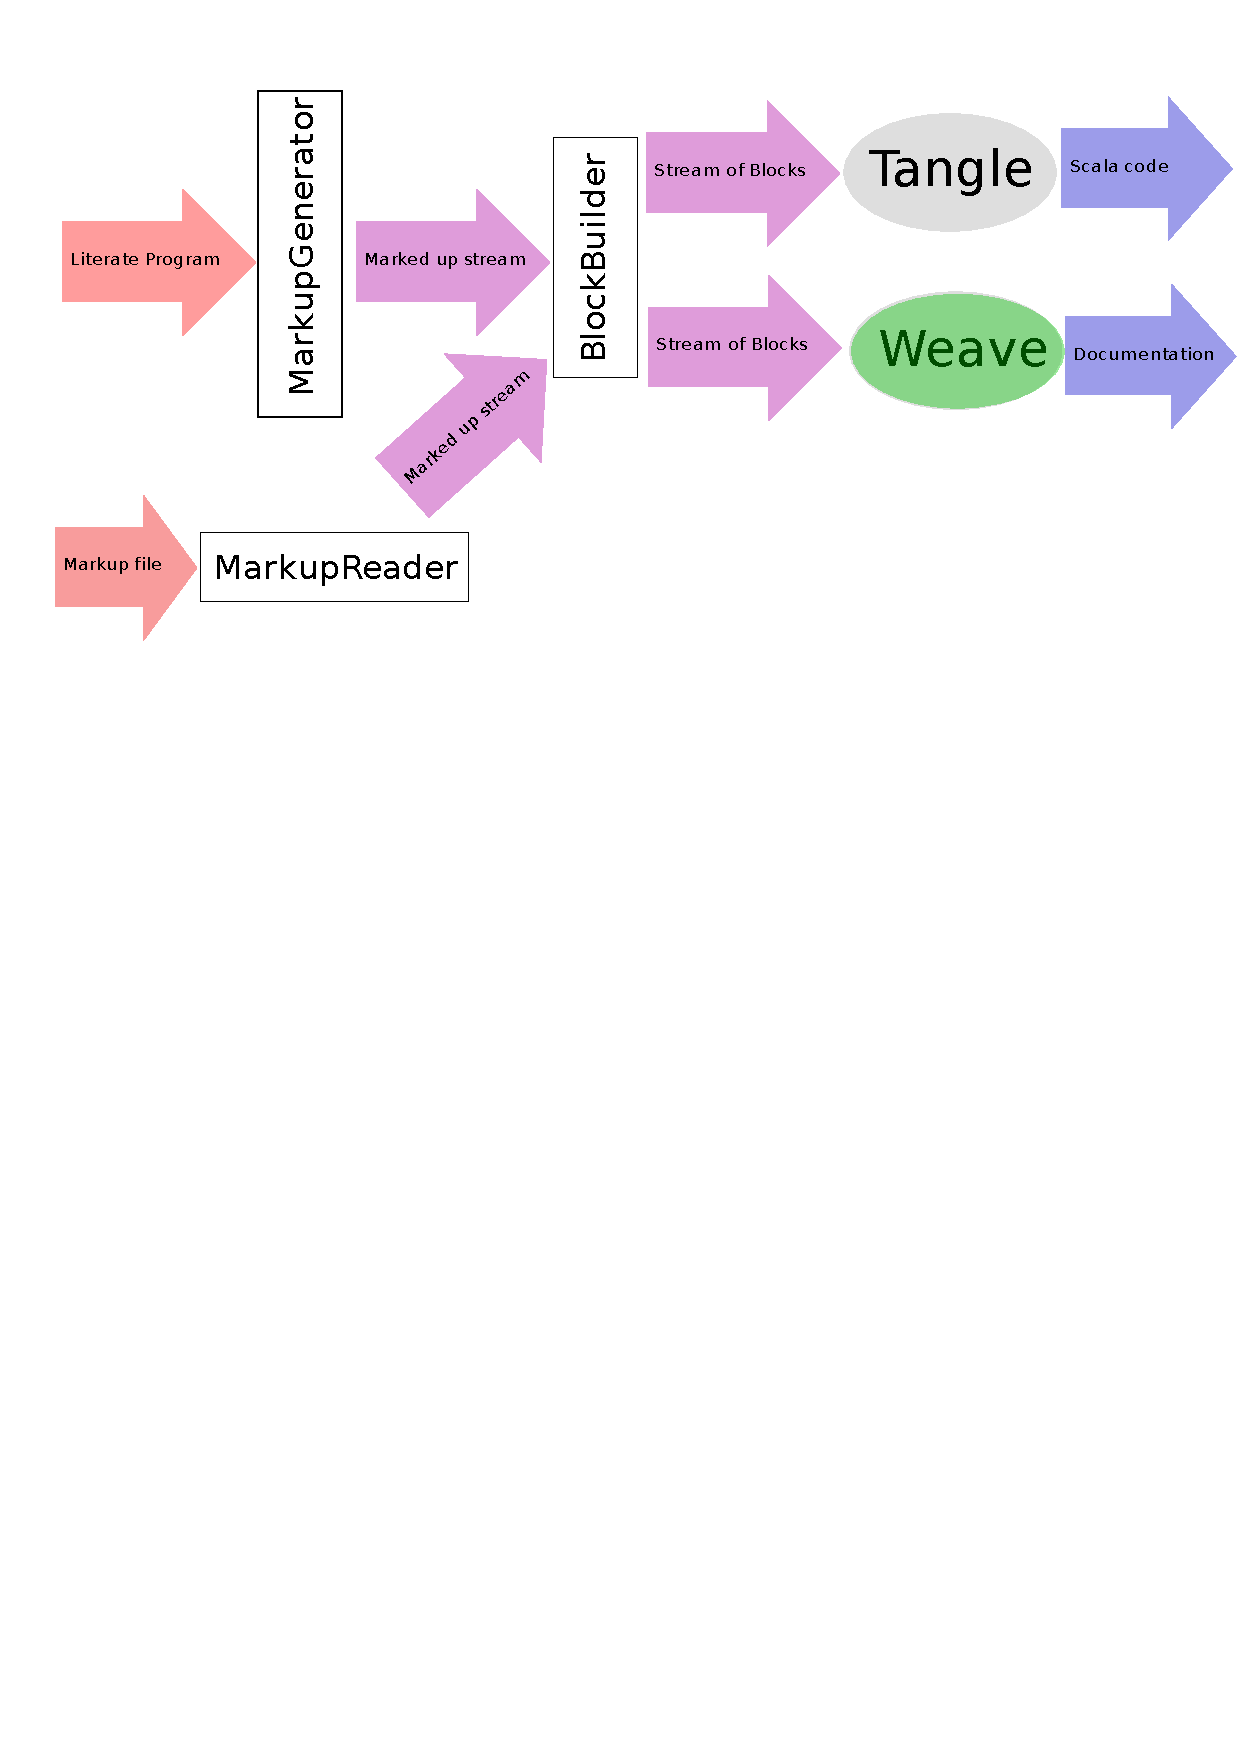
\includegraphics[width=10cm,viewport=310 610 600 710,clip]{images/weave}

It is important to note that there exists a tool to do syntactic
highlighting for scala called \texttt{verbfilter}\footnote{To be found under
misc/scala-tool-support/latex}. The method \texttt{process} takes a character
buffer and looks for \texttt{$\backslash$begin$\{$verbatim$\}$}, there it will begin to transform
the input. Our aim is therefore to convert the code sections to a character
buffer so that it can be fed to verbfilter.

$\left<\mbox{\emph{*}}\right>+\equiv$
\begin{program}{\vem package}~scalit.weave
\\{\vem import}~markup.\_
\\[0.5em]$<$The~LaTeX~weaver$>$
\\[0.5em]$<$Source~file~information$>$
\\[0.5em]$<$The~command~line~application$>$
\\[0.5em]\end{program}
\subsection{The LaTeX weaver}
LatexWeaver, the class that takes care of producing LaTeX output from a list of
streams of blocks (as defined in \texttt{weave/blocks.nw}) has two methods: One for
printing one block, \texttt{printBlock}, and one to print everything surrounding
to produce a valid LaTeX document.

$\left<\mbox{\emph{The LaTeX weaver}}\right>\equiv$
\begin{program}{\vem sealed}~{\vem abstract}~{\vem class}~Weaver$($blocks\,{\rm :}~List$[$$($Stream$[$Block$]$,String$)$$]$$)$
\\[0.5em]{\vem case}~{\vem class}~LatexWeaver$($blocks\,{\rm :}~List$[$$($Stream$[$Block$]$,String$)$$]$,
\\~~~~~~~~~~~~~~~~~~~~~~~~~~~~~~tangled\,{\rm :}~List$[$tangle.ChunkCollection$]$,
\\~~~~~~~~~~~~~~~~~~~~~~~~~~~~~~useVerbfilter\,{\rm :}~Boolean,
\\~~~~~~~~~~~~~~~~~~~~~~~~~~~~~~useIndex\,{\rm :}~Boolean,
\\~~~~~~~~~~~~~~~~~~~~~~~~~~~~~~classpath\,{\rm :}~Option$[$List$[$String$]$$]$,
\\~~~~~~~~~~~~~~~~~~~~~~~~~~~~~~filename\,{\rm :}~String,
\\~~~~~~~~~~~~~~~~~~~~~~~~~~~~~~useHeader\,{\rm :}~Boolean$)$
\\~~~~~~~~~~{\vem extends}~Weaver$($blocks$)$~{\small\{}
\\[0.5em]~~~~{\vem import}~java.io.PrintStream
\\[0.5em]~~~~$<$escape~in~quoted~sections$>$
\\[0.5em]~~~~$<$escape~code$>$
\\[0.5em]~~~~$<$print~one~block$>$
\\[0.5em]~~~~$<$print~the~document$>$
\\[0.5em]~~~~$<$compiler~help$>$
\\[0.5em]~~~~$<$format~index$>$
\\{\small\}}
\\[0.5em]\end{program}
The useVerbfilter flag tells the weaver whether it should fire up the compiler
to retreive information on the source code. This is made optional because
it is pretty expensive. If \texttt{useHeader} is set to false, then we will not
print a header (ideal for inclusion in other LaTeX files).

\subsection{Printing one block}
There are two types of blocks to consider, code and documentation blocks. In
documentation blocks, we will need to know how to escape content: The backslash
character especially has to be escaped.

$\left<\mbox{\emph{escape in quoted sections}}\right>\equiv$
\begin{program}~~~~{\vem def}~escape$($orig\,{\rm :}~String$)${\rm :}~String~=~{\small\{}
\\~~~~~~~~orig.replace$($"$\backslash$$\backslash$","\Dollar$\backslash$$\backslash$backslash\Dollar"$)$
\\~~~~~~~~~~~~~~~~.replace$($"{\small\{}","\Dollar$\backslash$$\backslash${\small\{}\Dollar"$)$
\\~~~~~~~~~~~~~~~~.replace$($"{\small\}}","\Dollar$\backslash$$\backslash${\small\}}\Dollar"$)$
\\~~~~~~~~~~~~~~~~.replace$($"\#","\Dollar$\backslash$$\backslash$\#\Dollar"$)$
\\~~~~~~~~~~~~~~~~.replace$($"$<$","\Dollar$\backslash$$\backslash$langle\Dollar"$)$
\\~~~~~~~~~~~~~~~~.replace$($"$>$","\Dollar$\backslash$$\backslash$rangle\Dollar"$)$
\\~~~~~~~~~~~~~~~~.replace$($"\_","$\backslash$$\backslash$\_"$)$
\\~~~~{\small\}}
\\[0.5em]\end{program}
This function will undoubtedly be extended by more escape sequences. Now on
how to actually print these blocks. One speciality that we want to indicate
is whether we have already begun the definition of a given chunk. As this
would be too cumbersome to carry around, we'll keep track of it here:

$\left<\mbox{\emph{print one block}}\right>\equiv$
\begin{program}~~~~{\vem val}~chunksSeen~=
\\~~~~~~~~{\vem new}~scala.collection.mutable.HashMap$[$String,CodeBlock$]$
\\[0.5em]\end{program}
On to the block printing:

$\left<\mbox{\emph{print one block}}\right>+\equiv$
\begin{program}~~~~{\vem import}~StringRefs.\_
\\~~~~{\vem def}~printBlock$($out\,{\rm :}~PrintStream,
\\~~~~~~~~~~~~~~~~~~chunks\,{\rm :}~tangle.ChunkCollection$)$
\\~~~~~~~~~~~~~~~~~~$($b\,{\rm :}~Block$)${\rm :}~Unit~=~b~{\vem match}~{\small\{}
\\~~~~~~~~{\vem case}~cb~@~CodeBlock$($bn,ln,content,blockname$)$~$\Rightarrow$~{\small\{}
\\~~~~~~~~~~~~out.print$($"\Dollar$\backslash$$\backslash$left$<$$\backslash$$\backslash$mbox{\small\{}$\backslash$$\backslash$emph{\small\{}"~$+$
\\~~~~~~~~~~~~~~~~~~~~blockname~$+$
\\~~~~~~~~~~~~~~~~~~~~"{\small\}}{\small\}}$\backslash$$\backslash$right$>$"$)$
\\[0.5em]~~~~~~~~~~~~{\vem if}$($~chunksSeen~contains~blockname~$)$~out.print$($"$+$"$)$
\\~~~~~~~~~~~~{\vem else}~chunksSeen~$+$=~$($blockname~$\rightarrow$~cb~$)$
\\[0.5em]~~~~~~~~~~~~out.println$($"$\backslash$$\backslash$equiv\Dollar"$)$
\\[0.5em]\end{program}
Chunks that get defined for the first time start with
$\left<name\right>\equiv$, a continued chunk will be of the
form $\left<name\right>+\equiv$. If we use other code chunks,
this will be noted by $\left<name\right>$. In the following
section we will slurp the whole content of the code block
into a string:

$\left<\mbox{\emph{print one block}}\right>+\equiv$
\begin{program}~~~~~~~~~~~~{\vem var}~begin~=~$-$1
\\~~~~~~~~~~~~{\vem var}~end~~~=~$-$1
\\~~~~~~~~~~~~{\vem val}~content~=~"$\backslash$$\backslash$begin{\small\{}verbatim{\small\}}"~$+$
\\~~~~~~~~~~~~$($$($cb.stringRefForm$($chunks.cm$)$~map~{\small\{}
\\~~~~~~~~~~~~~~~~{\vem case}~RealString$($cont,from,to$)$~$\Rightarrow$~{\small\{}
\\~~~~~~~~~~~~~~~~~~~~{\vem if}$($~begin~$==$~$-$1~$)$~begin~=~from
\\[0.5em]~~~~~~~~~~~~~~~~~~~~{\vem if}$($~to~$>$~end~$)$~end~=~to
\\[0.5em]~~~~~~~~~~~~~~~~~~~~cont
\\~~~~~~~~~~~~~~~~{\small\}}
\\~~~~~~~~~~~~~~~~{\vem case}~BlockRef$($b$)$~$\Rightarrow$~{\small\{}
\\~~~~~~~~~~~~~~~~~~~~"$<$"~$+$
\\~~~~~~~~~~~~~~~~~~~~b.blockname~$+$
\\~~~~~~~~~~~~~~~~~~~~"$>$"
\\~~~~~~~~~~~~~~~~{\small\}}
\\~~~~~~~~~~~~~~~~{\vem case}~other~$\Rightarrow$~error$($"Unexpected\,{\rm :}~"~$+$~other$)$
\\~~~~~~~~~~~~{\small\}}~foldLeft~""$)$~{\small\{}
\\~~~~~~~~~~~~~~~~$($acc\,{\rm :}~String,~next\,{\rm :}~String$)$~$\Rightarrow$~acc~$+$~next
\\~~~~~~~~~~~~{\small\}}$)$~$+$~"$\backslash$$\backslash$"~$+$~"end{\small\{}verbatim{\small\}}"
\\[0.5em]\end{program}
If we want to use verbfilter, then we'll pass it to the script.
As we will have some unescaping to do (especially the $\Dollar$
character is troublesome) the output is not directly sent to
out but stored in a byte array, on which we can then apply the
unescaping. Also, if we want to create an index, we'll have to tell
it here.

$\left<\mbox{\emph{print one block}}\right>+\equiv$
\begin{program}~~~~{\vem if}$($~useVerbfilter~$)$~{\small\{}
\\~~~~~~~~{\vem val}~vfOutput~=~{\vem new}~java.io.ByteArrayOutputStream
\\~~~~~~~~toolsupport.verbfilterScala
\\~~~~~~~~~~~~.process$($codeEscape$($content$)$.getBytes,vfOutput$)$
\\~~~~~~~~{\vem if}$($~useIndex~$)$
\\~~~~~~~~~~~~out.println$($
\\~~~~~~~~~~~~~~~~indexed$($
\\~~~~~~~~~~~~~~~~codeUnescape$($
\\~~~~~~~~~~~~~~~~vfOutput.toString$)$,
\\~~~~~~~~~~~~~~~~begin,end,chunks.filename$)$$)$
\\~~~~~~~~{\vem else}
\\~~~~~~~~~~~~out.println$($codeUnescape$($vfOutput.toString$)$$)$
\\~~~~{\small\}}~{\vem else}~{\small\{}
\\~~~~~~~~{\vem if}$($~useIndex~$)$
\\~~~~~~~~~~~~out.println$($indexed$($content,
\\~~~~~~~~~~~~~~~~begin,end,chunks.filename$)$$)$
\\~~~~~~~~{\vem else}
\\~~~~~~~~~~~~out.println$($content$)$
\\~~~~{\small\}}
\\{\small\}}
\\[0.5em]\end{program}
Here we just avoided a quine-like problem: \texttt{$\backslash$end$\{$verbatim$\}$} is the sequence
to terminate a code block, so if it occurs inside a code block, then we could
run into a problem.

Documentation blocks will contain escaped sections (quoted), but otherwise
they will be copied verbatim.

$\left<\mbox{\emph{print one block}}\right>+\equiv$
\begin{program}~~~~~~~~{\vem case}~d~@~DocuBlock$($bn,ln,content$)$~$\Rightarrow$~{\small\{}
\\~~~~~~~~~~~~d.stringRefForm$($Map$($$)$$)$~foreach~{\small\{}
\\~~~~~~~~~~~~~~~~x~$\Rightarrow$~x~{\vem match}~{\small\{}
\\~~~~~~~~~~~~~~~~~~~~{\vem case}~RealString$($cont,\_,\_$)$~$\Rightarrow$~out.print$($cont$)$
\\~~~~~~~~~~~~~~~~~~~~{\vem case}~QuotedString$($cont$)$~$\Rightarrow$~{\small\{}
\\~~~~~~~~~~~~~~~~~~~~~~~~out.print$($"$\backslash$$\backslash$texttt{\small\{}"$)$
\\~~~~~~~~~~~~~~~~~~~~~~~~out.print$($escape$($cont$)$$)$
\\~~~~~~~~~~~~~~~~~~~~~~~~out.print$($"{\small\}}"$)$
\\~~~~~~~~~~~~~~~~~~~~{\small\}}
\\~~~~~~~~~~~~~~~~~~~~{\vem case}~BlockRef$($\_$)$~$\Rightarrow$
\\~~~~~~~~~~~~~~~~~~~~~~~~error$($"Did~not~expect~code~reference"~$+$
\\~~~~~~~~~~~~~~~~~~~~~~~~"~in~documentation~chunk"$)$
\\~~~~~~~~~~~~~~~~{\small\}}
\\~~~~~~~~~~~~{\small\}}
\\~~~~~~~~{\small\}}
\\~~~~{\small\}}
\\[0.5em]\end{program}
\subsubsection{Escaping code}
As we will pass code to the \texttt{verbfilter} program afterwards, we have to 
be very careful with some code content that could also be interpreted as
LaTeX escape sequences: We have to strip them out:

$\left<\mbox{\emph{escape code}}\right>\equiv$
\begin{program}~~~~{\vem def}~codeEscape$($code\,{\rm :}~String$)${\rm :}~String~=~{\small\{}
\\~~~~~~~~code.replace$($"\Dollar","SPEC"~$+$~"DOLLAR"$)$
\\~~~~{\small\}}
\\[0.5em]\end{program}
The problem then is, of course, that we will need to put them back in
afterwards.

$\left<\mbox{\emph{escape code}}\right>+\equiv$
\begin{program}~~~~{\vem def}~codeUnescape$($code\,{\rm :}~String$)${\rm :}~String~=~{\small\{}
\\~~~~~~~~code.replace$($"SPEC"~$+$~"DOLLAR","$\backslash$$\backslash$Dollar"$)$
\\~~~~{\small\}}
\\[0.5em]\end{program}
\subsubsection{Wrapping the document}
With the knowledge on how to print blocks, we can go on printing the
whole document. If the useHeader flag is set (which it is by default),
we generate a standard LaTeX document, the only thing
special to note is that we add \texttt{scaladefs} which contains macros to
format scala output and \texttt{scalit} which enables definition indexing.

$\left<\mbox{\emph{print the document}}\right>\equiv$
\begin{program}~~~~{\vem def}~writeDoc$($out\,{\rm :}~PrintStream$)${\rm :}~Unit~=~{\small\{}
\\~~~~~~~~{\vem if}$($~useHeader~$)$~{\small\{}
\\~~~~~~~~~~~~out.println$($"$\backslash$$\backslash$documentclass$[$a4paper,12pt$]${\small\{}article{\small\}}"$)$
\\~~~~~~~~~~~~out.println$($"$\backslash$$\backslash$usepackage{\small\{}amsmath,amssymb{\small\}}"$)$
\\~~~~~~~~~~~~out.println$($"$\backslash$$\backslash$usepackage{\small\{}graphicx{\small\}}"$)$
\\~~~~~~~~~~~~out.println$($"$\backslash$$\backslash$usepackage{\small\{}scaladefs{\small\}}"$)$
\\~~~~~~~~~~~~out.println$($"$\backslash$$\backslash$usepackage{\small\{}scalit{\small\}}"$)$
\\~~~~~~~~~~~~out.println$($"$\backslash$$\backslash$usepackage{\small\{}fancyhdr{\small\}}"$)$
\\~~~~~~~~~~~~out.println$($"$\backslash$$\backslash$pagestyle{\small\{}fancy{\small\}}"$)$
\\~~~~~~~~~~~~out.println$($"$\backslash$$\backslash$lhead{\small\{}$\backslash$$\backslash$today{\small\}}"$)$
\\~~~~~~~~~~~~out.println$($"$\backslash$$\backslash$rhead{\small\{}"~$+$~escape$($filename$)$~$+$~"{\small\}}"$)$
\\~~~~~~~~~~~~out.println$($"$\backslash$$\backslash$begin{\small\{}document{\small\}}"$)$
\\~~~~~~~~{\small\}}
\\~~~~~~~~
\\~~~~~~~~blocks~zip~tangled~foreach~{\small\{}
\\~~~~~~~~~~~~{\vem case}~$($$($bs,\_$)$,tang$)$~$\Rightarrow$~bs~foreach~printBlock$($out,tang$)$
\\~~~~~~~~{\small\}}
\\[0.5em]~~~~~~~~{\vem if}$($~useHeader~$)$~{\small\{}
\\~~~~~~~~~~~~out.println$($"$\backslash$$\backslash$end{\small\{}document{\small\}}$\backslash$n$\backslash$n"$)$
\\~~~~~~~~{\small\}}
\\~~~~{\small\}}
\\[0.5em]\end{program}
\subsection{Information on the source file}
During tangling, we directly interact with the compiler to compile from literate
programs. But the compiler can be of much more help - We can for example find
out where classes are defined, etc. For this, we reuse the source file class
defined for literate compilation\footnote{tangle/compilesupport.nw}.

Another optional parameter is where to find the classes containing
the other definitions: This will be used by the compiler to typecheck
the code, thus generating the symbols we need.

$\left<\mbox{\emph{Source file information}}\right>\equiv$
\begin{program}{\vem import}~scala.tools.nsc.ast.Trees
\\{\vem class}~SourceInformation$($
\\~~~~literateFile\,{\rm :}~tangle.LiterateProgramSourceFile,
\\~~~~infoClassPath\,{\rm :}~Option$[$List$[$String$]$$]$$)$~{\small\{}
\\~~~~$<$Instantiate~a~compiler$>$
\\[0.5em]~~~~$<$collect~information$>$
\\~~~~$<$range~of~definitions$>$
\\{\small\}}
\\[0.5em]$<$Definition~info~storage$>$
\\[0.5em]\end{program}
as with the compiler support class, we'll have to instantiate
a compiler. However, we will not need to do all the phases,
so we overwrite the phases we need:

$\left<\mbox{\emph{Instantiate a compiler}}\right>\equiv$
\begin{program}~~~~{\vem import}~scala.tools.nsc.{\small\{}Global,Settings,SubComponent{\small\}}
\\~~~~{\vem import}~scala.tools.nsc.reporters.ConsoleReporter
\\[0.5em]~~~~{\vem val}~settings~=~{\vem new}~Settings$($$)$
\\~~~~infoClassPath~{\vem match}~{\small\{}
\\~~~~~~~~{\vem case}~None~$\Rightarrow$~$($$)$
\\~~~~~~~~{\vem case}~Some$($cp$)$~$\Rightarrow$~settings.classpath.value~=~cp.head
\\~~~~{\small\}}
\\[0.5em]~~~~{\vem val}~reporter~=
\\~~~~~~~~{\vem new}~ConsoleReporter$($settings,{\vem null},
\\~~~~~~~~~~~~~~~~~~~~~~~~~~~~~~~~~~~~~~~~~~~~~~~~{\vem new}~java.io.PrintWriter$($System.err$)$$)$
\\~~~~{\vem object}~compiler~{\vem extends}~Global$($settings,~reporter$)$~{\small\{}
\\~~~~~~~~{\vem override}~{\vem protected}~{\vem def}~builtInPhaseDescriptors\,{\rm :}
\\~~~~~~~~List$[$SubComponent$]$~=~List$($
\\~~~~~~~~~~~~analyzer.namerFactory\,{\rm :}~SubComponent,
\\~~~~~~~~~~~~analyzer.typerFactory\,{\rm :}~SubComponent
\\~~~~~~~~$)$
\\~~~~{\small\}}
\\[0.5em]\end{program}
with the compiler in place, we can now define how to collect the information:

Execute the compiler just up to typing and collect them from the syntax tree.

$\left<\mbox{\emph{collect information}}\right>\equiv$
\begin{program}~~~~{\vem lazy}~{\vem val}~info~=~{\small\{}
\\~~~~~~~~{\vem val}~r~=~{\vem new}~compiler.Run
\\~~~~~~~~r.compileSources$($literateFile~{\rm :}{\rm :}~Nil$)$
\\[0.5em]~~~~~~~~{\vem val}~typedUnit~=~r.units.next
\\[0.5em]~~~~~~~~collectDefinitions$($typedUnit.body,Map$($$)$$)$
\\~~~~{\small\}}
\\[0.5em]\end{program}
The definition collector needs to have access to the tree case classes. They
are part of the compiler. We are very forgiving if, for example we do not find
a valid position.

$\left<\mbox{\emph{collect information}}\right>+\equiv$
\begin{program}~~~~{\vem import}~compiler.{\small\{}Tree,ClassDef,ModuleDef,PackageDef,
\\~~~~~~~~~~~~~~~~~~~~~~~~~~~~~~~~~~~~~~DefDef,ValDef,Template{\small\}}
\\~~~~{\vem import}~DefinitionInfo.\_
\\[0.5em]\end{program}
We will want to have access to the information on a per-line-basis. However,
there will be multiple definitions on one line, so we will need something like
a multiset:

$\left<\mbox{\emph{collect information}}\right>+\equiv$
\begin{program}~~~~{\vem type}~DefMap~=~Map$[$Int,Set$[$Definition$]$$]$
\\[0.5em]\end{program}
Another useful state to store is in which class we currently are, so that
we can link methods (which might be defined in multiple classes) to a specific
class. We overload this method to stay succinct.

$\left<\mbox{\emph{collect information}}\right>+\equiv$
\begin{program}~~~~{\vem def}~collectDefinitions$($t\,{\rm :}~Tree,~acc\,{\rm :}~DefMap$)${\rm :}~DefMap~=
\\~~~~~~~~collectDefinitions$($t,acc,None$)$
\\[0.5em]~~~~{\vem def}~collectDefinitions$($t\,{\rm :}~Tree,
\\~~~~~~~~~~~~~~~~~~~~~~~~~~~~~~~~~~acc\,{\rm :}~DefMap,
\\~~~~~~~~~~~~~~~~~~~~~~~~~~~~~~~~~~container\,{\rm :}~Option$[$String$]$$)${\rm :}~DefMap~=~{\small\{}
\\[0.5em]\end{program}
After these overloaded definitions, let'l begin by getting the
source file position:

$\left<\mbox{\emph{collect information}}\right>+\equiv$
\begin{program}~~~~~~~~{\vem val}~pos~=~literateFile.positionInUltimateSource$($t.pos$)$
\\~~~~~~~~{\vem val}~line~=~pos.line~{\vem match}~{\small\{}
\\~~~~~~~~~~~~{\vem case}~None~$\Rightarrow$~$-$1
\\~~~~~~~~~~~~{\vem case}~Some$($l$)$~$\Rightarrow$~l
\\~~~~~~~~{\small\}}
\\~~~~~~~~{\vem val}~before~=~acc.getOrElse$($line,Set$($$)$$)$
\\~~~~~~~~t~{\vem match}~{\small\{}
\\$<$Handle~the~{\vem class}~{\vem case}$>$
\\$<$Handle~the~{\vem object}~{\vem case}$>$
\\$<$Handle~the~{\vem package}~{\vem case}$>$
\\$<$Handle~the~method~{\vem case}$>$
\\$<$Handle~the~value~{\vem case}$>$
\\~~~~~~~~~~~~{\vem case}~other~$\Rightarrow$~acc
\\~~~~~~~~{\small\}}
\\~~~~{\small\}}
\\[0.5em]\end{program}
The accumulator style makes this function rather heavy (note all the folds),
but this way we can append the definitions in a predictable style. So, on to the
starting point in our tree: The package definition

$\left<\mbox{\emph{Handle the package case}}\right>\equiv$
\begin{program}~~~~~~~~~~~~{\vem case}~PackageDef$($name,stats$)$~$\Rightarrow$
\\~~~~~~~~~~~~~~~~$($stats~foldLeft~acc$)$~{\small\{}
\\~~~~~~~~~~~~~~~~~~~~$($defs\,{\rm :}~DefMap,~t\,{\rm :}~Tree$)$~$\Rightarrow$~collectDefinitions$($t,defs$)$
\\~~~~~~~~~~~~~~~~{\small\}}
\\[0.5em]\end{program}
\texttt{defs} holds the current state of the map. Nodes of this package definition
will be classes and objects. We will first collect everything in the first class,
then pass the definition results to the second class, etc. Here is what we do with
classes:

$\left<\mbox{\emph{Handle the class case}}\right>\equiv$
\begin{program}{\vem case}~ClassDef$($\_,name,tparams,impl$)$~$\Rightarrow$
\\~~~~{\vem val}~nameString~=~name.toChars~mkString~""
\\~~~~{\vem val}~newAcc~=
\\~~~~~~~~acc~$+$~$($line~$\rightarrow$~$($before~$+$
\\~~~~~~~~~~~~~~~~~~~~~~~~~~~~~~~~~~~~~~~~ClassDefinition$($nameString,line,{\vem false}$)$$)$$)$
\\~~~~impl~{\vem match}~{\small\{}
\\~~~~~~~~{\vem case}~Template$($\_,\_,body$)$~$\Rightarrow$
\\~~~~~~~~~~~~$($body~foldLeft~newAcc$)$~{\small\{}
\\~~~~~~~~~~~~~~~~$($defs\,{\rm :}~DefMap,~t\,{\rm :}~Tree$)$~$\Rightarrow$
\\~~~~~~~~~~~~~~~~~~~~collectDefinitions$($t,defs,Some$($nameString$)$$)$
\\~~~~~~~~~~~~{\small\}}
\\~~~~{\small\}}
\\[0.5em]\end{program}
Classes have a body which we need to scan, but before we will have to add the class
itself to the map. If only that were so easy! Note that there are three basic types
of top-level objects on the class level:

\begin{itemize}
\item ``Normal'' classes
\item Objects
\item Case classes / objects
\end{itemize}

Note that this is not an either/or decision. A normal way to emulate static members in
Scala is the following:

\begin{verbatim}
class A {
  def aMethod = A.staticOne()
}
object A {
  def staticOne() = ...
}
\end{verbatim}

So we will be allowed to have object definitions and class definitions on different
lines. The compiler, however, seems to generate both \texttt{ClassDef} and \texttt{ModuleDef}
nodes when we have a case class. Also, the definition map is in an incomplete state,
so we can only bet on not seeing another \texttt{ClassDef} afterwards by assuming what
the compiler generates first the module definition element.
This first test tells us to only add contents if we are sure this actually is an
object. If we are dealing with a case class, we'll have to indicate this, for this
we will use the variable classDefinition.

$\left<\mbox{\emph{Do not add if object is there}}\right>\equiv$
\begin{program}~~~~~~~~~~~~~~~~{\vem var}~classDefinition\,{\rm :}~Option$[$ClassDefinition$]$~=~None
\\~~~~~~~~~~~~~~~~{\vem val}~isRealObject~=~acc~get~line~{\vem match}~{\small\{}
\\~~~~~~~~~~~~~~~~~~~~{\vem case}~Some$($s$)$~$\Rightarrow$~!$($s~exists~{\small\{}
\\~~~~~~~~~~~~~~~~~~~~~~~~{\vem case}~cd~@~ClassDefinition$($n,\_,\_$)$~$\Rightarrow$~{\small\{}
\\~~~~~~~~~~~~~~~~~~~~~~~~~~~~{\vem if}$($~n~$==$~nameString~$)$~{\small\{}
\\~~~~~~~~~~~~~~~~~~~~~~~~~~~~~~~~classDefinition~=~Some$($cd$)$
\\~~~~~~~~~~~~~~~~~~~~~~~~~~~~~~~~{\vem true}
\\~~~~~~~~~~~~~~~~~~~~~~~~~~~~{\small\}}~{\vem else}~{\vem false}
\\~~~~~~~~~~~~~~~~~~~~~~~~{\small\}}
\\~~~~~~~~~~~~~~~~~~~~~~~~{\vem case}~other~$\Rightarrow$~{\vem false}
\\~~~~~~~~~~~~~~~~~~~~{\small\}}$)$
\\~~~~~~~~~~~~~~~~~~~~{\vem case}~None~$\Rightarrow$~~~~~~~~~{\vem true}
\\~~~~~~~~~~~~~~~~{\small\}}
\\[0.5em]\end{program}
If we have already content on this line, then we will not traverse it again, but
we will update the fact that we are dealing with a case class.

$\left<\mbox{\emph{Handle the object case}}\right>\equiv$
\begin{program}{\vem case}~ModuleDef$($mods,name,impl$)$~$\Rightarrow$
\\~~~~{\vem val}~nameString~=~name.toChars~mkString~""
\\~~~~$<$Do~not~add~{\vem if}~{\vem object}~is~there$>$
\\~~~~{\vem if}$($isRealObject$)$~{\small\{}
\\~~~~~~~~{\vem val}~newAcc~=~acc~$+$~$($line~$\rightarrow$
\\~~~~~~~~~~~~~~~~$($before~$+$~ObjectDefinition$($nameString,line$)$$)$$)$
\\~~~~~~~~impl~{\vem match}~{\small\{}
\\~~~~~~~~~~~~{\vem case}~Template$($\_,\_,body$)$~$\Rightarrow$
\\~~~~~~~~~~~~~~~~$($body~foldLeft~newAcc$)$~{\small\{}
\\~~~~~~~~~~~~~~~~~~~~$($defs\,{\rm :}~DefMap,~t\,{\rm :}~Tree$)$~$\Rightarrow$
\\~~~~~~~~~~~~~~~~~~~~~~~~collectDefinitions$($t,defs,Some$($nameString$)$$)$
\\~~~~~~~~~~~~~~~~{\small\}}
\\~~~~~~~~{\small\}}
\\~~~~{\small\}}~{\vem else}~{\small\{}
\\~~~~~~~~{\vem val}~Some$($cd$)$~=~classDefinition
\\~~~~~~~~{\vem val}~cc~=~ClassDefinition$($cd.name,cd.l,{\vem true}$)$
\\~~~~~~~~acc~$+$~$($line~$\rightarrow$~$($before~$-$~cd~$+$~cc$)$$)$
\\~~~~{\small\}}
\\[0.5em]\end{program}
For the definitions, We will have to use the same trick as for objects: Some
methods are added automatically (like toString, <init>) and should therefore not
be included in the index. We solve this by looking up whether a class was defined
on the same line. Also, it might be that there exists already a value definition with
the same name, in which case we won't add it either:

$\left<\mbox{\emph{Handle the method case}}\right>\equiv$
\begin{program}{\vem case}~DefDef$($\_,name,tparams,vparams,tpt,\_$)$~$\Rightarrow$
\\~~~~{\vem val}~isGeneratedMethod~=~acc~get~line~{\vem match}~{\small\{}
\\~~~~~~~~{\vem case}~None~$\Rightarrow$~{\vem false}
\\~~~~~~~~{\vem case}~Some$($s$)$~$\Rightarrow$~s~exists~{\small\{}
\\~~~~~~~~~~~~{\vem case}~c~{\rm :}~ClassDefinition~$\Rightarrow$~{\vem true}
\\~~~~~~~~~~~~{\vem case}~o~{\rm :}~ObjectDefinition~$\Rightarrow$~{\vem true}
\\~~~~~~~~~~~~{\vem case}~vd~{\rm :}~ValueDefinition~$\Rightarrow$~{\vem true}
\\~~~~~~~~~~~~{\vem case}~\_~$\Rightarrow$~{\vem false}
\\~~~~~~~~{\small\}}
\\~~~~{\small\}}
\\~~~~{\vem if}$($~isGeneratedMethod~$)$~acc
\\~~~~{\vem else}~acc~$+$~$($line~$\rightarrow$
\\~~~~~~~~$($before~$+$~MethodDefinition$($name.toString,line,container$)$$)$$)$
\\[0.5em]\end{program}
We also record value definitions

$\left<\mbox{\emph{Handle the value case}}\right>\equiv$
\begin{program}~~~~~~~~~~~~{\vem case}~ValDef$($\_,name,\_,\_$)$~$\Rightarrow$~{\small\{}
\\~~~~~~~~~~~~~~~~{\vem val}~nameString~=~name.toChars~mkString~""
\\~~~~~~~~~~~~~~~~acc~$+$~$($line~$\rightarrow$~$($before~$+$~ValueDefinition$($nameString,line,container$)$$)$$)$~
\\~~~~~~~~~~~~{\small\}}
\\[0.5em]\end{program}
 One useful
command would be to get all the definitions in a range of lines:

$\left<\mbox{\emph{range of definitions}}\right>\equiv$
\begin{program}~~~~{\vem def}~getRange$($from\,{\rm :}~Int,~to\,{\rm :}~Int$)${\rm :}~List$[$Definition$]$~=
\\~~~~~~~~List.range$($from,to~$+$~1$)$~flatMap~{\small\{}
\\~~~~~~~~~~~~i~$\Rightarrow$~info.getOrElse$($i,Nil$)$
\\~~~~~~~~{\small\}}
\\[0.5em]\end{program}
\subsubsection{Connection to the weaver}
Especially in LaTeXWeaver, we will want to auto-generate some annotations,
therefore we'll have to have a value for that:

$\left<\mbox{\emph{compiler help}}\right>\equiv$
\begin{program}~~~~{\vem import}~tangle.LiterateProgramSourceFile
\\~~~~{\vem val}~sourcefiles\,{\rm :}~Option$[$List$[$$($String,LiterateProgramSourceFile$)$$]$$]$~=
\\~~~~~~~~{\vem if}$($~useIndex~$)$~{\small\{}
\\~~~~~~~~~~~~Some$($tangled~map~{\small\{}
\\~~~~~~~~~~~~~~~~chunks~$\Rightarrow$
\\~~~~~~~~~~~~~~~~~~~~$($chunks.filename,
\\~~~~~~~~~~~~~~~~~~~~~~{\vem new}~tangle.LiterateProgramSourceFile$($chunks$)$$)$
\\~~~~~~~~~~~~{\small\}}$)$
\\~~~~~~~~{\small\}}~{\vem else}~None
\\[0.5em]~~~~{\vem val}~sourceInformation\,{\rm :}~Map$[$String,SourceInformation$]$~=
\\~~~~sourcefiles~{\vem match}~{\small\{}
\\~~~~~~~~{\vem case}~None~$\Rightarrow$~Map$($$)$
\\~~~~~~~~{\vem case}~Some$($sfs$)$~$\Rightarrow$~Map$($$)$~$+$$+$~$($sfs~map~{\small\{}
\\~~~~~~~~~~~~{\vem case}~$($name,sf$)$~$\Rightarrow$~$($name~$\rightarrow$~{\vem new}~SourceInformation$($sf,classpath$)$$)$
\\~~~~~~~~{\small\}}$)$
\\~~~~{\small\}}
\\[0.5em]\end{program}
\subsubsection{Storing the gathered information}
While traversing the tree, we need to store information on what is actually
defined. This is particularly:

\begin{itemize}
\item Class and trait definitions
\item Object definitions
\item Method definitions
\end{itemize}

To each element, we'll want to store the line number so that it can be easily
retrieved.

$\left<\mbox{\emph{Definition info storage}}\right>\equiv$
\begin{program}{\vem object}~DefinitionInfo~{\small\{}
\\~~~~{\vem sealed}~{\vem abstract}~{\vem class}~Definition$($line\,{\rm :}~Int$)$
\\[0.5em]~~~~{\vem case}~{\vem class}~ClassDefinition$($name\,{\rm :}~String,~l\,{\rm :}~Int,
\\~~~~~~~~~~~~~~~~~~~~~~~~~~~~~~~~~~~~~~~~~~~~~~~~~~isCase\,{\rm :}~Boolean$)$
\\~~~~~~~~{\vem extends}~Definition$($l$)$~{\small\{}
\\~~~~~~~~~~~~{\vem override}~{\vem def}~toString~=~""~$+$~l~$+$~"{\rm :}~Class~"~$+$~name
\\~~~~~~~~{\small\}}
\\[0.5em]~~~~{\vem case}~{\vem class}~ObjectDefinition$($name\,{\rm :}~String,
\\~~~~~~~~~~~~~~~~~~~~~~~~~~~~~~~~~~~~~~~~~~~~~~~~~~l\,{\rm :}~Int$)$
\\~~~~~~~~{\vem extends}~Definition$($l$)$~{\small\{}
\\~~~~~~~~~~~~{\vem override}~{\vem def}~toString~=~""~$+$~l~$+$~"{\rm :}~Object~"~$+$~name
\\~~~~~~~~{\small\}}
\\[0.5em]~~~~{\vem case}~{\vem class}~MethodDefinition$($name\,{\rm :}~String,
\\~~~~~~~~~~~~~~~~~~~~~~~~~~~~~~~~~~~~~~~~~~~~~~~~~~l\,{\rm :}~Int,
\\~~~~~~~~~~~~~~~~~~~~~~~~~~~~~~~~~~~~~~~~~~~~~~~~~~container\,{\rm :}~Option$[$String$]$$)$
\\~~~~~~~~{\vem extends}~Definition$($l$)$~{\small\{}
\\~~~~~~~~~~~~{\vem override}~{\vem def}~toString~=~""~$+$~l~$+$~"{\rm :}~Method~"~$+$~name
\\~~~~~~~~{\small\}}
\\[0.5em]~~~~{\vem case}~{\vem class}~ValueDefinition$($name\,{\rm :}~String,
\\~~~~~~~~~~~~~~~~~~~~~~~~~~~~~~~~~~~~~~~~~~~~~~~~~~l\,{\rm :}~Int,
\\~~~~~~~~~~~~~~~~~~~~~~~~~~~~~~~~~~~~~~~~~~~~~~~~~~container\,{\rm :}~Option$[$String$]$$)$
\\~~~~~~~~{\vem extends}~Definition$($l$)$~{\small\{}
\\~~~~~~~~~~~~{\vem override}~{\vem def}~toString~=~""~$+$~l~$+$~"{\rm :}~Value~"~$+$~name
\\~~~~~~~~{\small\}}
\\{\small\}}
\\[0.5em]\end{program}
\subsubsection{Testing the information gathering}
The following command line tool tests the information gathering:

$\left<\mbox{\emph{Source file information}}\right>+\equiv$
\begin{program}{\vem object}~InfoTester~{\small\{}
\\~~~~{\vem def}~main$($args\,{\rm :}~Array$[$String$]$$)$~=~{\small\{}
\\~~~~~~~~{\vem import}~util.LiterateSettings
\\~~~~~~~~{\vem import}~tangle.LiterateProgramSourceFile
\\[0.5em]
\\~~~~~~~~{\vem val}~ls~=~{\vem new}~LiterateSettings$($args$)$
\\[0.5em]~~~~~~~~{\vem val}~sourceFiles~=
\\~~~~~~~~~~~~ls.chunkCollections~map~$($
\\~~~~~~~~~~~~~~~~{\vem new}~LiterateProgramSourceFile$($\_$)$$)$
\\[0.5em]~~~~~~~~{\vem val}~infoclasspath~=~ls.settings~get~"$-$classpath"
\\[0.5em]~~~~~~~~{\vem val}~infolist~=
\\~~~~~~~~~~~~sourceFiles~map~$(${\vem new}~SourceInformation$($\_,infoclasspath$)$$)$
\\[0.5em]~~~~~~~~infolist~foreach~{\small\{}~x~$\Rightarrow$~println$($x.getRange$($0,50$)$$)$~{\small\}}
\\~~~~{\small\}}
\\{\small\}}
\\[0.5em]\end{program}
\subsubsection{Adding index information}
With the compiler support that we defined before, we will be able to print
which functions were defined in a piece of code. The following function adds
these bits:

$\left<\mbox{\emph{format index}}\right>\equiv$
\begin{program}~~~~{\vem def}~indexed$($content\,{\rm :}~String,~from\,{\rm :}~Int,
\\~~~~~~~~~~~~~~~~~~~~~~~~~~~~to\,{\rm :}~Int,~filename\,{\rm :}~String$)${\rm :}~String~=~{\small\{}
\\~~~~~~~~{\vem import}~DefinitionInfo.\_
\\~~~~~~~~{\vem val}~ret~=~{\vem new}~StringBuffer
\\~~~~~~~~ret~append~content
\\~~~~~~~~
\\~~~~~~~~sourceInformation~get~filename~{\vem match}~{\small\{}
\\~~~~~~~~~~~~{\vem case}~None~$\Rightarrow$~$($$)$
\\~~~~~~~~~~~~{\vem case}~Some$($si$)$~$\Rightarrow$~{\small\{}
\\~~~~~~~~~~~~~~~~{\vem val}~definitions~=~si.getRange$($from,to$)$
\\[0.5em]\end{program}
The first definitions that we are interested in are which classes
are defined:

$\left<\mbox{\emph{format index}}\right>+\equiv$
\begin{program}~~~~~~~~~~~~~~~~{\vem val}~classes~=~definitions~filter~{\small\{}
\\~~~~~~~~~~~~~~~~~~~~{\vem case}~cd\,{\rm :}~ClassDefinition~$\Rightarrow$~{\vem true}
\\~~~~~~~~~~~~~~~~~~~~{\vem case}~\_~$\Rightarrow$~{\vem false}
\\~~~~~~~~~~~~~~~~{\small\}}
\\[0.5em]\end{program}
Then methods. Here, we want to filter out the generated methods

$\left<\mbox{\emph{format index}}\right>+\equiv$
\begin{program}~~~~~~~~~~~~~~~~{\vem val}~methods~=~definitions~filter~{\small\{}
\\~~~~~~~~~~~~~~~~~~~~{\vem case}~MethodDefinition$($name,\_,\_$)$~$\Rightarrow$~{\vem true}
\\~~~~~~~~~~~~~~~~~~~~{\vem case}~\_~$\Rightarrow$~{\vem false}
\\~~~~~~~~~~~~~~~~{\small\}}
\\[0.5em]\end{program}
Values and objects are filtered in a same way

$\left<\mbox{\emph{format index}}\right>+\equiv$
\begin{program}~~~~~~~~~~~~~~~~{\vem val}~values~=~definitions~filter~{\small\{}
\\~~~~~~~~~~~~~~~~~~~~{\vem case}~v~{\rm :}~ValueDefinition~$\Rightarrow$~{\vem true}
\\~~~~~~~~~~~~~~~~~~~~{\vem case}~\_~$\Rightarrow$~{\vem false}
\\~~~~~~~~~~~~~~~~{\small\}}
\\~~~~~~~~~~~~~~~~{\vem val}~objects~=~definitions~filter~{\small\{}
\\~~~~~~~~~~~~~~~~~~~~{\vem case}~o\,{\rm :}~ObjectDefinition~$\Rightarrow$~{\vem true}
\\~~~~~~~~~~~~~~~~~~~~{\vem case}~\_~$\Rightarrow$~{\vem false}
\\~~~~~~~~~~~~~~~~{\small\}}
\\[0.5em]\end{program}
Now for the LaTeX output generated: We use the commands defined
in \texttt{scalit.sty} so that we can change presentation later on. Note that
no real output needs to be generated.

$\left<\mbox{\emph{format index}}\right>+\equiv$
\begin{program}~~~~~~~~~~~~~~~~{\vem if}~$($!classes.isEmpty~$\,|$$\,|$~!methods.isEmpty~$\,|$$\,|$
\\~~~~~~~~~~~~~~~~~~~~~~~~!objects.isEmpty$)$~{\small\{}
\\$<$output~{\vem class}~definition~info$>$
\\$<$output~{\vem object}~definition~info$>$
\\$<$output~method~definition~info$>$
\\$<$output~value~definition~info$>$
\\~~~~~~~~~~~~~~~~{\small\}}
\\~~~~~~~~~~~~~~~~ret~append~"$\backslash$n$\backslash$n"
\\~~~~~~~~~~~~{\small\}}
\\~~~~~~~~{\small\}}
\\[0.5em]~~~~~~~~ret.toString
\\~~~~{\small\}}
\\[0.5em]\end{program}
First the classes. The command \texttt{classdefinition} takes care
of them. At the moment, we are not indicating case classes specially.

$\left<\mbox{\emph{output class definition info}}\right>\equiv$
\begin{program}classes~foreach~{\small\{}
\\~~~~{\vem case}~ClassDefinition$($name,\_,caseClass$)$~$\Rightarrow$~{\small\{}
\\~~~~~~~~ret~append~"$\backslash$$\backslash$classdefinition{\small\{}"~$+$~name~$+$~"{\small\}}$\backslash$n"
\\~~~~{\small\}}
\\~~~~{\vem case}~\_~$\Rightarrow$~$($$)$
\\{\small\}}
\\[0.5em]\end{program}
Second come the object definitions.

$\left<\mbox{\emph{output object definition info}}\right>\equiv$
\begin{program}objects~foreach~{\small\{}
\\~~~~{\vem case}~ObjectDefinition$($name,\_$)$~$\Rightarrow$~{\small\{}
\\~~~~~~~~ret~append~"$\backslash$$\backslash$objectdefinition{\small\{}"~$+$~name~$+$~"{\small\}}$\backslash$n"
\\~~~~{\small\}}
\\~~~~{\vem case}~\_~$\Rightarrow$~$($$)$
\\{\small\}}
\\[0.5em]\end{program}
Methods are prefixed by the class in which they are defined. Note
the flaw in this system: This way we are only recording one level
of classes, thus generating a flat index. Also, the body of the
methods is not further traversed, so inner functions are not
detected.

$\left<\mbox{\emph{output method definition info}}\right>\equiv$
\begin{program}methods~foreach~{\small\{}
\\~~~~{\vem case}~MethodDefinition$($name,\_,cont$)$~$\Rightarrow$~{\small\{}
\\~~~~~~~~ret~append~"$\backslash$$\backslash$methoddefinition{\small\{}"
\\~~~~~~~~cont~{\vem match}~{\small\{}
\\~~~~~~~~~~~~{\vem case}~None~$\Rightarrow$~$($$)$
\\~~~~~~~~~~~~~~~~{\vem case}~Some$($n$)$~$\Rightarrow$~ret~append~escape$($n$)$
\\~~~~~~~~{\small\}}
\\~~~~~~~~ret~append~"{\small\}}{\small\{}"
\\~~~~~~~~ret~append~escape$($name$)$~$+$~"{\small\}}$\backslash$n"
\\~~~~{\small\}}
\\~~~~{\vem case}~\_~$\Rightarrow$~$($$)$
\\{\small\}}
\\[0.5em]\end{program}
Value definitions are also noted. This might be a bit
overkill, so in a further stage we could filter for only
publicly accessible values.

$\left<\mbox{\emph{output value definition info}}\right>\equiv$
\begin{program}values~foreach~{\small\{}
\\~~~~{\vem case}~ValueDefinition$($name,\_,cont$)$~$\Rightarrow$~{\small\{}
\\~~~~~~~~ret~append~"$\backslash$$\backslash$valuedefinition{\small\{}"
\\~~~~~~~~cont~{\vem match}~{\small\{}
\\~~~~~~~~~~~~{\vem case}~None~$\Rightarrow$~$($$)$
\\~~~~~~~~~~~~~~~~{\vem case}~Some$($n$)$~$\Rightarrow$~ret~append~escape$($n$)$
\\~~~~~~~~{\small\}}
\\~~~~~~~~ret~append~"{\small\}}{\small\{}"
\\~~~~~~~~ret~append~name~$+$~"{\small\}}$\backslash$n"
\\~~~~{\small\}}
\\~~~~{\vem case}~\_~$\Rightarrow$~$($$)$
\\{\small\}}
\\[0.5em]\end{program}
\subsection{The command line application}
The command line application gets quite a bit more complicated than before:
Not only do we scan the code blocks but we also tangle the source! This way
we can assure that we do not reference code blocks in the text that were not
defined. Also, in a later stage we could use compiler information to see
what is defined where etc. \texttt{LiterateSettings}\footnote{See util/commandline.nw}
lets us read in multiple files
to form one LaTeX document.

Specifically, it takes the following options:

\begin{description}
\item[-vf t/f] if t, then apply verbfilter on source. Default true
\item[-idx t/f] if t, then generate definition index. Default false
\item[-classpath path] Classpath to be used for reference to other
classes if index is built.
\end{description}

$\left<\mbox{\emph{The command line application}}\right>\equiv$
\begin{program}{\vem object}~Weave~{\small\{}
\\~~~~{\vem def}~main$($args\,{\rm :}~Array$[$String$]$$)$~=~{\small\{}
\\~~~~~~~~{\vem import}~util.LiterateSettings
\\[0.5em]~~~~~~~~{\vem val}~ls~=~{\vem new}~LiterateSettings$($args$)$
\\[0.5em]~~~~~~~~{\vem val}~blocks~{\rm :}~List$[$$($Stream$[$markup.Block$]$,String$)$$]$~=~ls.blocks
\\[0.5em]\end{program}
This is the same as with tangle: We want to extract
code blocks from the line format. We will actually
partially execute the tangle phase: The part where we
put chunks together.

But first, let us deal with the title of the file. If one is specified
on the command line, we use this. Otherwise, we use the name of the first
file given as input.

$\left<\mbox{\emph{The command line application}}\right>+\equiv$
\begin{program}~~~~~~~~{\vem val}~filename~=~ls.settings~get~"$-$title"~{\vem match}~{\small\{}
\\~~~~~~~~~~~~{\vem case}~Some$($x\,{\rm :}{\rm :}xs$)$~$\Rightarrow$~x
\\~~~~~~~~~~~~{\vem case}~\_~$\Rightarrow$~blocks~{\vem match}~{\small\{}
\\~~~~~~~~~~~~~~~~{\vem case}~$($\_,name$)$~{\rm :}{\rm :}~xs~$\Rightarrow$~name
\\~~~~~~~~~~~~~~~~{\vem case}~Nil~$\Rightarrow$~""
\\~~~~~~~~~~~~{\small\}}
\\~~~~~~~~{\small\}}
\\[0.5em]\end{program}
Some settings are taken out of the settings object directly,
where to send output is handled specially.

$\left<\mbox{\emph{The command line application}}\right>+\equiv$
\begin{program}~~~~~~~~{\vem val}~classpath~=~ls.settings~get~"$-$classpath"
\\[0.5em]~~~~~~~~{\vem val}~verbfilter~=~ls.settings~get~"$-$vf"~{\vem match}~{\small\{}
\\~~~~~~~~~~~~{\vem case}~Some$($x~{\rm :}{\rm :}~xs$)$~$\Rightarrow$~x$($0$)$~$==$~'t'
\\~~~~~~~~~~~~{\vem case}~\_~$\Rightarrow$~{\vem true}
\\~~~~~~~~{\small\}}
\\[0.5em]~~~~~~~~{\vem val}~index~=~ls.settings~get~"$-$idx"~{\vem match}~{\small\{}
\\~~~~~~~~~~~~{\vem case}~Some$($x~{\rm :}{\rm :}~xs$)$~$\Rightarrow$~x$($0$)$~$==$~'t'
\\~~~~~~~~~~~~{\vem case}~\_~$\Rightarrow$~{\vem false}
\\~~~~~~~~{\small\}}
\\[0.5em]\end{program}
This follows a very general pattern: If the option does not exist, it
gets a default value, otherwise it depends on the option whether we interpret
it as truth value or otherwise. The following option is on whether to include
a header in the generated \texttt{tex} file. By default, we print one:

$\left<\mbox{\emph{The command line application}}\right>+\equiv$
\begin{program}~~~~~~~~{\vem val}~header~=~ls.settings~get~"$-$header"~{\vem match}~{\small\{}
\\~~~~~~~~~~~~{\vem case}~Some$($x~{\rm :}{\rm :}~xs$)$~$\Rightarrow$~x$($0$)$~$==$~'t'
\\~~~~~~~~~~~~{\vem case}~\_~$\Rightarrow$~{\vem true}
\\~~~~~~~~{\small\}}
\\[0.5em]~~~~~~~~{\vem val}~weaved~=~LatexWeaver$($blocks,ls.chunkCollections,
\\~~~~~~~~~~~~~~~~~~~~~~~~~~~~~~~~~~~~~~~~~~verbfilter,index,classpath,filename,
\\~~~~~~~~~~~~~~~~~~~~~~~~~~~~~~~~~~~~~~~~~~header$)$
\\[0.5em]~~~~~~~~weaved.writeDoc$($ls.output$)$
\\~~~~{\small\}}
\\{\small\}}
\\[0.5em]\end{program}
 \pagebreak

\classindex
\section{Conversions}
With all the literate programming utilities in place, we will want to access
different stages without always setting up a \texttt{MarkupGenerator}, reading
files etc. The following conversion functions will prove useful:

$\left<\mbox{\emph{*}}\right>+\equiv$
\begin{program}{\vem package}~scalit.util
\\[0.5em]{\vem object}~conversions~{\small\{}
\\~~~~$<$to~line~format$>$
\\[0.5em]~~~~$<$to~block~format$>$
\\{\small\}}
\\[0.5em]\end{program}
\subsection{Conversions to line format}
The line format will usally be the first step. It is usually either generated
from a file or from standard input:

$\left<\mbox{\emph{to line format}}\right>\equiv$
\begin{program}{\vem import}~java.io.{\small\{}BufferedReader,FileReader,InputStreamReader{\small\}}
\\{\vem import}~scala.util.parsing.input.StreamReader
\\[0.5em]{\vem import}~markup.{\small\{}Line,MarkupGenerator{\small\}}
\\[0.5em]{\vem def}~linesFromLiterateFile$($filename\,{\rm :}~String$)${\rm :}~Stream$[$Line$]$~=~{\small\{}
\\~~~~{\vem val}~input~=~StreamReader$($
\\~~~~~~~~~~~~~~~~~~~~~~~~~~~~~~~~{\vem new}~BufferedReader$($
\\~~~~~~~~~~~~~~~~~~~~~~~~~~~~~~~~{\vem new}~FileReader$($filename$)$$)$$)$
\\~~~~$(${\vem new}~MarkupGenerator$($input,filename$)$$)$.lines
\\{\small\}}
\\[0.5em]{\vem def}~linesFromLiterateInput$($in\,{\rm :}~java.io.InputStream$)${\rm :}~Stream$[$Line$]$~=~{\small\{}
\\~~~~{\vem val}~input~=~StreamReader$(${\vem new}~InputStreamReader$($in$)$$)$
\\~~~~$(${\vem new}~MarkupGenerator$($input,""$)$$)$.lines
\\{\small\}}
\\[0.5em]\end{program}
We could, of course also get input in markup format. This is treated in
the class \texttt{MarkupReader}:

$\left<\mbox{\emph{to line format}}\right>+\equiv$
\begin{program}{\vem import}~markup.MarkupParser
\\{\vem def}~linesFromMarkupFile$($filename\,{\rm :}~String$)${\rm :}~Stream$[$Line$]$~=~{\small\{}
\\~~~~{\vem val}~input~=~StreamReader$($
\\~~~~~~~~~~~~~~~~~~~~~~~~~~~~~~~~{\vem new}~BufferedReader$($
\\~~~~~~~~~~~~~~~~~~~~~~~~~~~~~~~~{\vem new}~FileReader$($filename$)$$)$$)$
\\[0.5em]~~~~$(${\vem new}~MarkupParser$($input$)$$)$.lines
\\{\small\}}
\\[0.5em]{\vem def}~linesFromMarkupInput$($in\,{\rm :}~java.io.InputStream$)${\rm :}~Stream$[$Line$]$~=~{\small\{}
\\~~~~{\vem val}~input~=~StreamReader$(${\vem new}~InputStreamReader$($in$)$$)$
\\~~~~$(${\vem new}~MarkupParser$($input$)$$)$.lines
\\{\small\}}
\\[0.5em]
\end{program}
\subsection{Conversions to block format}
The block format takes a stream of lines as input, so we will have four similiar functions
that just call the corresponding line generating functions.

$\left<\mbox{\emph{to block format}}\right>\equiv$
\begin{program}{\vem import}~markup.{\small\{}BlockBuilder,Block{\small\}}
\\{\vem def}~blocksFromLiterateFile$($filename\,{\rm :}~String$)${\rm :}~Stream$[$Block$]$~=
\\~~~~BlockBuilder$($linesFromLiterateFile$($filename$)$$)$.blocks
\\[0.5em]{\vem def}~blocksFromLiterateInput$($in\,{\rm :}~java.io.InputStream$)${\rm :}~Stream$[$Block$]$~=
\\~~~~BlockBuilder$($linesFromLiterateInput$($in$)$$)$.blocks
\\[0.5em]{\vem def}~blocksFromMarkupFile$($filename\,{\rm :}~String$)${\rm :}~Stream$[$Block$]$~=
\\~~~~BlockBuilder$($linesFromMarkupFile$($filename$)$$)$.blocks
\\[0.5em]{\vem def}~blocksFromMarkupInput$($in\,{\rm :}~java.io.InputStream$)${\rm :}~Stream$[$Block$]$~=
\\~~~~BlockBuilder$($linesFromMarkupInput$($in$)$$)$.blocks
\\[0.5em]\end{program}
Another demand will be to just get the code blocks (for tangle, for example).
We'll also have to make a (safe) downcast, unfortunately.

$\left<\mbox{\emph{to block format}}\right>+\equiv$
\begin{program}{\vem import}~markup.{\small\{}CodeBlock,DocuBlock{\small\}}
\\{\vem def}~codeblocks$($blocks\,{\rm :}~Stream$[$Block$]$$)${\rm :}~Stream$[$CodeBlock$]$~=
\\~~~~$($blocks~filter~{\small\{}
\\~~~~~~~~{\vem case}~c\,{\rm :}~CodeBlock~$\Rightarrow$~{\vem true}
\\~~~~~~~~{\vem case}~d\,{\rm :}~DocuBlock~$\Rightarrow$~{\vem false}
\\~~~~{\small\}}$)$.asInstanceOf$[$Stream$[$CodeBlock$]$$]$
\end{program}
\section{Support for command line arguments}
All the different command line tools produced (\texttt{tangle}, \texttt{weave},
the one-step-compiler) have some things in common: They take as input
either markup files or literate files. Also, it would be quite useful to
specify more than one of them, for example to create a woven document out of
several input files. The class \texttt{LiterateSettings} will provide exactly this
functionality. It is not as evolved as the compiler settings and will just
remember arguments that it does not know about.

$\left<\mbox{\emph{*}}\right>+\equiv$
\begin{program}{\vem package}~scalit.util
\\{\vem import}~scalit.markup.\_
\\[0.5em]{\vem object}~LiterateSettings~{\small\{}
\\~~~~$<$getting~the~arguments$>$
\\{\small\}}
\\[0.5em]{\vem class}~LiterateSettings$(${\vem val}~settings\,{\rm :}~Map$[$String,List$[$String$]$$]$,
\\~~~~~~~~~~~~~~~~~~~~~~~~~~~~~~~~~~~~~~~~~~~~~~ls\,{\rm :}~List$[$Stream$[$Line$]$$]$$)$~{\small\{}
\\~~~~$<$Constructor~{\vem with}~argument~list$>$
\\[0.5em]~~~~$<$a~reference~to~output$>$
\\~~~~$<$getting~the~filters$>$
\\~~~~$<$getting~the~lines$>$
\\~~~~$<$getting~the~blocks$>$
\\~~~~$<$getting~the~chunks$>$
\\{\small\}}
\\[0.5em]\end{program}
We have two fields here: One is for all the settings that we got and
the other is for the input files. But we won't really use this constructor:
We'd rather directly take the arguments given to the application.

\subsection{Parsing the command line arguments}
The usual way to call \texttt{LiterateSettings} is with an argument list in
form of an array of strings. Inside this constructor, we'll obtain the
value for settings and lines with a call to a recursive function.

$\left<\mbox{\emph{Constructor with argument list}}\right>\equiv$
\begin{program}~~~~{\vem def}~{\vem this}$($p\,{\rm :}~$($Map$[$String,List$[$String$]$$]$,List$[$Stream$[$Line$]$$]$$)$$)$~=
\\~~~~~~~~{\vem this}$($p.\_1,~p.\_2$)$
\\[0.5em]~~~~{\vem def}~{\vem this}$($args\,{\rm :}~Array$[$String$]$$)$~=
\\~~~~~~~~{\vem this}$($LiterateSettings.getArgs$($args.toList,Map$($$)$,Nil$)$$)$
\\[0.5em]\end{program}
Now to get the arguments, we go element for element through
the list, trying to obtain something: This function has to be defined
outside of the class \texttt{LiterateSettings}, because it will be called
before the object exists.

$\left<\mbox{\emph{getting the arguments}}\right>\equiv$
\begin{program}~~~~{\vem def}~getArgs$($args\,{\rm :}~List$[$String$]$,~settings\,{\rm :}~Map$[$String,List$[$String$]$$]$,
\\~~~~~~~~~~~~~~~~~~~~~~~~~~~~lines\,{\rm :}~List$[$Stream$[$Line$]$$]$$)$~{\rm :}
\\~~~~~~~~~~~~$($Map$[$String,List$[$String$]$$]$,List$[$Stream$[$Line$]$$]$$)$~=~args~{\vem match}~{\small\{}
\\[0.5em]\end{program}
If any filename is prefixed by an argument consisting of \texttt{-m},
then we parse some lines from markup input:

$\left<\mbox{\emph{getting the arguments}}\right>+\equiv$
\begin{program}{\vem case}~"$-$m"~{\rm :}{\rm :}~markupfile~{\rm :}{\rm :}~xs~$\Rightarrow$~{\small\{}
\\~~~~{\vem val}~mlines~=~conversions.linesFromMarkupFile$($markupfile$)$
\\~~~~getArgs$($xs,settings,mlines~{\rm :}{\rm :}~lines$)$
\\{\small\}}
\\[0.5em]\end{program}
We might also read from standard input. With the command line option
of \texttt{-li}, we try to read a literate program, with \texttt{-mi}, we try
to read markup input:

$\left<\mbox{\emph{getting the arguments}}\right>+\equiv$
\begin{program}{\vem case}~"$-$li"~{\rm :}{\rm :}~Nil~$\Rightarrow$~{\small\{}
\\~~~~{\vem val}~llines~=~conversions.linesFromLiterateInput$($System.in$)$
\\~~~~$($settings,~lines.reverse~{\rm :}{\rm :}{\rm :}~List$($llines$)$$)$
\\{\small\}}
\\{\vem case}~"$-$mi"~{\rm :}{\rm :}~Nil~$\Rightarrow$~{\small\{}
\\~~~~{\vem val}~mlines~=~conversions.linesFromMarkupInput$($System.in$)$
\\~~~~$($settings,lines.reverse~{\rm :}{\rm :}{\rm :}~List$($mlines$)$$)$
\\{\small\}}
\\[0.5em]\end{program}
\subsubsection{Additional command line arguments}
If the frontmost element of \texttt{args} begins with \texttt{-}, that means we
are dealing with an option that takes one argument (all the other cases
were dealt with before). We append it to the list of arguments already
given with this option

$\left<\mbox{\emph{getting the arguments}}\right>+\equiv$
\begin{program}{\vem case}~opt~{\rm :}{\rm :}~arg~{\rm :}{\rm :}~xs~$\Rightarrow$
\\~~~~{\vem if}$($~opt$($0$)$~$==$~'$-$'~$)$
\\~~~~~~~~getArgs$($xs,settings~$+$
\\~~~~~~~~~~~~~~~~~~~~~~~~$($opt~$\rightarrow$~$($arg~{\rm :}{\rm :}~settings.getOrElse$($opt,Nil$)$$)$$)$,
\\~~~~~~~~~~~~~~~~~~~~~~lines$)$
\\~~~~{\vem else}~{\small\{}
\\~~~~~~~~{\vem val}~llines~=~conversions.linesFromLiterateFile$($opt$)$
\\~~~~~~~~getArgs$($arg~{\rm :}{\rm :}~xs,~settings,~llines~{\rm :}{\rm :}~lines$)$
\\~~~~{\small\}}
\\[0.5em]\end{program}
We have to treat the case where we get \texttt{``-o''} specially:
in this case, we'll have to provide output to a file:

$\left<\mbox{\emph{a reference to output}}\right>\equiv$
\begin{program}~~{\vem lazy}~{\vem val}~output\,{\rm :}~java.io.PrintStream~=
\\~~~~~~settings~get~"$-$o"~{\vem match}~{\small\{}
\\~~~~~~~~~~{\vem case}~None~$\Rightarrow$~System.out
\\~~~~~~~~~~{\vem case}~Some$($List$($file$)$$)$~$\Rightarrow$~{\vem new}~java.io.PrintStream$($
\\~~~~~~~~~~~~~~{\vem new}~java.io.FileOutputStream$($file$)$
\\~~~~~~~~~~$)$
\\~~~~~~{\small\}}
\\[0.5em]\end{program}
Finally, if there is only one argument left, then it has to be
an input from a literate file, otherwise it would have been treated:

$\left<\mbox{\emph{getting the arguments}}\right>+\equiv$
\begin{program}{\vem case}~litfile~{\rm :}{\rm :}~xs~$\Rightarrow$~{\small\{}
\\~~~~{\vem val}~llines~=~conversions.linesFromLiterateFile$($litfile$)$
\\~~~~getArgs$($xs,settings,llines~{\rm :}{\rm :}~lines$)$
\\{\small\}}
\\{\vem case}~Nil~$\Rightarrow$~$($settings,lines.reverse$)$
\\{\small\}}
\\[0.5em]\end{program}
\subsection{Filters}
We can also, on the command line specify filters to be applied to the
markup or block phase. Filters are just classes extending from
\texttt{MarkupFilter} or \texttt{BlockFilter}. The following two fields hold
reference to these filters:

$\left<\mbox{\emph{getting the filters}}\right>\equiv$
\begin{program}~~~~{\vem import}~scalit.util.{\small\{}MarkupFilter,BlockFilter{\small\}}
\\~~~~{\vem val}~markupFilters\,{\rm :}~List$[$MarkupFilter$]$~=
\\~~~~~~~~settings~get~$($"$-$lfilter"$)$~{\vem match}~{\small\{}
\\~~~~~~~~~~~~{\vem case}~None~$\Rightarrow$~Nil
\\~~~~~~~~~~~~{\vem case}~Some$($xs$)$~$\Rightarrow$~{\small\{}
\\[0.5em]\end{program}
If we have some names, then we will try to load them using reflection,
creating an instance for each class.

$\left<\mbox{\emph{getting the filters}}\right>+\equiv$
\begin{program}xs~map~{\small\{}
\\~~~~name~$\Rightarrow$
\\~~~~~~~~{\vem try}~{\small\{}
\\~~~~~~~~~~~~{\vem val}~filterClass~=~Class.forName$($name$)$
\\~~~~~~~~~~~~filterClass.newInstance.asInstanceOf$[$MarkupFilter$]$
\\~~~~~~~~{\small\}}~{\vem catch}~{\small\{}
\\~~~~~~~~~~~~{\vem case}~ex~$\Rightarrow$
\\~~~~~~~~~~~~~~~~Console.err.println$($"Could~not~load~filter~"~$+$~name$)$
\\~~~~~~~~~~~~~~~~System.exit$($1$)$
\end{program}
Somehow, System.exit is not enough for the type checker, therefore we will
have to give back some dummy class if that happens.

$\left<\mbox{\emph{getting the filters}}\right>+\equiv$
\begin{program}~~~~~~~~~~~~~~~~{\vem new}~util.tee
\\~~~~~~~~{\small\}}
\\~~~~~~{\small\}}
\\~~~~{\small\}}
\\{\small\}}
\\[0.5em]\end{program}
With block filters, it's exactly the same story:

$\left<\mbox{\emph{getting the filters}}\right>+\equiv$
\begin{program}{\vem lazy}~{\vem val}~blockFilters\,{\rm :}~List$[$BlockFilter$]$~=
\\~~~~settings~get~"$-$bfilter"~{\vem match}~{\small\{}
\\~~~~~~~~{\vem case}~None~$\Rightarrow$~Nil
\\~~~~~~~~{\vem case}~Some$($xs$)$~$\Rightarrow$~xs~map~{\small\{}
\\~~~~~~~~~~~~name~$\Rightarrow$
\\~~~~~~~~~~~~~~~~{\vem try}~{\small\{}
\\~~~~~~~~~~~~~~~~~~~~{\vem val}~filterClass~=~Class.forName$($name$)$
\\~~~~~~~~~~~~~~~~~~~~filterClass.newInstance.asInstanceOf$[$BlockFilter$]$
\\~~~~~~~~~~~~~~~~{\small\}}~{\vem catch}~{\small\{}
\\~~~~~~~~~~~~~~~~~~~~{\vem case}~e~$\Rightarrow$
\\~~~~~~~~~~~~~~~~~~~~~~~~Console.err.println$($"Could~not~load"~$+$
\\~~~~~~~~~~~~~~~~~~~~~~~~"~block~filter~"~$+$~name$)$
\\~~~~~~~~~~~~~~~~~~~~~~~~System.exit$($1$)$
\\~~~~~~~~~~~~~~~~~~~~~~~~{\vem new}~util.stats
\\~~~~~~~~~~~~~~~~{\small\}}
\\~~~~~~~~{\small\}}
\\~~~~{\small\}}
\\[0.5em]\end{program}
\subsection{Getting the content of the lines in different formats}
With the settings in place, it is very easy to get the actual content
of the files in different formats. We will just have to take care of the
filters:

$\left<\mbox{\emph{getting the lines}}\right>\equiv$
\begin{program}~~~~{\vem lazy}~{\vem val}~lines\,{\rm :}~List$[$Stream$[$Line$]$$]$~=~ls~map~{\small\{}
\\~~~~~~~~markupStream\,{\rm :}~Stream$[$Line$]$~$\Rightarrow$~markupStream
\\~~~~~~~~~~~~$($markupFilters~foldLeft~markupStream$)$~{\small\{}
\\~~~~~~~~~~~~~~~~$($acc\,{\rm :}~Stream$[$Line$]$,~f\,{\rm :}~MarkupFilter$)$~$\Rightarrow$~f$($acc$)$
\\~~~~~~~~~~~~{\small\}}
\\~~~~{\small\}}
\\[0.5em]\end{program}
To build the blocks, we'll just have to instantiate a block builder
for every stream of lines. Also, we'll have to apply the filters in order,
of course.

$\left<\mbox{\emph{getting the blocks}}\right>\equiv$
\begin{program}~~~~{\vem val}~blocks\,{\rm :}~List$[$$($Stream$[$markup.Block$]$,String$)$$]$~=~lines~map~{\small\{}
\\~~~~~~~~l~$\Rightarrow$~{\small\{}
\\~~~~~~~~~~~~{\vem val}~bb~=~BlockBuilder$($l$)$
\\~~~~~~~~~~~~{\vem val}~filteredBlocks\,{\rm :}~Stream$[$Block$]$~=
\\~~~~~~~~~~~~~~~~$($blockFilters~foldLeft~bb.blocks$)$~{\small\{}
\\~~~~~~~~~~~~~~~~~~~~$($acc\,{\rm :}~Stream$[$Block$]$,f\,{\rm :}~BlockFilter$)$~$\Rightarrow$~f$($acc$)$
\\~~~~~~~~~~~~~~~~{\small\}}
\\~~~~~~~~~~~~$($filteredBlocks,bb.filename$)$
\\~~~~~~~~{\small\}}
\\~~~~{\small\}}
\\[0.5em]\end{program}
The chunk collections work in a very similar way.

$\left<\mbox{\emph{getting the chunks}}\right>\equiv$
\begin{program}{\vem import}~scalit.tangle.emptyChunkCollection
\\{\vem lazy}~{\vem val}~chunkCollections~=~blocks~map~{\small\{}
\\~~~~{\vem case}~$($bs,name$)$~$\Rightarrow$
\\~~~~emptyChunkCollection$($name$)$~addBlocks~conversions.codeblocks$($bs$)$
\\{\small\}}
\end{program}
\section{A filter mechanism for Scalit}
The literate programming mechanism proposed until now is a very static thing,
you only have a few choices (whether you want syntax highlighting, an index
etc.). Things that you possibly would want to do is to convert a file from
its LaTeX formatting into HTML, or add other syntax highlighting.

This file demonstrates a simple filter mechanism for Scalit, which is
based on intervention in two stages: On the markup level and on the
block level. Such filter modules can then be loaded by using reflection.

$\left<\mbox{\emph{*}}\right>+\equiv$
\begin{program}{\vem package}~scalit.util
\\[0.5em]$<$Filtering~on~Markup~level$>$
\\[0.5em]$<$Sample~markup~filters$>$
\\[0.5em]$<$Filtering~on~Block~level$>$
\\[0.5em]$<$Sample~block~filters$>$
\\[0.5em]\end{program}
\subsection{Filtering on the Markup level}
Applying a filter on the markup level is quite limited in its capabilities
as we only have access to information encoded in these lines. Nevertheless,
for example a LaTeX-to-HTML converter could be implemented on this level.

These filters are basically functions from the input stream of lines to
an altered stream of lines, therefore we inherit from this function:

$\left<\mbox{\emph{Filtering on Markup level}}\right>\equiv$
\begin{program}{\vem import}~markup.Line
\\{\vem abstract}~{\vem class}~MarkupFilter~{\vem extends}
\\~~~~$($Stream$[$Line$]$~$\Rightarrow$~Stream$[$Line$]$$)$~{\small\{}
\\~~~~$<$Feed~external~utility~{\vem with}~lines$>$
\\{\small\}}
\\[0.5em]\end{program}
Note that such filters can also wrap standard Unix tools by feeding them
the lines on standard input and parsing the filtered output with a MarkupParser.

$\left<\mbox{\emph{Feed external utility with lines}}\right>\equiv$
\begin{program}~~~~{\vem def}~externalFilter$($command\,{\rm :}~String,
\\~~~~~~~~~~~~~~~~~~~~~~~~~~~~~~~~~~~~~~~~~~lines\,{\rm :}~Stream$[$Line$]$$)${\rm :}~Stream$[$Line$]$~=~{\small\{}
\end{program}
We take it we are dealing with utilities that take the markup format stream
as standard input. If that is not the case, then you will have to write a custom
function.

The following code is very Java-intensive and will therefore have to be changed
as soon as Scala gets its own form of process control.

First, we'll have to start the process:

$\left<\mbox{\emph{Feed external utility with lines}}\right>+\equiv$
\begin{program}~~~~~~~~{\vem val}~p~=~Runtime.getRuntime$($$)$.exec$($command$)$
\\[0.5em]\end{program}
Ok, now we'll have to pass this process a print-out of the lines. We'll do this
using a print writer:

$\left<\mbox{\emph{Feed external utility with lines}}\right>+\equiv$
\begin{program}~~~~~~~~{\vem val}~procWriter~=~{\vem new}~java.io.PrintWriter$($p.getOutputStream$($$)$$)$
\\[0.5em]\end{program}
Now let us write to this process:

$\left<\mbox{\emph{Feed external utility with lines}}\right>+\equiv$
\begin{program}~~~~~~~~lines~foreach~procWriter.println
\\[0.5em]\end{program}
The input will now be obtained from the input stream, parsed again in line format.
For this, we use the conversion utility described in \texttt{uti/conversions.nw},
\texttt{linesFromLiterateInput}. We then return this result

$\left<\mbox{\emph{Feed external utility with lines}}\right>+\equiv$
\begin{program}~~~~~~~~procWriter.close$($$)$
\\~~~~~~~~p.waitFor$($$)$
\\~~~~~~~~util.conversions.linesFromMarkupInput$($p.getInputStream$($$)$$)$
\\~~~~{\small\}}
\\[0.5em]\end{program}
\subsubsection{Tee: A sample line filter}
To exemplify how such an external tool could be used, the following filter calls
the unix utility \texttt{tee}, which just replicates its input on the output while
also writing to a file.

$\left<\mbox{\emph{Sample markup filters}}\right>\equiv$
\begin{program}{\vem class}~tee~{\vem extends}~MarkupFilter~{\small\{}
\\~~~~{\vem def}~apply$($lines\,{\rm :}~Stream$[$Line$]$$)${\rm :}~Stream$[$Line$]$~=~{\small\{}
\\~~~~~~~~externalFilter$($"tee~out",lines$)$
\\~~~~{\small\}}
\\{\small\}}
\\[0.5em]\end{program}
\subsubsection{SimpleSubst: Another example}
Filters can also be written in pure Scala, avoiding the overhead of calling an
external process and reparsing the markup lines. The following example replaces
the sequence "LaTeX" with its nice form: \LaTeX

$\left<\mbox{\emph{Sample markup filters}}\right>+\equiv$
\begin{program}{\vem class}~simplesubst~{\vem extends}~MarkupFilter~{\small\{}
\\~~~~{\vem def}~apply$($lines\,{\rm :}~Stream$[$Line$]$$)${\rm :}~Stream$[$Line$]$~=~{\small\{}
\\~~~~~~~~{\vem import}~markup.TextLine
\\~~~~~~~~lines~map~{\small\{}
\\~~~~~~~~~~~~{\vem case}~TextLine$($cont$)$~$\Rightarrow$
\\~~~~~~~~~~~~~~~~TextLine$($cont.replace$($"~"~$+$~"LaTeX~","~$\backslash$$\backslash$LaTeX~"$)$$)$
\\~~~~~~~~~~~~{\vem case}~unchanged~$\Rightarrow$~unchanged
\\~~~~~~~~{\small\}}
\\~~~~{\small\}}
\\{\small\}}
\\[0.5em]\end{program}
Now that the filter is defined, using it is as simple as invoking

\begin{verbatim}
sweave -lfilter util.simplesubst lp.nw -o lp.tex
\end{verbatim}

\subsection{Filtering on the Block level}
Filters on the chunk level are already far more powerful. We already
have a high-level view of the document and can do the same level of analysis
that we use for the index generation (which is not in filter form).

What we get here as input is the stream of blocks and we return an altered
stream of blocks. At the moment, no further help is given to the programmer
in the form of utility functions, so we basically can define the interface
in one line:

$\left<\mbox{\emph{Filtering on Block level}}\right>\equiv$
\begin{program}{\vem import}~markup.Block
\\{\vem abstract}~{\vem class}~BlockFilter~{\vem extends}
\\~~~~$($Stream$[$Block$]$~$\Rightarrow$~Stream$[$Block$]$$)$~{\small\{}
\\{\small\}}
\\[0.5em]\end{program}
\subsubsection{A block-level example: Stats}
While we do not have much help for filters, writing them still is not
too hard, as this simple example (that collects statistics on how
many lines of code vs how many lines of documentation were provided).

We could also access the tangled output, but in the interest of simplicity,
this example will only deal with the unstructured blocks:

$\left<\mbox{\emph{Sample block filters}}\right>\equiv$
\begin{program}{\vem class}~stats~{\vem extends}~BlockFilter~{\small\{}
\\~~~~{\vem def}~apply$($blocks\,{\rm :}~Stream$[$Block$]$$)${\rm :}~Stream$[$Block$]$~=~{\small\{}
\\~~~~~~~~{\vem val}~$($doclines,codelines$)$~=~collectStats$($blocks$)$
\\[0.5em]\end{program}
With these values, we can build a new documentation block
holding them:

$\left<\mbox{\emph{Sample block filters}}\right>+\equiv$
\begin{program}~~~~~~~~{\vem import}~markup.{\small\{}TextLine,NewLine{\small\}}
\\~~~~~~~~{\vem val}~content~=
\\~~~~~~~~~~~~Stream.cons$($NewLine,
\\~~~~~~~~~~~~Stream.cons$($TextLine$($"Documentation~lines\,{\rm :}~"~$+$
\\~~~~~~~~~~~~~~~~~~~~~~~~~~~~~~~~~~~~doclines~$+$
\\~~~~~~~~~~~~~~~~~~~~~~~~~~~~~~~~~~~~",~Code~lines\,{\rm :}~"~$+$
\\~~~~~~~~~~~~~~~~~~~~~~~~~~~~~~~~~~~~codelines$)$,
\\~~~~~~~~~~~~Stream.cons$($NewLine,Stream.empty$)$$)$$)$
\\~~~~~~~~Stream.concat$($blocks,Stream.cons$($
\\~~~~~~~~~~~~markup.DocuBlock$($$-$1,$-$1,content$)$,Stream.empty$)$$)$
\\~~~~{\small\}}
\\[0.5em]\end{program}
Now for the main collection function: It just traverses the
content of the blocks in unprocessed form:

$\left<\mbox{\emph{Sample block filters}}\right>+\equiv$
\begin{program}~~~~{\vem def}~collectStats$($bs\,{\rm :}~Stream$[$Block$]$$)${\rm :}~$($Int,Int$)$~=~{\small\{}
\\~~~~~~~~{\vem def}~collectStats0$($str\,{\rm :}~Stream$[$Block$]$,
\\~~~~~~~~~~~~~~~~~~~~~~~~~~~~~~~~doclines\,{\rm :}~Int,
\\~~~~~~~~~~~~~~~~~~~~~~~~~~~~~~~~codelines\,{\rm :}~Int$)${\rm :}~$($Int,Int$)$~=~str~{\vem match}~{\small\{}
\\~~~~~~~~~~~~~~{\vem case}~Stream.empty~$\Rightarrow$~$($doclines,codelines$)$
\\~~~~~~~~~~~~~~{\vem case}~Stream.cons$($first,rest$)$~$\Rightarrow$~first~{\vem match}~{\small\{}
\\[0.5em]\end{program}
If a code block is encountered, then we will just increment the
number of lines of code:

$\left<\mbox{\emph{Sample block filters}}\right>+\equiv$
\begin{program}~~~~~~~~~~~~~~~~~~{\vem case}~markup.CodeBlock$($\_,\_,lines,\_$)$~$\Rightarrow$
\\~~~~~~~~~~~~~~~~~~~~~~{\vem val}~codels~=~$($lines~foldLeft~0$)$~{\small\{}
\\~~~~~~~~~~~~~~~~~~~~~~~~~~$($acc\,{\rm :}~Int,~l\,{\rm :}~markup.Line$)$~$\Rightarrow$~l~{\vem match}~{\small\{}
\\~~~~~~~~~~~~~~~~~~~~~~~~~~~~~~{\vem case}~markup.NewLine~$\Rightarrow$~acc~$+$~1
\\~~~~~~~~~~~~~~~~~~~~~~~~~~~~~~{\vem case}~\_~$\Rightarrow$~acc
\\~~~~~~~~~~~~~~~~~~~~~~~~~~{\small\}}
\\~~~~~~~~~~~~~~~~~~~~~~{\small\}}
\\~~~~~~~~~~~~~~~~~~~~~~collectStats0$($rest,doclines,codelines~$+$~codels$)$
\\[0.5em]\end{program}
The documentation block code is similiar, again with an accumulator for
the lines:

$\left<\mbox{\emph{Sample block filters}}\right>+\equiv$
\begin{program}~~~~~~~~~~~~~~~~~~{\vem case}~markup.DocuBlock$($\_,\_,lines$)$~$\Rightarrow$
\\~~~~~~~~~~~~~~~~~~~~~~{\vem val}~doculs~=~$($lines~foldLeft~0$)$~{\small\{}
\\~~~~~~~~~~~~~~~~~~~~~~~~~~$($acc\,{\rm :}~Int,~l\,{\rm :}~markup.Line$)$~$\Rightarrow$~l~{\vem match}~{\small\{}
\\~~~~~~~~~~~~~~~~~~~~~~~~~~~~~~{\vem case}~markup.NewLine~$\Rightarrow$~acc~$+$~1
\\~~~~~~~~~~~~~~~~~~~~~~~~~~~~~~{\vem case}~\_~$\Rightarrow$~acc
\\~~~~~~~~~~~~~~~~~~~~~~~~~~{\small\}}
\\~~~~~~~~~~~~~~~~~~~~~~{\small\}}
\\~~~~~~~~~~~~~~~~~~~~~~collectStats0$($rest,doclines~$+$~doculs,~codelines$)$
\\~~~~~~~~~~~~~~{\small\}}
\\~~~~~~~~{\small\}}
\\~~~~~~~~collectStats0$($bs,0,0$)$
\\~~~~{\small\}}
\\{\small\}}
\\[0.5em]\end{program}
Invoking this filter is as easy as calling

\begin{verbatim}
sweave -bfilter util.stats somefile.nw -o somefile.tex
\end{verbatim}
\end{document}


